% Options for packages loaded elsewhere
\PassOptionsToPackage{unicode}{hyperref}
\PassOptionsToPackage{hyphens}{url}
%
\documentclass[
]{article}
\usepackage{amsmath,amssymb}
\usepackage{iftex}
\ifPDFTeX
  \usepackage[T1]{fontenc}
  \usepackage[utf8]{inputenc}
  \usepackage{textcomp} % provide euro and other symbols
\else % if luatex or xetex
  \usepackage{unicode-math} % this also loads fontspec
  \defaultfontfeatures{Scale=MatchLowercase}
  \defaultfontfeatures[\rmfamily]{Ligatures=TeX,Scale=1}
\fi
\usepackage{lmodern}
\ifPDFTeX\else
  % xetex/luatex font selection
\fi
% Use upquote if available, for straight quotes in verbatim environments
\IfFileExists{upquote.sty}{\usepackage{upquote}}{}
\IfFileExists{microtype.sty}{% use microtype if available
  \usepackage[]{microtype}
  \UseMicrotypeSet[protrusion]{basicmath} % disable protrusion for tt fonts
}{}
\makeatletter
\@ifundefined{KOMAClassName}{% if non-KOMA class
  \IfFileExists{parskip.sty}{%
    \usepackage{parskip}
  }{% else
    \setlength{\parindent}{0pt}
    \setlength{\parskip}{6pt plus 2pt minus 1pt}}
}{% if KOMA class
  \KOMAoptions{parskip=half}}
\makeatother
\usepackage{xcolor}
\usepackage[margin=1in]{geometry}
\usepackage{color}
\usepackage{fancyvrb}
\newcommand{\VerbBar}{|}
\newcommand{\VERB}{\Verb[commandchars=\\\{\}]}
\DefineVerbatimEnvironment{Highlighting}{Verbatim}{commandchars=\\\{\}}
% Add ',fontsize=\small' for more characters per line
\usepackage{framed}
\definecolor{shadecolor}{RGB}{248,248,248}
\newenvironment{Shaded}{\begin{snugshade}}{\end{snugshade}}
\newcommand{\AlertTok}[1]{\textcolor[rgb]{0.94,0.16,0.16}{#1}}
\newcommand{\AnnotationTok}[1]{\textcolor[rgb]{0.56,0.35,0.01}{\textbf{\textit{#1}}}}
\newcommand{\AttributeTok}[1]{\textcolor[rgb]{0.13,0.29,0.53}{#1}}
\newcommand{\BaseNTok}[1]{\textcolor[rgb]{0.00,0.00,0.81}{#1}}
\newcommand{\BuiltInTok}[1]{#1}
\newcommand{\CharTok}[1]{\textcolor[rgb]{0.31,0.60,0.02}{#1}}
\newcommand{\CommentTok}[1]{\textcolor[rgb]{0.56,0.35,0.01}{\textit{#1}}}
\newcommand{\CommentVarTok}[1]{\textcolor[rgb]{0.56,0.35,0.01}{\textbf{\textit{#1}}}}
\newcommand{\ConstantTok}[1]{\textcolor[rgb]{0.56,0.35,0.01}{#1}}
\newcommand{\ControlFlowTok}[1]{\textcolor[rgb]{0.13,0.29,0.53}{\textbf{#1}}}
\newcommand{\DataTypeTok}[1]{\textcolor[rgb]{0.13,0.29,0.53}{#1}}
\newcommand{\DecValTok}[1]{\textcolor[rgb]{0.00,0.00,0.81}{#1}}
\newcommand{\DocumentationTok}[1]{\textcolor[rgb]{0.56,0.35,0.01}{\textbf{\textit{#1}}}}
\newcommand{\ErrorTok}[1]{\textcolor[rgb]{0.64,0.00,0.00}{\textbf{#1}}}
\newcommand{\ExtensionTok}[1]{#1}
\newcommand{\FloatTok}[1]{\textcolor[rgb]{0.00,0.00,0.81}{#1}}
\newcommand{\FunctionTok}[1]{\textcolor[rgb]{0.13,0.29,0.53}{\textbf{#1}}}
\newcommand{\ImportTok}[1]{#1}
\newcommand{\InformationTok}[1]{\textcolor[rgb]{0.56,0.35,0.01}{\textbf{\textit{#1}}}}
\newcommand{\KeywordTok}[1]{\textcolor[rgb]{0.13,0.29,0.53}{\textbf{#1}}}
\newcommand{\NormalTok}[1]{#1}
\newcommand{\OperatorTok}[1]{\textcolor[rgb]{0.81,0.36,0.00}{\textbf{#1}}}
\newcommand{\OtherTok}[1]{\textcolor[rgb]{0.56,0.35,0.01}{#1}}
\newcommand{\PreprocessorTok}[1]{\textcolor[rgb]{0.56,0.35,0.01}{\textit{#1}}}
\newcommand{\RegionMarkerTok}[1]{#1}
\newcommand{\SpecialCharTok}[1]{\textcolor[rgb]{0.81,0.36,0.00}{\textbf{#1}}}
\newcommand{\SpecialStringTok}[1]{\textcolor[rgb]{0.31,0.60,0.02}{#1}}
\newcommand{\StringTok}[1]{\textcolor[rgb]{0.31,0.60,0.02}{#1}}
\newcommand{\VariableTok}[1]{\textcolor[rgb]{0.00,0.00,0.00}{#1}}
\newcommand{\VerbatimStringTok}[1]{\textcolor[rgb]{0.31,0.60,0.02}{#1}}
\newcommand{\WarningTok}[1]{\textcolor[rgb]{0.56,0.35,0.01}{\textbf{\textit{#1}}}}
\usepackage{graphicx}
\makeatletter
\def\maxwidth{\ifdim\Gin@nat@width>\linewidth\linewidth\else\Gin@nat@width\fi}
\def\maxheight{\ifdim\Gin@nat@height>\textheight\textheight\else\Gin@nat@height\fi}
\makeatother
% Scale images if necessary, so that they will not overflow the page
% margins by default, and it is still possible to overwrite the defaults
% using explicit options in \includegraphics[width, height, ...]{}
\setkeys{Gin}{width=\maxwidth,height=\maxheight,keepaspectratio}
% Set default figure placement to htbp
\makeatletter
\def\fps@figure{htbp}
\makeatother
\setlength{\emergencystretch}{3em} % prevent overfull lines
\providecommand{\tightlist}{%
  \setlength{\itemsep}{0pt}\setlength{\parskip}{0pt}}
\setcounter{secnumdepth}{-\maxdimen} % remove section numbering
\ifLuaTeX
  \usepackage{selnolig}  % disable illegal ligatures
\fi
\usepackage{bookmark}
\IfFileExists{xurl.sty}{\usepackage{xurl}}{} % add URL line breaks if available
\urlstyle{same}
\hypersetup{
  pdftitle={Script (Data Compilation + Analysis)},
  pdfauthor={Erik Curtis},
  hidelinks,
  pdfcreator={LaTeX via pandoc}}

\title{Script (Data Compilation + Analysis)}
\author{Erik Curtis}
\date{2024-05-30}

\begin{document}
\maketitle

\section{1. Prepare Data}\label{prepare-data}

Here we clean our data and prepare dataframes/.csv files for statistical
analysis. This section takes the raw data from the ddPCR plate files
(``/Data'' directory) and separates it into 4 .csv's

\begin{enumerate}
\def\labelenumi{\arabic{enumi}.}
\tightlist
\item
  LeafMesos-BKD.csv (Background samples from mesocosms pre-release)
\item
  LeafMesos-Controls.csv (Field blanks, Extraction blanks, and +/- PCR
  controls)
\item
  LeafMesos-ReleaseSolution.csv (eDNA source solution / buckets)
\item
  LeafMesos-Mesoscosms.csv (the release data)
\end{enumerate}

In addition, this script incorporates additional relevant data from the
experiment, drawn from the ``/Files'' directory. This includes the
volume of water filtered from each sample, as well as ancillary data
(Temp, pH, water velocity, nutrient conc., etc.)

\begin{Shaded}
\begin{Highlighting}[]
\NormalTok{knitr}\SpecialCharTok{::}\NormalTok{opts\_chunk}\SpecialCharTok{$}\FunctionTok{set}\NormalTok{(}\AttributeTok{echo =} \ConstantTok{TRUE}\NormalTok{)}
\FunctionTok{rm}\NormalTok{(}\AttributeTok{list=}\FunctionTok{objects}\NormalTok{())}
\NormalTok{this.dir }\OtherTok{=} \FunctionTok{dirname}\NormalTok{(rstudioapi}\SpecialCharTok{::}\FunctionTok{getActiveDocumentContext}\NormalTok{()}\SpecialCharTok{$}\NormalTok{path)}
\NormalTok{data.dir }\OtherTok{=} \FunctionTok{paste0}\NormalTok{(this.dir,}\StringTok{"/Data"}\NormalTok{)}
\NormalTok{files.dir }\OtherTok{=} \FunctionTok{paste0}\NormalTok{(this.dir,}\StringTok{"/Files"}\NormalTok{)}
\NormalTok{plots.dir }\OtherTok{=} \FunctionTok{paste0}\NormalTok{(this.dir,}\StringTok{"/Plots"}\NormalTok{)}
\FunctionTok{setwd}\NormalTok{(this.dir)}

\CommentTok{\#Packages}
\FunctionTok{library}\NormalTok{(dplyr)}
\FunctionTok{library}\NormalTok{(ggpubr)}
\FunctionTok{library}\NormalTok{(ggsci)}
\FunctionTok{library}\NormalTok{(Rcpp)}
\FunctionTok{library}\NormalTok{(reshape)}
\FunctionTok{library}\NormalTok{(lubridate)}
\FunctionTok{library}\NormalTok{(naniar)}
\FunctionTok{library}\NormalTok{(gtools)}
\FunctionTok{library}\NormalTok{(tidyr)}
\end{Highlighting}
\end{Shaded}

Here, we prepare the raw data (.csv files obtained from the ddPCR
machine) for analysis. Positive and negative controls are separated from
experimental data, and reactions that failed (i.e.~not enough separation
between positive and negative droplet clouds) are removed.

\begin{Shaded}
\begin{Highlighting}[]
\CommentTok{\#Create a blank dataframe}
\NormalTok{Data.Full }\OtherTok{=} \FunctionTok{data.frame}\NormalTok{(}\FunctionTok{matrix}\NormalTok{(}\AttributeTok{nrow=} \DecValTok{0}\NormalTok{, }\AttributeTok{ncol =}\DecValTok{0}\NormalTok{))}

\CommentTok{\#Load Data into Data.Full}
 
\NormalTok{list }\OtherTok{=} \FunctionTok{list.files}\NormalTok{(data.dir)}
\NormalTok{list }\OtherTok{\textless{}{-}} \FunctionTok{mixedsort}\NormalTok{(}\FunctionTok{sort}\NormalTok{(list))}
\ControlFlowTok{for}\NormalTok{ (i }\ControlFlowTok{in} \DecValTok{1}\SpecialCharTok{:}\FunctionTok{length}\NormalTok{(list)) \{}
\NormalTok{  Data.Full }\OtherTok{\textless{}{-}}\FunctionTok{rbind}\NormalTok{(Data.Full, }\FunctionTok{read.csv}\NormalTok{(}\FunctionTok{paste0}\NormalTok{(data.dir,}\StringTok{"/"}\NormalTok{,list[i]) , }\AttributeTok{row.names =}\NormalTok{ ) }\SpecialCharTok{\%\textgreater{}\%} \FunctionTok{mutate}\NormalTok{(}\AttributeTok{Run =}\NormalTok{ i))}
\NormalTok{\}}

\CommentTok{\#Remove unnecessary columns from Quantasoft outputs}
\NormalTok{Data.Full }\OtherTok{\textless{}{-}}\NormalTok{ Data.Full }\SpecialCharTok{\%\textgreater{}\%} \FunctionTok{select}\NormalTok{(}\SpecialCharTok{{-}}\FunctionTok{c}\NormalTok{(}\DecValTok{2}\NormalTok{,}\DecValTok{3}\NormalTok{,}\DecValTok{5}\NormalTok{,}\DecValTok{7}\NormalTok{,}\DecValTok{9}\NormalTok{,}\DecValTok{11}\SpecialCharTok{:}\DecValTok{14}\NormalTok{,}\DecValTok{17}\SpecialCharTok{:}\DecValTok{21}\NormalTok{,}\DecValTok{23}\SpecialCharTok{:}\DecValTok{41}\NormalTok{,}\DecValTok{43}\SpecialCharTok{:}\DecValTok{63}\NormalTok{))}

\CommentTok{\#Remove failed wells (determined manually by looking at 1{-}D plot in QuantaSoft)}
\CommentTok{\#Failed reactions are identified by the plate number, and the well coordinates}
\NormalTok{failed.Rxns }\OtherTok{\textless{}{-}} \FunctionTok{c}\NormalTok{(}\StringTok{"1.F01"}\NormalTok{, }\StringTok{"1.F02"}\NormalTok{, }\StringTok{"1.F03"}\NormalTok{, }\StringTok{"7.C02"}\NormalTok{, }\StringTok{"7.C02"}\NormalTok{, }\StringTok{"8.C07"}\NormalTok{, }\StringTok{"8.C08"}\NormalTok{,}
                 \StringTok{"8.C09"}\NormalTok{, }\StringTok{"8.F04"}\NormalTok{, }\StringTok{"8.F05"}\NormalTok{, }\StringTok{"8.F06"}\NormalTok{, }\StringTok{"8.C07"}\NormalTok{, }\StringTok{"8.C08"}\NormalTok{, }\StringTok{"8.C09"}\NormalTok{,}
                 \StringTok{"9.B10"}\NormalTok{, }\StringTok{"9.B11"}\NormalTok{, }\StringTok{"9.B12"}\NormalTok{, }\StringTok{"10.C01"}\NormalTok{, }\StringTok{"10.C02"}\NormalTok{,}\StringTok{"10.C03"}\NormalTok{, }\StringTok{"10.G04"}\NormalTok{,}
                 \StringTok{"10.G05"}\NormalTok{, }\StringTok{"10.G06"}\NormalTok{, }\StringTok{"10.C10"}\NormalTok{, }\StringTok{"10.C11"}\NormalTok{, }\StringTok{"10.C12"}\NormalTok{, }\StringTok{"10.D10"}\NormalTok{,}
                 \StringTok{"10.D11"}\NormalTok{, }\StringTok{"10.D12"}\NormalTok{, }\StringTok{"14.E07"}\NormalTok{, }\StringTok{"14.E08"}\NormalTok{, }\StringTok{"14.E09"}\NormalTok{, }\StringTok{"16.A04"}\NormalTok{,}
                 \StringTok{"16.B04"}\NormalTok{, }\StringTok{"16.C04"}\NormalTok{, }\StringTok{"18.B06"}\NormalTok{, }\StringTok{"18.C05"}\NormalTok{, }\StringTok{"18.C06"}\NormalTok{, }\StringTok{"18.D06"}\NormalTok{,}
                 \StringTok{"18.E05"}\NormalTok{, }\StringTok{"18.H04"}\NormalTok{, }\StringTok{"16.A01"}\NormalTok{, }\StringTok{"16.A02"}\NormalTok{, }\StringTok{"16.A03"}\NormalTok{, }\StringTok{"16.B01"}\NormalTok{,}
                 \StringTok{"16.B02"}\NormalTok{, }\StringTok{"16.B03"}\NormalTok{, }\StringTok{"14.C07"}\NormalTok{, }\StringTok{"14.C08"}\NormalTok{, }\StringTok{"14.C09"}\NormalTok{)  }
\NormalTok{Data.Full }\OtherTok{\textless{}{-}}\NormalTok{ Data.Full }\SpecialCharTok{\%\textgreater{}\%} \FunctionTok{mutate}\NormalTok{(}\AttributeTok{Run.ID =} \FunctionTok{paste}\NormalTok{(}\FunctionTok{as.character}\NormalTok{(Run),Well,}\AttributeTok{sep=}\StringTok{"."}\NormalTok{))}
\NormalTok{Data.Full }\OtherTok{\textless{}{-}}\NormalTok{ Data.Full }\SpecialCharTok{\%\textgreater{}\%} \FunctionTok{replace\_with\_na}\NormalTok{(}\FunctionTok{list}\NormalTok{(}\AttributeTok{Run.ID =}\NormalTok{ failed.Rxns))}
\NormalTok{Data.Full }\OtherTok{\textless{}{-}}\NormalTok{ Data.Full }\SpecialCharTok{\%\textgreater{}\%} \FunctionTok{na.omit}\NormalTok{()}
\NormalTok{Data.Full }\OtherTok{\textless{}{-}}\NormalTok{ Data.Full }\SpecialCharTok{\%\textgreater{}\%} \FunctionTok{select}\NormalTok{(}\SpecialCharTok{{-}}\FunctionTok{c}\NormalTok{(}\DecValTok{11}\NormalTok{))}


\CommentTok{\#Separate experimental data from negative and positive controls}
\CommentTok{\#Information about each ddPCR reaction is encoded in "Sample"}
\NormalTok{Data.NC }\OtherTok{\textless{}{-}}\NormalTok{ Data.Full }\SpecialCharTok{\%\textgreater{}\%} 
  \FunctionTok{subset}\NormalTok{(Sample }\SpecialCharTok{!=} \StringTok{"Negative\_CTL"}\NormalTok{) }\SpecialCharTok{\%\textgreater{}\%} 
  \FunctionTok{subset}\NormalTok{(Sample}\SpecialCharTok{!=} \StringTok{"Positive\_CTL"}\NormalTok{) }\SpecialCharTok{\%\textgreater{}\%} 
  \FunctionTok{subset}\NormalTok{(}\FunctionTok{substr}\NormalTok{(Sample,}\DecValTok{1}\NormalTok{,}\DecValTok{2}\NormalTok{) }\SpecialCharTok{!=} \StringTok{"EB"}\NormalTok{) }\SpecialCharTok{\%\textgreater{}\%} 
  \FunctionTok{subset}\NormalTok{(}\FunctionTok{substr}\NormalTok{(Sample,}\DecValTok{1}\NormalTok{,}\DecValTok{2}\NormalTok{) }\SpecialCharTok{!=} \StringTok{"CB"}\NormalTok{)}

\NormalTok{Data.C }\OtherTok{\textless{}{-}}\NormalTok{ Data.Full }\SpecialCharTok{\%\textgreater{}\%} 
  \FunctionTok{subset}\NormalTok{(Sample }\SpecialCharTok{==} \StringTok{"Negative\_CTL"} \SpecialCharTok{|}
\NormalTok{         Sample }\SpecialCharTok{==} \StringTok{"Positive\_CTL"} \SpecialCharTok{|} 
         \FunctionTok{substr}\NormalTok{(Sample,}\DecValTok{1}\NormalTok{,}\DecValTok{2}\NormalTok{) }\SpecialCharTok{==} \StringTok{"EB"} \SpecialCharTok{|} 
         \FunctionTok{substr}\NormalTok{(Sample,}\DecValTok{1}\NormalTok{,}\DecValTok{2}\NormalTok{) }\SpecialCharTok{==} \StringTok{"CB"}\NormalTok{)}

\CommentTok{\#Data about the sample is encoded in its name}

\NormalTok{Data.NC }\OtherTok{\textless{}{-}}\NormalTok{ Data.NC }\SpecialCharTok{\%\textgreater{}\%} 
  \FunctionTok{cbind}\NormalTok{(}\FunctionTok{colsplit.character}\NormalTok{(Data.NC}\SpecialCharTok{$}\NormalTok{Sample,}
                           \AttributeTok{split=}\StringTok{"\_"}\NormalTok{, }
                           \AttributeTok{names =} \FunctionTok{c}\NormalTok{(}\StringTok{"Meso.Num"}\NormalTok{, }\StringTok{"Time"}\NormalTok{, }\StringTok{"Size"}\NormalTok{,}\StringTok{"Dilution"}\NormalTok{)}
\NormalTok{                           )}
\NormalTok{        ) }\SpecialCharTok{\%\textgreater{}\%} 
  \FunctionTok{suppressWarnings}\NormalTok{()}

\CommentTok{\#Separate the release solution from sample data}

\CommentTok{\#BKT = Release Solution/Bucket Data}
\NormalTok{Data.BKT }\OtherTok{\textless{}{-}} \FunctionTok{subset}\NormalTok{(Data.NC, Time }\SpecialCharTok{==} \StringTok{"CARP"} \SpecialCharTok{|}\NormalTok{ Time }\SpecialCharTok{==} \StringTok{"STHD"}\NormalTok{) }
\CommentTok{\#NC = Not Control (i.e. sample data)}
\NormalTok{Data.NC }\OtherTok{\textless{}{-}} \FunctionTok{subset}\NormalTok{(Data.NC, Time }\SpecialCharTok{!=} \StringTok{"CARP"} \SpecialCharTok{\&}\NormalTok{ Time }\SpecialCharTok{!=} \StringTok{"STHD"}\NormalTok{)}

\CommentTok{\#Correct dilution factor for samples that were not diluted, replace with "1"}
\NormalTok{rem }\OtherTok{\textless{}{-}} \FunctionTok{c}\NormalTok{(}\StringTok{"M1"}\NormalTok{,}\StringTok{"M2"}\NormalTok{,}\StringTok{"M3"}\NormalTok{,}\StringTok{"M4"}\NormalTok{,}\StringTok{"M5"}\NormalTok{,}\StringTok{"M6"}\NormalTok{,}
         \StringTok{"M7"}\NormalTok{,}\StringTok{"M8"}\NormalTok{,}\StringTok{"M9"}\NormalTok{,}\StringTok{"M10"}\NormalTok{,}\StringTok{"M11"}\NormalTok{,}\StringTok{"M12"}\NormalTok{,}
         \StringTok{"M13"}\NormalTok{,}\StringTok{"M14"}\NormalTok{,}\StringTok{"M15"}\NormalTok{,}\StringTok{"M16"}\NormalTok{,}\StringTok{"M17"}\NormalTok{,}\StringTok{"M18"}\NormalTok{,}
         \StringTok{"M19"}\NormalTok{,}\StringTok{"M20"}\NormalTok{,}\StringTok{"M21"}\NormalTok{,}\StringTok{"M22"}\NormalTok{,}\StringTok{"M23"}\NormalTok{,}\StringTok{"M24"}\NormalTok{)}
\NormalTok{Data.NC }\OtherTok{\textless{}{-}}\NormalTok{ Data.NC }\SpecialCharTok{\%\textgreater{}\%} 
  \FunctionTok{replace\_with\_na}\NormalTok{(}\FunctionTok{list}\NormalTok{(}\AttributeTok{Dilution =}\NormalTok{ rem),}\StringTok{"1x"}\NormalTok{) }

\NormalTok{x }\OtherTok{\textless{}{-}}\NormalTok{ Data.NC }\SpecialCharTok{\%\textgreater{}\%} 
  \FunctionTok{subset}\NormalTok{(}\FunctionTok{is.na}\NormalTok{(Dilution)) }\SpecialCharTok{\%\textgreater{}\%} 
  \FunctionTok{mutate}\NormalTok{(}\AttributeTok{Dilution =} \StringTok{"1"}\NormalTok{)}

\NormalTok{Data.NC }\OtherTok{\textless{}{-}}\NormalTok{ Data.NC }\SpecialCharTok{\%\textgreater{}\%} \FunctionTok{subset}\NormalTok{(}\SpecialCharTok{!}\FunctionTok{is.na}\NormalTok{(Dilution))}
\NormalTok{Data.NC }\OtherTok{\textless{}{-}} \FunctionTok{rbind}\NormalTok{(Data.NC, x)}
\FunctionTok{rm}\NormalTok{(x)}

\CommentTok{\#Some samples were diluted prior to ddPCR, so we need to scale their concentration accordingly.}
\CommentTok{\#We do this by multiplying by the dilution factor}
\NormalTok{Data.NC }\OtherTok{\textless{}{-}}\NormalTok{ Data.NC }\SpecialCharTok{\%\textgreater{}\%} \FunctionTok{mutate}\NormalTok{(}\AttributeTok{Concentration =}\NormalTok{ Concentration }\SpecialCharTok{*} \FunctionTok{as.double}\NormalTok{(Dilution))}

\CommentTok{\#Combining Technical Replicates}

\CommentTok{\#We ran each mesocosm sample in triplicate, and we want to combine these 3 values into a single value for concentration. }
\CommentTok{\#We do this by summing the positive and negative droplets for all 3 ...}

\NormalTok{x }\OtherTok{\textless{}{-}}\NormalTok{ Data.NC }\SpecialCharTok{\%\textgreater{}\%} 
  \FunctionTok{group\_by}\NormalTok{(Sample, Target) }\SpecialCharTok{\%\textgreater{}\%} 
\NormalTok{  dplyr}\SpecialCharTok{::}\FunctionTok{summarize}\NormalTok{(}\AttributeTok{Well =} \StringTok{"*"}\NormalTok{, }
            \AttributeTok{Target =} \FunctionTok{first}\NormalTok{(Target),}
            \AttributeTok{CopiesPer20uLWell =} \FunctionTok{mean}\NormalTok{(CopiesPer20uLWell), }
            \AttributeTok{Positives =} \FunctionTok{sum}\NormalTok{(Positives), }
            \AttributeTok{Negatives=} \FunctionTok{sum}\NormalTok{(Negatives), }
            \AttributeTok{AcceptedDroplets =} \FunctionTok{sum}\NormalTok{(AcceptedDroplets), }
            \AttributeTok{Threshold =} \FunctionTok{mean}\NormalTok{(Threshold), }
            \AttributeTok{Run =} \FunctionTok{first}\NormalTok{(Run), }
            \AttributeTok{Dilution =} \FunctionTok{first}\NormalTok{(Dilution)}
\NormalTok{            ) }\SpecialCharTok{\%\textgreater{}\%} 
  \FunctionTok{suppressMessages}\NormalTok{()}

\CommentTok{\#Now we calucate concentration from the PDF of the Poisson Distribution }
\CommentTok{\#Quantasoft applies this formula to each well to obtain the estimate for concentration; here we apply it to the sum of three wells}
\CommentTok{\#In this formula, 0.000848 uL is the average volume of a droplet during ddPCR (Given by Quantasoft)}
 
\NormalTok{x }\OtherTok{\textless{}{-}}\NormalTok{ x }\SpecialCharTok{\%\textgreater{}\%} 
  \FunctionTok{mutate}\NormalTok{(}\AttributeTok{Concentration =} \SpecialCharTok{{-}}\FunctionTok{log}\NormalTok{(Negatives}\SpecialCharTok{/}\NormalTok{AcceptedDroplets)}\SpecialCharTok{/}\FloatTok{0.000848}\NormalTok{)}
\CommentTok{\#Units for Concentration are gene copies per uL}

\CommentTok{\#Separate "Sample" again and fix dilution}
\NormalTok{x }\OtherTok{\textless{}{-}}\NormalTok{ x }\SpecialCharTok{\%\textgreater{}\%} 
  \FunctionTok{cbind}\NormalTok{(}\FunctionTok{colsplit.character}\NormalTok{(x}\SpecialCharTok{$}\NormalTok{Sample, }
                           \AttributeTok{split=}\StringTok{"\_"}\NormalTok{, }
                           \AttributeTok{names =} \FunctionTok{c}\NormalTok{(}\StringTok{"Meso.Num"}\NormalTok{, }\StringTok{"Time"}\NormalTok{, }\StringTok{"Size"}\NormalTok{)}
\NormalTok{                           ) }
\NormalTok{        ) }\SpecialCharTok{\%\textgreater{}\%} 
  \FunctionTok{suppressWarnings}\NormalTok{()}
\NormalTok{x }\OtherTok{\textless{}{-}}\NormalTok{ x[}\SpecialCharTok{{-}}\FunctionTok{c}\NormalTok{(}\DecValTok{15}\NormalTok{)]}
\NormalTok{x}\SpecialCharTok{$}\NormalTok{Dilution }\OtherTok{\textless{}{-}} \FunctionTok{as.numeric}\NormalTok{(x}\SpecialCharTok{$}\NormalTok{Dilution)}
\NormalTok{x }\OtherTok{\textless{}{-}}\NormalTok{ x }\SpecialCharTok{\%\textgreater{}\%}  \FunctionTok{mutate}\NormalTok{(}\AttributeTok{Concentration =}\NormalTok{ Concentration}\SpecialCharTok{*}\NormalTok{Dilution)}

\CommentTok{\#Recombine}
\NormalTok{Data.NC }\OtherTok{\textless{}{-}}\NormalTok{ x}

\CommentTok{\#Truncate concentration to 2 decimal places}
\NormalTok{Data.NC}\SpecialCharTok{$}\NormalTok{Concentration }\OtherTok{\textless{}{-}}\NormalTok{ Data.NC}\SpecialCharTok{$}\NormalTok{Concentration }\SpecialCharTok{\%\textgreater{}\%} 
  \FunctionTok{round\_any}\NormalTok{(}\AttributeTok{accuracy =} \FloatTok{0.01}\NormalTok{, }\AttributeTok{f=}\NormalTok{floor)}

\CommentTok{\#Filter out BKD samples}

\CommentTok{\#BKD = Background data, i.e. samples taken prior to eDNA addition}
\NormalTok{Data.BKD }\OtherTok{\textless{}{-}}\NormalTok{ Data.NC }\SpecialCharTok{\%\textgreater{}\%} \FunctionTok{subset}\NormalTok{(Time }\SpecialCharTok{==} \StringTok{"BKD"}\NormalTok{)}
\CommentTok{\#NC = Not Control (i.e. samples taken after eDNA addition)}
\NormalTok{Data.NC }\OtherTok{\textless{}{-}}\NormalTok{ Data.NC }\SpecialCharTok{\%\textgreater{}\%} \FunctionTok{subset}\NormalTok{(Time }\SpecialCharTok{!=} \StringTok{"BKD"}\NormalTok{)}


\CommentTok{\#Get volume filtered for each sample }
\NormalTok{Vol.Filtered }\OtherTok{\textless{}{-}} \FunctionTok{read.csv}\NormalTok{(}\FunctionTok{paste0}\NormalTok{(files.dir,}\StringTok{"/FilteredVolume.csv"}\NormalTok{))}
\NormalTok{Data.NC }\OtherTok{\textless{}{-}} \FunctionTok{inner\_join}\NormalTok{(Data.NC, Vol.Filtered, }\AttributeTok{by=}\FunctionTok{c}\NormalTok{(}\StringTok{\textquotesingle{}Meso.Num\textquotesingle{}}\NormalTok{,}\StringTok{\textquotesingle{}Time\textquotesingle{}}\NormalTok{,}\StringTok{\textquotesingle{}Size\textquotesingle{}}\NormalTok{))}

\CommentTok{\#Calculate the eDNA conc. in the water sample (GC.mL) given the concentration in the ddPCR reaction (Concentration, in GC / uL)}
\CommentTok{\#DNA from the sample is eluted in 50uL of buffer }
\CommentTok{\# 4uL of this eluted DNA is added to 16 uL supermix (20 uL total rxn mixture)}
\CommentTok{\# After algebra, calculation is the following }

\NormalTok{Data.NC }\OtherTok{\textless{}{-}}\NormalTok{ Data.NC }\SpecialCharTok{\%\textgreater{}\%} 
  \FunctionTok{mutate}\NormalTok{(}\AttributeTok{GC.mL =}\NormalTok{ Concentration}\SpecialCharTok{*}\DecValTok{250} \SpecialCharTok{/}\NormalTok{Vol.Filtered.mL)}

\CommentTok{\#Get mesocosm volume + ancillary for each mesocosm}
\CommentTok{\#This datasheet contains DOC, Temp, pH, turbidity, and most importantly, Mesocosm Volume for each time point}
\NormalTok{Vol.Meso }\OtherTok{\textless{}{-}} \FunctionTok{read.csv}\NormalTok{(}\FunctionTok{paste0}\NormalTok{(files.dir,}\StringTok{"/AncillaryFULL.csv"}\NormalTok{))}
\NormalTok{Data.NC }\OtherTok{\textless{}{-}} \FunctionTok{inner\_join}\NormalTok{(Data.NC,Vol.Meso, }\AttributeTok{by=}\FunctionTok{c}\NormalTok{(}\StringTok{"Meso.Num"}\NormalTok{,}\StringTok{"Time"}\NormalTok{))}


\CommentTok{\#Multiply GC.mL (concentration data) with Mesocosm volumes to get total number of gene copies in each mesocosm (count data)}
\NormalTok{Data.NC }\OtherTok{\textless{}{-}}\NormalTok{ Data.NC }\SpecialCharTok{\%\textgreater{}\%} \FunctionTok{mutate}\NormalTok{(}\AttributeTok{Gc.mesocosm =}\NormalTok{ GC.mL }\SpecialCharTok{*}\NormalTok{ Meso.Volume.mL)}

\CommentTok{\#Now adjust for diluted samples in release solution data}
\NormalTok{Data.BKT }\OtherTok{\textless{}{-}}\NormalTok{ Data.BKT }\SpecialCharTok{\%\textgreater{}\%} 
\NormalTok{  dplyr}\SpecialCharTok{::}\FunctionTok{rename}\NormalTok{(}\AttributeTok{Bucket =}\NormalTok{ Meso.Num, }\AttributeTok{Rel.soln =} \StringTok{"Time"}\NormalTok{)}

\NormalTok{X }\OtherTok{\textless{}{-}}\NormalTok{ Data.BKT}\SpecialCharTok{$}\NormalTok{Dilution}
\NormalTok{Data.BKT}\SpecialCharTok{$}\NormalTok{Dilution }\OtherTok{\textless{}{-}}\NormalTok{ X }\SpecialCharTok{\%\textgreater{}\%}
  \FunctionTok{replace}\NormalTok{(X }\SpecialCharTok{==} \StringTok{"BKT1"}\SpecialCharTok{|}\NormalTok{ X }\SpecialCharTok{==} \StringTok{"BKT2"} \SpecialCharTok{|}\NormalTok{ X }\SpecialCharTok{==}\StringTok{"BKT3"} \SpecialCharTok{|}\NormalTok{ X }\SpecialCharTok{==}\StringTok{"BKT4"}\NormalTok{, }\StringTok{"1"}\NormalTok{)}
\FunctionTok{rm}\NormalTok{(X)}

\CommentTok{\#Adjust Concentration by dilution factor}
\NormalTok{Data.BKT }\OtherTok{\textless{}{-}}\NormalTok{ Data.BKT }\SpecialCharTok{\%\textgreater{}\%} 
  \FunctionTok{mutate}\NormalTok{(}\AttributeTok{Concentration =}\NormalTok{ Concentration }\SpecialCharTok{*} \FunctionTok{as.double}\NormalTok{(Dilution))}

\CommentTok{\#Ignore Carp in STHD buckets and Steelhead in Carp Buckets (usually below LOD anyway)}
\CommentTok{\#Also remove run 15, samples needed diluting, positive cloud was too dense}
\NormalTok{Data.BKT }\OtherTok{\textless{}{-}}\NormalTok{ Data.BKT }\SpecialCharTok{\%\textgreater{}\%} \FunctionTok{subset}\NormalTok{(Target }\SpecialCharTok{==}\NormalTok{ Rel.soln }\SpecialCharTok{\&}\NormalTok{ Run }\SpecialCharTok{!=} \DecValTok{15} \SpecialCharTok{\&}\NormalTok{ Run }\SpecialCharTok{!=} \DecValTok{13}\NormalTok{)}

\CommentTok{\#Calculate true concentration (Vol. Filtered was 100mL for every sample)}
\NormalTok{Data.BKT }\OtherTok{\textless{}{-}}\NormalTok{ Data.BKT }\SpecialCharTok{\%\textgreater{}\%} \FunctionTok{mutate}\NormalTok{(}\AttributeTok{GC.mL =}\NormalTok{ (Concentration}\SpecialCharTok{*}\DecValTok{1000}\NormalTok{)}\SpecialCharTok{/}\NormalTok{(}\DecValTok{4}\SpecialCharTok{*}\DecValTok{100}\NormalTok{))}

\CommentTok{\#Export everything as .csv files to "Files" directory}
\FunctionTok{write.csv}\NormalTok{(Data.BKD, }\FunctionTok{paste0}\NormalTok{(files.dir,}\StringTok{"/LeafMesos{-}BKD.csv"}\NormalTok{))}
\FunctionTok{write.csv}\NormalTok{(Data.C, }\FunctionTok{paste0}\NormalTok{(files.dir,}\StringTok{"/LeafMesos{-}Controls.csv"}\NormalTok{))}
\FunctionTok{write.csv}\NormalTok{(Data.BKT, }\FunctionTok{paste0}\NormalTok{(files.dir,}\StringTok{"/LeafMesos{-}ReleaseSolution.csv"}\NormalTok{))}
\FunctionTok{write.csv}\NormalTok{(Data.NC, }\FunctionTok{paste0}\NormalTok{(files.dir,}\StringTok{"/LeafMesos{-}Mesoscosms.csv"}\NormalTok{))}
\end{Highlighting}
\end{Shaded}

\section{2. Data Analysis}\label{data-analysis}

Import packages, function definitions, color schemes, and themes for
ggplot2 objects.

\begin{Shaded}
\begin{Highlighting}[]
\FunctionTok{library}\NormalTok{(ggplot2)}
\FunctionTok{library}\NormalTok{(plyr)}
\FunctionTok{library}\NormalTok{(dplyr)}
\FunctionTok{library}\NormalTok{(grid)}
\FunctionTok{library}\NormalTok{(tidyverse)}
\FunctionTok{library}\NormalTok{(GGally)}
\FunctionTok{library}\NormalTok{(Hmisc)}
\FunctionTok{library}\NormalTok{(stats)}
\FunctionTok{library}\NormalTok{(emmeans)}
\FunctionTok{library}\NormalTok{(ggpubr)}
\FunctionTok{library}\NormalTok{(lme4)}
\FunctionTok{library}\NormalTok{(rstatix)}
\FunctionTok{library}\NormalTok{(ggResidpanel)}
\FunctionTok{library}\NormalTok{(PCAtools)}
\FunctionTok{library}\NormalTok{(lmerTest)}
\FunctionTok{library}\NormalTok{(colourpicker)}
\FunctionTok{library}\NormalTok{(ggsignif)}
\FunctionTok{library}\NormalTok{(MuMIn)}
\FunctionTok{library}\NormalTok{(lmtest)}
\FunctionTok{library}\NormalTok{(vegan)}
\FunctionTok{library}\NormalTok{(gcookbook)}
\FunctionTok{library}\NormalTok{(ggfortify)}
\FunctionTok{library}\NormalTok{(patchwork)}
\FunctionTok{library}\NormalTok{(car)}
\FunctionTok{library}\NormalTok{(gridExtra)}
\FunctionTok{library}\NormalTok{(magrittr)}
\FunctionTok{library}\NormalTok{(gridExtra)}
\FunctionTok{library}\NormalTok{(betareg)}
\end{Highlighting}
\end{Shaded}

\begin{verbatim}
## Warning: package 'betareg' was built under R version 4.3.3
\end{verbatim}

\begin{Shaded}
\begin{Highlighting}[]
\FunctionTok{rm}\NormalTok{(}\AttributeTok{list=}\FunctionTok{objects}\NormalTok{())}

\NormalTok{this.dir }\OtherTok{=} \FunctionTok{dirname}\NormalTok{(rstudioapi}\SpecialCharTok{::}\FunctionTok{getActiveDocumentContext}\NormalTok{()}\SpecialCharTok{$}\NormalTok{path)}
\NormalTok{data.dir }\OtherTok{=} \FunctionTok{paste0}\NormalTok{(this.dir,}\StringTok{"/Data"}\NormalTok{)}
\NormalTok{files.dir }\OtherTok{=} \FunctionTok{paste0}\NormalTok{(this.dir,}\StringTok{"/Files"}\NormalTok{)}
\NormalTok{plots.dir }\OtherTok{=} \FunctionTok{paste0}\NormalTok{(this.dir,}\StringTok{"/Plots"}\NormalTok{)}
\FunctionTok{setwd}\NormalTok{(this.dir)}

\CommentTok{\#Functions}
\CommentTok{\#This function colors the facets of a ggplot2 object}
\NormalTok{facetColor }\OtherTok{\textless{}{-}} \ControlFlowTok{function}\NormalTok{(plot,colors) \{}
\NormalTok{  g }\OtherTok{\textless{}{-}} \FunctionTok{ggplot\_gtable}\NormalTok{(}\FunctionTok{ggplot\_build}\NormalTok{(plot))}
\NormalTok{  strip\_both }\OtherTok{\textless{}{-}} \FunctionTok{which}\NormalTok{(}\FunctionTok{grepl}\NormalTok{(}\StringTok{\textquotesingle{}strip{-}\textquotesingle{}}\NormalTok{, g}\SpecialCharTok{$}\NormalTok{layout}\SpecialCharTok{$}\NormalTok{name))}
\NormalTok{  fills }\OtherTok{\textless{}{-}}\NormalTok{ colors}
\NormalTok{  k }\OtherTok{\textless{}{-}} \DecValTok{1}
  \ControlFlowTok{for}\NormalTok{ (i }\ControlFlowTok{in}\NormalTok{ strip\_both) \{}
\NormalTok{    j }\OtherTok{\textless{}{-}} \FunctionTok{which}\NormalTok{(}\FunctionTok{grepl}\NormalTok{(}\StringTok{\textquotesingle{}rect\textquotesingle{}}\NormalTok{, g}\SpecialCharTok{$}\NormalTok{grobs[[i]]}\SpecialCharTok{$}\NormalTok{grobs[[}\DecValTok{1}\NormalTok{]]}\SpecialCharTok{$}\NormalTok{childrenOrder))}
\NormalTok{    g}\SpecialCharTok{$}\NormalTok{grobs[[i]]}\SpecialCharTok{$}\NormalTok{grobs[[}\DecValTok{1}\NormalTok{]]}\SpecialCharTok{$}\NormalTok{children[[j]]}\SpecialCharTok{$}\NormalTok{gp}\SpecialCharTok{$}\NormalTok{fill }\OtherTok{\textless{}{-}}\NormalTok{ fills[k]}
\NormalTok{    k }\OtherTok{\textless{}{-}}\NormalTok{ k}\SpecialCharTok{+}\DecValTok{1}
\NormalTok{  \}}
  \FunctionTok{return}\NormalTok{(g)}
\NormalTok{\}}

\DocumentationTok{\#\# Annotation Function for plotting inset graphs}
\NormalTok{annotation\_custom2 }\OtherTok{\textless{}{-}} \ControlFlowTok{function}\NormalTok{ (grob, }\AttributeTok{xmin =} \SpecialCharTok{{-}}\ConstantTok{Inf}\NormalTok{, }\AttributeTok{xmax =} \ConstantTok{Inf}\NormalTok{, }\AttributeTok{ymin =} \SpecialCharTok{{-}}\ConstantTok{Inf}\NormalTok{, }\AttributeTok{ymax =} \ConstantTok{Inf}\NormalTok{, data) }
\NormalTok{\{}
  \FunctionTok{layer}\NormalTok{(}\AttributeTok{data =}\NormalTok{ data, }\AttributeTok{stat =}\NormalTok{ StatIdentity, }\AttributeTok{position =}\NormalTok{ PositionIdentity, }
        \AttributeTok{geom =}\NormalTok{ ggplot2}\SpecialCharTok{:::}\NormalTok{GeomCustomAnn,}
        \AttributeTok{inherit.aes =} \ConstantTok{TRUE}\NormalTok{, }\AttributeTok{params =} \FunctionTok{list}\NormalTok{(}\AttributeTok{grob =}\NormalTok{ grob, }
                                          \AttributeTok{xmin =}\NormalTok{ xmin, }\AttributeTok{xmax =}\NormalTok{ xmax, }
                                          \AttributeTok{ymin =}\NormalTok{ ymin, }\AttributeTok{ymax =}\NormalTok{ ymax))}
\NormalTok{\}}

\CommentTok{\#Themes}
\CommentTok{\#Color palette }
\NormalTok{p1 }\OtherTok{\textless{}{-}} \FunctionTok{c}\NormalTok{(}\StringTok{"gray81"}\NormalTok{,}\StringTok{"\#bdd7e7"}\NormalTok{,}\StringTok{"\#2171b5"}\NormalTok{,}\StringTok{"\#6baed6"}\NormalTok{)}
\NormalTok{p2 }\OtherTok{\textless{}{-}} \FunctionTok{c}\NormalTok{(}\StringTok{"\#f08080"}\NormalTok{,}\StringTok{"\#f4978e"}\NormalTok{,}\StringTok{"\#f8ad9d"}\NormalTok{,}\StringTok{"\#fbc4ab"}\NormalTok{)}
\NormalTok{p3 }\OtherTok{\textless{}{-}} \FunctionTok{c}\NormalTok{(}\StringTok{"\#dee2e6"}\NormalTok{,}\StringTok{"\#adb5bd"}\NormalTok{,}\StringTok{"\#495057"}\NormalTok{,}\StringTok{"\#212529"}\NormalTok{,}
        \StringTok{"red"}\NormalTok{,}\StringTok{"maroon"}\NormalTok{,}\StringTok{"magenta"}\NormalTok{,}\StringTok{"lavender"}\NormalTok{)}
\NormalTok{p4 }\OtherTok{\textless{}{-}} \FunctionTok{c}\NormalTok{(}\StringTok{"\#B7ECFF"}\NormalTok{,}\StringTok{"\#E8CDE9"}\NormalTok{,}\StringTok{"\#A0ABB2"}\NormalTok{,}\StringTok{"\#CDA969"}\NormalTok{,}
        \StringTok{"\#fcca46"}\NormalTok{,}\StringTok{"\#fe7f2d"}\NormalTok{,}\StringTok{"\#a1c181"}\NormalTok{,}\StringTok{"\#618f9b"}\NormalTok{)}
\NormalTok{p5 }\OtherTok{\textless{}{-}} \FunctionTok{c}\NormalTok{(}\StringTok{"\#A0ABB2"}\NormalTok{,}\StringTok{"\#CDA969"}\NormalTok{,}\StringTok{"\#fcca46"}\NormalTok{,}\StringTok{"\#fe7f2d"}\NormalTok{,}\StringTok{"\#a1c181"}\NormalTok{,}
        \StringTok{"\#618f9b"}\NormalTok{,}\StringTok{"\#f08080"}\NormalTok{,}\StringTok{"\#f4978e"}\NormalTok{,}\StringTok{"\#f8ad9d"}\NormalTok{,}\StringTok{"\#fbc4ab"}\NormalTok{)}
\NormalTok{p6 }\OtherTok{\textless{}{-}} \FunctionTok{c}\NormalTok{(}\StringTok{"\#A0ABB2"}\NormalTok{,}\StringTok{"\#CDA969"}\NormalTok{,}\StringTok{"\#fcca46"}\NormalTok{,}\StringTok{"\#fe7f2d"}\NormalTok{,}
        \StringTok{"\#a1c181"}\NormalTok{,}\StringTok{"\#618f9b"}\NormalTok{,}\StringTok{"\#B7ECFF"}\NormalTok{,}\StringTok{"\#E8CDE9"}\NormalTok{)}
\NormalTok{p7 }\OtherTok{\textless{}{-}} \FunctionTok{c}\NormalTok{(}\StringTok{"\#A0ABB2"}\NormalTok{,}\StringTok{"\#CDA969"}\NormalTok{,}\StringTok{"\#fcca46"}\NormalTok{,}\StringTok{"\#fe7f2d"}\NormalTok{,}\StringTok{"\#a1c181"}\NormalTok{,}\StringTok{"\#618f9b"}\NormalTok{)}
\NormalTok{p7}\FloatTok{.5} \OtherTok{\textless{}{-}} \FunctionTok{c}\NormalTok{(}\StringTok{"\#89959c"}\NormalTok{, }\StringTok{"\#b29155"}\NormalTok{, }\StringTok{"\#e3b238"}\NormalTok{, }\StringTok{"\#e76c1f"}\NormalTok{, }\StringTok{"\#91aa73"}\NormalTok{, }\StringTok{"\#547785"}\NormalTok{)}
\NormalTok{p8 }\OtherTok{\textless{}{-}} \FunctionTok{c}\NormalTok{(}\StringTok{"\#C5C7C9"}\NormalTok{,}\StringTok{"\#D9C196"}\NormalTok{,}\StringTok{"\#F0D27F"}\NormalTok{,}\StringTok{"\#F5985A"}\NormalTok{,}\StringTok{"\#B5C7A3"}\NormalTok{,}\StringTok{"\#79A7B3"}\NormalTok{)}
\NormalTok{p8}\FloatTok{.5} \OtherTok{\textless{}{-}} \FunctionTok{c}\NormalTok{(}\StringTok{"\#E0E2E4"}\NormalTok{, }\StringTok{"\#F3DDB1"}\NormalTok{, }\StringTok{"\#FFEB9D"}\NormalTok{, }\StringTok{"\#FFB782"}\NormalTok{, }\StringTok{"\#D0E3BC"}\NormalTok{, }\StringTok{"\#9ECBD7"}\NormalTok{)}
\NormalTok{p9 }\OtherTok{\textless{}{-}} \FunctionTok{c}\NormalTok{(p7,p8)}
\NormalTok{p9}\FloatTok{.5} \OtherTok{\textless{}{-}} \FunctionTok{c}\NormalTok{(p7}\FloatTok{.5}\NormalTok{, p8}\FloatTok{.5}\NormalTok{)}
\NormalTok{p10 }\OtherTok{\textless{}{-}} \FunctionTok{c}\NormalTok{(}\StringTok{"gray81"}\NormalTok{,}\StringTok{"thistle1"}\NormalTok{,}\StringTok{"mediumpurple1"}\NormalTok{,}\StringTok{"darkorchid2"}\NormalTok{)}
\NormalTok{p11 }\OtherTok{\textless{}{-}} \FunctionTok{c}\NormalTok{(}\StringTok{"\#009AD0"}\NormalTok{,}\StringTok{"\#B7ECFF"}\NormalTok{,}\StringTok{"\#BD62CC"}\NormalTok{,}\StringTok{"\#E8CDE9"}\NormalTok{)}

\CommentTok{\#Themes}
\end{Highlighting}
\end{Shaded}

Import and prepare data.

\begin{Shaded}
\begin{Highlighting}[]
\CommentTok{\#Load datafile   }
\NormalTok{Mesos }\OtherTok{\textless{}{-}} \FunctionTok{read.csv}\NormalTok{(}\FunctionTok{paste0}\NormalTok{(files.dir,}\StringTok{"/LeafMesos{-}Mesoscosms.csv"}\NormalTok{))}
\NormalTok{Mesos }\OtherTok{\textless{}{-}}\NormalTok{ Mesos[}\SpecialCharTok{{-}}\DecValTok{1}\NormalTok{]}

\CommentTok{\# Cast columns to factors}
\NormalTok{Mesos}\SpecialCharTok{$}\NormalTok{Time }\OtherTok{\textless{}{-}} \FunctionTok{as.factor}\NormalTok{(Mesos}\SpecialCharTok{$}\NormalTok{Time)}
\NormalTok{Mesos}\SpecialCharTok{$}\NormalTok{Size }\OtherTok{\textless{}{-}} \FunctionTok{as.factor}\NormalTok{(Mesos}\SpecialCharTok{$}\NormalTok{Size)}
\NormalTok{Mesos}\SpecialCharTok{$}\NormalTok{Row }\OtherTok{\textless{}{-}} \FunctionTok{as.factor}\NormalTok{(Mesos}\SpecialCharTok{$}\NormalTok{Row)}
\NormalTok{Mesos}\SpecialCharTok{$}\NormalTok{Treatment }\OtherTok{\textless{}{-}} \FunctionTok{as.factor}\NormalTok{(Mesos}\SpecialCharTok{$}\NormalTok{Treatment)}

\CommentTok{\#Remove Mesocosm 15, too many issues in droplet cloud separation. }
\CommentTok{\#Probably an extraction issue? Dust/particles in the samples?}
\CommentTok{\#Could also be an inhibition issue.}
\NormalTok{Mesos }\OtherTok{\textless{}{-}}\NormalTok{ Mesos }\SpecialCharTok{\%\textgreater{}\%} \FunctionTok{subset}\NormalTok{(Meso.Num }\SpecialCharTok{!=} \StringTok{"M15"}\NormalTok{)}

\CommentTok{\#Remove any 0\textquotesingle{}s (or below LOD) to their own df for later}
\CommentTok{\#LOD is 3.8 GC/rxn for Carp and 3.2 GC/rxn for Steelhead}
\NormalTok{Mesos.Full }\OtherTok{\textless{}{-}}\NormalTok{ Mesos}

\NormalTok{Mesos.Zeros }\OtherTok{\textless{}{-}}\NormalTok{ Mesos }\SpecialCharTok{\%\textgreater{}\%} 
  \FunctionTok{subset}\NormalTok{(GC.mL }\SpecialCharTok{==} \DecValTok{0} \SpecialCharTok{|}
\NormalTok{           (Target}\SpecialCharTok{==}\StringTok{"CARP"} \SpecialCharTok{\&}\NormalTok{ CopiesPer20uLWell }\SpecialCharTok{\textless{}} \FloatTok{3.8}\NormalTok{) }\SpecialCharTok{|}
\NormalTok{           (Target}\SpecialCharTok{==}\StringTok{"STHD"} \SpecialCharTok{\&}\NormalTok{ CopiesPer20uLWell }\SpecialCharTok{\textless{}} \FloatTok{3.2}\NormalTok{)}
\NormalTok{         )}

\NormalTok{Mesos }\OtherTok{\textless{}{-}}\NormalTok{ Mesos }\SpecialCharTok{\%\textgreater{}\%} 
  \FunctionTok{subset}\NormalTok{(GC.mL }\SpecialCharTok{!=} \DecValTok{0} \SpecialCharTok{\&}\NormalTok{ ((Target}\SpecialCharTok{==}\StringTok{"CARP"} \SpecialCharTok{\&}\NormalTok{ CopiesPer20uLWell }\SpecialCharTok{\textgreater{}} \FloatTok{3.8}\NormalTok{) }\SpecialCharTok{|}
\NormalTok{                         (Target}\SpecialCharTok{==}\StringTok{"STHD"} \SpecialCharTok{\&}\NormalTok{ CopiesPer20uLWell }\SpecialCharTok{\textgreater{}} \FloatTok{3.2}\NormalTok{)) }
\NormalTok{         )}

\CommentTok{\#Calculate LN for all GC.meso }
\NormalTok{Mesos}\SpecialCharTok{$}\NormalTok{LNGc.meso }\OtherTok{=} \FunctionTok{log}\NormalTok{(Mesos}\SpecialCharTok{$}\NormalTok{Gc.mesocosm)}

\CommentTok{\#Set orders}
\NormalTok{Mesos}\SpecialCharTok{$}\NormalTok{Treatment }\OtherTok{=} \FunctionTok{factor}\NormalTok{(Mesos}\SpecialCharTok{$}\NormalTok{Treatment, }
                         \AttributeTok{levels=}\FunctionTok{c}\NormalTok{(}\StringTok{"ETO"}\NormalTok{, }\StringTok{"DOC"}\NormalTok{,}\StringTok{"NCL"}\NormalTok{,}\StringTok{"NCH"}\NormalTok{,}\StringTok{"BFL"}\NormalTok{,}\StringTok{"BFH"}\NormalTok{))}

\DocumentationTok{\#\#\# Export Slope Data {-}{-}{-}{-}}
\NormalTok{X }\OtherTok{\textless{}{-}}\NormalTok{ Mesos }\SpecialCharTok{\%\textgreater{}\%}
  \FunctionTok{group\_by}\NormalTok{(Meso.Num, Row, Target, Treatment, Size) }\SpecialCharTok{\%\textgreater{}\%}
  \FunctionTok{do}\NormalTok{(\{}
\NormalTok{    mod }\OtherTok{=} \FunctionTok{lm}\NormalTok{(LNGc.meso }\SpecialCharTok{\textasciitilde{}}\NormalTok{ Time.hr, }\AttributeTok{data =}\NormalTok{ .)}
    \FunctionTok{data.frame}\NormalTok{(}\AttributeTok{K =} \FunctionTok{coef}\NormalTok{(mod)[}\DecValTok{2}\NormalTok{] }\SpecialCharTok{*}\DecValTok{24}\NormalTok{)}
\NormalTok{  \}) }
\NormalTok{depthkey }\OtherTok{\textless{}{-}}\NormalTok{ Mesos }\SpecialCharTok{\%\textgreater{}\%} 
  \FunctionTok{group\_by}\NormalTok{(Meso.Num) }\SpecialCharTok{\%\textgreater{}\%} 
\NormalTok{  dplyr}\SpecialCharTok{::}\FunctionTok{summarise}\NormalTok{(}\AttributeTok{depth =} \FunctionTok{mean}\NormalTok{(depth.m)) }\SpecialCharTok{\%\textgreater{}\%} 
  \FunctionTok{suppressMessages}\NormalTok{()}
\NormalTok{X}\SpecialCharTok{$}\NormalTok{Trtmt }\OtherTok{\textless{}{-}}\NormalTok{ X}\SpecialCharTok{$}\NormalTok{Treatment}
\NormalTok{X }\OtherTok{=} \FunctionTok{subset}\NormalTok{(X,}\AttributeTok{select =} \SpecialCharTok{{-}}\NormalTok{Treatment)}
\NormalTok{X }\OtherTok{\textless{}{-}} \FunctionTok{inner\_join}\NormalTok{(X, depthkey, }\AttributeTok{by=} \StringTok{"Meso.Num"}\NormalTok{)}

\NormalTok{X }\OtherTok{\textless{}{-}}\NormalTok{ X }\SpecialCharTok{\%\textgreater{}\%} \FunctionTok{mutate}\NormalTok{(}\AttributeTok{K\_s =}\NormalTok{ K }\SpecialCharTok{/}\NormalTok{ (}\DecValTok{60}\SpecialCharTok{*}\DecValTok{60}\SpecialCharTok{*}\DecValTok{24}\NormalTok{))}
\NormalTok{X }\OtherTok{\textless{}{-}}\NormalTok{ X }\SpecialCharTok{\%\textgreater{}\%} \FunctionTok{mutate}\NormalTok{(}\AttributeTok{V\_dep =}\NormalTok{ K\_s }\SpecialCharTok{*}\NormalTok{ depth }\SpecialCharTok{*} \DecValTok{1000}\NormalTok{)}
\FunctionTok{write.csv}\NormalTok{(X, }\FunctionTok{paste0}\NormalTok{(files.dir,}\StringTok{"/MesosRemovalRAW.csv"}\NormalTok{), }\AttributeTok{row.names =} \ConstantTok{FALSE}\NormalTok{)}

\NormalTok{Raw }\OtherTok{\textless{}{-}}\NormalTok{ X }\SpecialCharTok{\%\textgreater{}\%} 
  \FunctionTok{group\_by}\NormalTok{(Trtmt) }\SpecialCharTok{\%\textgreater{}\%} 
\NormalTok{  dplyr}\SpecialCharTok{::}\FunctionTok{summarise}\NormalTok{(}\AttributeTok{Removal =} \FunctionTok{mean}\NormalTok{(K), }\AttributeTok{se =} \FunctionTok{sd}\NormalTok{(K)}\SpecialCharTok{/}\FunctionTok{sqrt}\NormalTok{(}\FunctionTok{n}\NormalTok{())) }\SpecialCharTok{\%\textgreater{}\%}
  \FunctionTok{suppressMessages}\NormalTok{()}
  
\NormalTok{Raw\_Size }\OtherTok{\textless{}{-}}\NormalTok{ X }\SpecialCharTok{\%\textgreater{}\%} 
  \FunctionTok{group\_by}\NormalTok{(Trtmt,Size,Target) }\SpecialCharTok{\%\textgreater{}\%} 
\NormalTok{  dplyr}\SpecialCharTok{::}\FunctionTok{summarise}\NormalTok{(}\AttributeTok{Removal =} \FunctionTok{mean}\NormalTok{(K), }\AttributeTok{se =} \FunctionTok{sd}\NormalTok{(K)}\SpecialCharTok{/}\FunctionTok{sqrt}\NormalTok{(}\FunctionTok{n}\NormalTok{())) }\SpecialCharTok{\%\textgreater{}\%}
  \FunctionTok{suppressMessages}\NormalTok{()}

\CommentTok{\# For values below the LOD, set conc. to 1/2 the limit of detection.}
\CommentTok{\# These values represent a small proportion of the total data, so we excluded them from the statistical analyses}
\NormalTok{Mesos.Zeros }\OtherTok{\textless{}{-}}\NormalTok{ Mesos.Zeros }\SpecialCharTok{\%\textgreater{}\%} 
  \FunctionTok{mutate}\NormalTok{(}\AttributeTok{Gc.mesocosm =} \FunctionTok{ifelse}\NormalTok{(Target }\SpecialCharTok{==} \StringTok{"CARP"}\NormalTok{, }\FloatTok{0.475}\SpecialCharTok{*}\NormalTok{Meso.Volume.mL, }\FloatTok{0.4}\SpecialCharTok{*}\NormalTok{Meso.Volume.mL))}
\NormalTok{Mesos.Zeros}\SpecialCharTok{$}\NormalTok{LNGc.meso }\OtherTok{=} \FunctionTok{log}\NormalTok{(Mesos.Zeros}\SpecialCharTok{$}\NormalTok{Gc.mesocosm) }
\NormalTok{Mesos.Zeros}\SpecialCharTok{$}\NormalTok{Well }\OtherTok{\textless{}{-}} \FunctionTok{factor}\NormalTok{(Mesos.Zeros}\SpecialCharTok{$}\NormalTok{Well, }\AttributeTok{levels =} \FunctionTok{c}\NormalTok{(}\StringTok{"*"}\NormalTok{,}\StringTok{"\%"}\NormalTok{))}

\CommentTok{\# Here we calculate the proportion of each size class within a sample}
\NormalTok{Mesos.Sum }\OtherTok{\textless{}{-}} \FunctionTok{rbind}\NormalTok{(Mesos[}\FunctionTok{c}\NormalTok{(}\DecValTok{1}\SpecialCharTok{:}\DecValTok{36}\NormalTok{)], Mesos.Zeros) }\SpecialCharTok{\%\textgreater{}\%} 
  \FunctionTok{group\_by}\NormalTok{(Time, Target, Meso.Num) }\SpecialCharTok{\%\textgreater{}\%} 
\NormalTok{  dplyr}\SpecialCharTok{::}\FunctionTok{summarise}\NormalTok{(}\AttributeTok{n =} \FunctionTok{sum}\NormalTok{(Gc.mesocosm)) }\SpecialCharTok{\%\textgreater{}\%} 
  \FunctionTok{suppressMessages}\NormalTok{()}
\NormalTok{Mesos.prop }\OtherTok{\textless{}{-}} \FunctionTok{inner\_join}\NormalTok{(}\FunctionTok{rbind}\NormalTok{(Mesos[}\FunctionTok{c}\NormalTok{(}\DecValTok{1}\SpecialCharTok{:}\DecValTok{36}\NormalTok{)], Mesos.Zeros), Mesos.Sum, }\AttributeTok{by=}\FunctionTok{c}\NormalTok{(}\StringTok{"Time"}\NormalTok{,}\StringTok{"Target"}\NormalTok{,}\StringTok{"Meso.Num"}\NormalTok{))}
\NormalTok{Mesos.prop }\OtherTok{\textless{}{-}}\NormalTok{ Mesos.prop }\SpecialCharTok{\%\textgreater{}\%} \FunctionTok{mutate}\NormalTok{(}\AttributeTok{prop =}\NormalTok{ Gc.mesocosm }\SpecialCharTok{/}\NormalTok{ n)}
\CommentTok{\#Set order of treatment variables}
\NormalTok{Mesos.prop}\SpecialCharTok{$}\NormalTok{Treatment }\OtherTok{=} \FunctionTok{factor}\NormalTok{(Mesos.prop}\SpecialCharTok{$}\NormalTok{Treatment, }\AttributeTok{levels=}\FunctionTok{c}\NormalTok{(}\StringTok{"ETO"}\NormalTok{, }\StringTok{"DOC"}\NormalTok{, }\StringTok{"NCL"}\NormalTok{,}\StringTok{"NCH"}\NormalTok{,}\StringTok{"BFL"}\NormalTok{,}\StringTok{"BFH"}\NormalTok{))}

\CommentTok{\# Proportion data can be summarized by averaging}
\NormalTok{Mesos.Comb }\OtherTok{\textless{}{-}}\NormalTok{ Mesos.prop }\SpecialCharTok{\%\textgreater{}\%} 
  \FunctionTok{group\_by}\NormalTok{(Time.hr, Target, Size, Treatment) }\SpecialCharTok{\%\textgreater{}\%} 
\NormalTok{  dplyr}\SpecialCharTok{::}\FunctionTok{summarise}\NormalTok{(}\AttributeTok{prop =} \FunctionTok{sum}\NormalTok{(prop)}\SpecialCharTok{/}\DecValTok{4}\NormalTok{, }\AttributeTok{Gc.mesocosm =} \FunctionTok{sum}\NormalTok{(Gc.mesocosm)}\SpecialCharTok{/}\DecValTok{4}\NormalTok{) }\SpecialCharTok{\%\textgreater{}\%}
  \FunctionTok{mutate}\NormalTok{(}\AttributeTok{Gc.mesocosm =} \FunctionTok{ifelse}\NormalTok{(Treatment}\SpecialCharTok{==}\StringTok{"DOC"}\NormalTok{, (}\DecValTok{4}\SpecialCharTok{/}\DecValTok{3}\NormalTok{)}\SpecialCharTok{*}\NormalTok{Gc.mesocosm, Gc.mesocosm)) }\SpecialCharTok{\%\textgreater{}\%} 
  \FunctionTok{mutate}\NormalTok{(}\AttributeTok{prop =} \FunctionTok{ifelse}\NormalTok{(Treatment}\SpecialCharTok{==}\StringTok{"DOC"}\NormalTok{, (}\DecValTok{4}\SpecialCharTok{/}\DecValTok{3}\NormalTok{)}\SpecialCharTok{*}\NormalTok{prop, prop)) }\SpecialCharTok{\%\textgreater{}\%} 
  \CommentTok{\#Means for DOC treatment are adjust because n=3, not n=4}
  \FunctionTok{suppressMessages}\NormalTok{()}

\CommentTok{\#Set order of treatment variables}
\NormalTok{Mesos.Comb}\SpecialCharTok{$}\NormalTok{Treatment }\OtherTok{=} \FunctionTok{factor}\NormalTok{(Mesos.Comb}\SpecialCharTok{$}\NormalTok{Treatment, }\AttributeTok{levels=}\FunctionTok{c}\NormalTok{(}\StringTok{"ETO"}\NormalTok{, }\StringTok{"DOC"}\NormalTok{,}\StringTok{"NCL"}\NormalTok{,}\StringTok{"NCH"}\NormalTok{,}\StringTok{"BFL"}\NormalTok{,}\StringTok{"BFH"}\NormalTok{))}


\CommentTok{\#Import Data from Release solution}
\NormalTok{Rel }\OtherTok{\textless{}{-}} \FunctionTok{read.csv}\NormalTok{(}\FunctionTok{paste0}\NormalTok{(files.dir,}\StringTok{"/LeafMesos{-}ReleaseSolution.csv"}\NormalTok{))}

\CommentTok{\#Cast to factors}
\NormalTok{Rel}\SpecialCharTok{$}\NormalTok{Bucket }\OtherTok{\textless{}{-}} \FunctionTok{as.factor}\NormalTok{(Rel}\SpecialCharTok{$}\NormalTok{Bucket)}
\NormalTok{Rel}\SpecialCharTok{$}\NormalTok{Size }\OtherTok{\textless{}{-}} \FunctionTok{as.factor}\NormalTok{(Rel}\SpecialCharTok{$}\NormalTok{Size)}
\NormalTok{Rel}\SpecialCharTok{$}\NormalTok{Target }\OtherTok{\textless{}{-}} \FunctionTok{as.factor}\NormalTok{(Rel}\SpecialCharTok{$}\NormalTok{Target)}

\CommentTok{\#Average}
\NormalTok{Rel }\OtherTok{\textless{}{-}}\NormalTok{ Rel }\SpecialCharTok{\%\textgreater{}\%} \FunctionTok{group\_by}\NormalTok{(Bucket, Target, Size) }\SpecialCharTok{\%\textgreater{}\%} 
\NormalTok{  dplyr}\SpecialCharTok{::}\FunctionTok{summarise}\NormalTok{(}\AttributeTok{GC.mL =} \FunctionTok{mean}\NormalTok{(GC.mL)) }\SpecialCharTok{\%\textgreater{}\%} 
  \FunctionTok{suppressMessages}\NormalTok{()}

\CommentTok{\#Get proportions }
\NormalTok{Rel.Prop }\OtherTok{\textless{}{-}}\NormalTok{ Rel }\SpecialCharTok{\%\textgreater{}\%} 
  \FunctionTok{group\_by}\NormalTok{(Bucket, Target) }\SpecialCharTok{\%\textgreater{}\%} 
\NormalTok{  dplyr}\SpecialCharTok{::}\FunctionTok{summarise}\NormalTok{(}\AttributeTok{n =} \FunctionTok{sum}\NormalTok{(GC.mL)) }\SpecialCharTok{\%\textgreater{}\%} 
  \FunctionTok{suppressMessages}\NormalTok{()}
\NormalTok{Rel.Prop }\OtherTok{\textless{}{-}} \FunctionTok{inner\_join}\NormalTok{(Rel, Rel.Prop, }\AttributeTok{by=}\FunctionTok{c}\NormalTok{(}\StringTok{"Bucket"}\NormalTok{, }\StringTok{"Target"}\NormalTok{))}
\NormalTok{Rel.Prop }\OtherTok{\textless{}{-}}\NormalTok{ Rel.Prop }\SpecialCharTok{\%\textgreater{}\%} \FunctionTok{mutate}\NormalTok{(}\AttributeTok{prop =}\NormalTok{ GC.mL }\SpecialCharTok{/}\NormalTok{ n)}

\CommentTok{\#Check that PSD is consistent between species}
\NormalTok{Rel.mod }\OtherTok{\textless{}{-}} \FunctionTok{aov}\NormalTok{(prop }\SpecialCharTok{\textasciitilde{}}\NormalTok{ Target, }\AttributeTok{data =}\NormalTok{ Rel.Prop }\SpecialCharTok{\%\textgreater{}\%} \FunctionTok{subset}\NormalTok{(Size }\SpecialCharTok{==} \StringTok{"1.2"}\NormalTok{))}
\FunctionTok{summary}\NormalTok{(Rel.mod) }\CommentTok{\# p = 0.006, so starting PSD is significantly different }
\end{Highlighting}
\end{Shaded}

\begin{verbatim}
##             Df   Sum Sq  Mean Sq F value  Pr(>F)   
## Target       1 0.008546 0.008546   16.86 0.00631 **
## Residuals    6 0.003040 0.000507                   
## ---
## Signif. codes:  0 '***' 0.001 '**' 0.01 '*' 0.05 '.' 0.1 ' ' 1
\end{verbatim}

\begin{Shaded}
\begin{Highlighting}[]
\FunctionTok{TukeyHSD}\NormalTok{(Rel.mod) }\CommentTok{\# Carp 1.2 um is about 6.5\% higher than Steelhead}
\end{Highlighting}
\end{Shaded}

\begin{verbatim}
##   Tukey multiple comparisons of means
##     95% family-wise confidence level
## 
## Fit: aov(formula = prop ~ Target, data = Rel.Prop %>% subset(Size == "1.2"))
## 
## $Target
##                  diff        lwr         upr     p adj
## STHD-CARP -0.06536666 -0.1043139 -0.02641946 0.0063093
\end{verbatim}

\begin{Shaded}
\begin{Highlighting}[]
\CommentTok{\#Prep Metabolism }
\CommentTok{\# Set positive ER values to 0, and calculate Leaf ER based on difference between the two.}
\CommentTok{\# 0.001344 m\^{}2 is the area of the 5 leaf disks in each tube}
\NormalTok{Mesos }\OtherTok{\textless{}{-}}\NormalTok{ Mesos }\SpecialCharTok{\%\textgreater{}\%} \FunctionTok{mutate}\NormalTok{(}\AttributeTok{Total.ER.mg.hr =} \FunctionTok{ifelse}\NormalTok{(Total.ER.mg.hr }\SpecialCharTok{\textgreater{}} \DecValTok{0}\NormalTok{, }\DecValTok{0}\NormalTok{, Total.ER.mg.hr))}
\NormalTok{Mesos }\OtherTok{\textless{}{-}}\NormalTok{ Mesos }\SpecialCharTok{\%\textgreater{}\%} \FunctionTok{mutate}\NormalTok{(}\AttributeTok{Water.ER.mg.hr.L =} \FunctionTok{ifelse}\NormalTok{(Water.ER.mg.hr.L }\SpecialCharTok{\textgreater{}} \DecValTok{0}\NormalTok{, }\DecValTok{0}\NormalTok{, Water.ER.mg.hr.L))}
\NormalTok{Mesos }\OtherTok{\textless{}{-}}\NormalTok{ Mesos }\SpecialCharTok{\%\textgreater{}\%} \FunctionTok{mutate}\NormalTok{(}\AttributeTok{Leaf.ER.mg.hr.m2 =}\NormalTok{ (Total.ER.mg.hr }\SpecialCharTok{{-}}\NormalTok{ Water.ER.mg.hr.L}\SpecialCharTok{*}\FloatTok{0.045}\NormalTok{)}\SpecialCharTok{/}\FloatTok{0.001344}\NormalTok{)}
\NormalTok{Mesos }\OtherTok{\textless{}{-}}\NormalTok{ Mesos }\SpecialCharTok{\%\textgreater{}\%} \FunctionTok{mutate}\NormalTok{(}\AttributeTok{Leaf.ER.mg.hr.m2 =} \FunctionTok{ifelse}\NormalTok{(Leaf.ER.mg.hr.m2 }\SpecialCharTok{\textgreater{}} \DecValTok{0}\NormalTok{, }\DecValTok{0}\NormalTok{, Leaf.ER.mg.hr.m2))}

\CommentTok{\#Now calculate total Mesocosm ER rate (in mg/hr)}
\CommentTok{\#Note: each bag of leaves contained 0.077 m\^{}2 of leaves, on average. }
\CommentTok{\# High treatements: 6 bags, Low treatments: 3 bags}
\NormalTok{Mesos }\OtherTok{\textless{}{-}}\NormalTok{ Mesos }\SpecialCharTok{\%\textgreater{}\%} \FunctionTok{mutate}\NormalTok{(}\AttributeTok{Mesocosm.ER.mg.hr =} \FunctionTok{case\_when}\NormalTok{(}
\NormalTok{  Treatment }\SpecialCharTok{==} \StringTok{"ETO"} \SpecialCharTok{|}\NormalTok{ Treatment }\SpecialCharTok{==} \StringTok{"DOC"} \SpecialCharTok{\textasciitilde{}}\NormalTok{ Water.ER.mg.hr.L}\SpecialCharTok{*}\NormalTok{Meso.Volume.mL}\SpecialCharTok{/}\DecValTok{1000}\NormalTok{,}
\NormalTok{  Treatment }\SpecialCharTok{==} \StringTok{"NCL"} \SpecialCharTok{|}\NormalTok{ Treatment }\SpecialCharTok{==} \StringTok{"BFL"} \SpecialCharTok{\textasciitilde{}}\NormalTok{ Water.ER.mg.hr.L}\SpecialCharTok{*}\NormalTok{Meso.Volume.mL}\SpecialCharTok{/}\DecValTok{1000}\SpecialCharTok{+}\DecValTok{3}\SpecialCharTok{*}\FloatTok{0.077}\SpecialCharTok{*}\NormalTok{Leaf.ER.mg.hr.m2,}
\NormalTok{  Treatment }\SpecialCharTok{==} \StringTok{"NCH"} \SpecialCharTok{|}\NormalTok{ Treatment }\SpecialCharTok{==} \StringTok{"BFH"} \SpecialCharTok{\textasciitilde{}}\NormalTok{ Water.ER.mg.hr.L}\SpecialCharTok{*}\NormalTok{Meso.Volume.mL}\SpecialCharTok{/}\DecValTok{1000}\SpecialCharTok{+}\DecValTok{6}\SpecialCharTok{*}\FloatTok{0.077}\SpecialCharTok{*}\NormalTok{Leaf.ER.mg.hr.m2}
\NormalTok{  )}
\NormalTok{)}

\CommentTok{\#Build dataframes for analyzing ancillary varibles}

\CommentTok{\#For Ancillary variables collected at all time points:}
\NormalTok{Mesos.small }\OtherTok{\textless{}{-}} \FunctionTok{rbind}\NormalTok{(Mesos[}\DecValTok{1}\SpecialCharTok{:}\DecValTok{36}\NormalTok{],Mesos.Zeros) }\SpecialCharTok{\%\textgreater{}\%} 
  \FunctionTok{group\_by}\NormalTok{(Time,Meso.Num) }\SpecialCharTok{\%\textgreater{}\%} 
\NormalTok{  dplyr}\SpecialCharTok{::}\FunctionTok{summarise}\NormalTok{(}
    \AttributeTok{Treatment=}\FunctionTok{first}\NormalTok{(Treatment),}
    \AttributeTok{Time=}\FunctionTok{first}\NormalTok{(Time),}
    \AttributeTok{Time.hr=}\FunctionTok{first}\NormalTok{(Time.hr),}
    \AttributeTok{temp.C =} \FunctionTok{first}\NormalTok{(temp.C),}
    \AttributeTok{pH =} \FunctionTok{first}\NormalTok{(pH),}
    \AttributeTok{turbidity.NTU =} \FunctionTok{first}\NormalTok{(turbidity.NTU)}
\NormalTok{  ) }\SpecialCharTok{\%\textgreater{}\%} 
  \FunctionTok{suppressMessages}\NormalTok{()}

\CommentTok{\#For Ancillary variables collected at T1 and T4 only}
\NormalTok{Mesos.mid }\OtherTok{\textless{}{-}} \FunctionTok{rbind}\NormalTok{(Mesos[}\DecValTok{1}\SpecialCharTok{:}\DecValTok{36}\NormalTok{],Mesos.Zeros) }\SpecialCharTok{\%\textgreater{}\%} 
  \FunctionTok{group\_by}\NormalTok{(Time, Meso.Num) }\SpecialCharTok{\%\textgreater{}\%} 
\NormalTok{  dplyr}\SpecialCharTok{::}\FunctionTok{summarise}\NormalTok{(}
    \AttributeTok{Treatment=}\FunctionTok{first}\NormalTok{(Treatment),}
    \AttributeTok{Time=}\FunctionTok{first}\NormalTok{(Time),}
    \AttributeTok{Time.hr=}\FunctionTok{first}\NormalTok{(Time.hr),}
    \AttributeTok{doc.mg.L =} \FunctionTok{first}\NormalTok{(doc.mg.L),}
    \AttributeTok{NH4.ugN.L =} \FunctionTok{first}\NormalTok{(NH4.ugN.L),}
    \AttributeTok{NO3.ugN.L =} \FunctionTok{first}\NormalTok{(NO3.ugN.L),}
    \AttributeTok{SRP.ugP.L =}\FunctionTok{first}\NormalTok{(SRP.ugP.L)}
\NormalTok{  ) }\SpecialCharTok{\%\textgreater{}\%} 
  \FunctionTok{subset}\NormalTok{(Time}\SpecialCharTok{==}\StringTok{"T1A"} \SpecialCharTok{|}\NormalTok{ Time}\SpecialCharTok{==}\StringTok{"T4"}\NormalTok{) }\SpecialCharTok{\%\textgreater{}\%} 
  \FunctionTok{suppressMessages}\NormalTok{()}

\CommentTok{\#For Ancillary variables colleceted only once}
\NormalTok{Mesos.tiny }\OtherTok{\textless{}{-}}\NormalTok{ Mesos }\SpecialCharTok{\%\textgreater{}\%} 
  \FunctionTok{group\_by}\NormalTok{(Time, Meso.Num) }\SpecialCharTok{\%\textgreater{}\%} 
\NormalTok{  dplyr}\SpecialCharTok{::}\FunctionTok{summarise}\NormalTok{(}
    \AttributeTok{Treatment=}\FunctionTok{first}\NormalTok{(Treatment),}
    \AttributeTok{Time=}\FunctionTok{first}\NormalTok{(Time),}
    \AttributeTok{Time.hr=}\FunctionTok{first}\NormalTok{(Time.hr),}
    \AttributeTok{Water.ER.mg.hr.L =} \FunctionTok{first}\NormalTok{(Water.ER.mg.hr.L),}
    \AttributeTok{Leaf.ER.mg.hr.m2 =} \FunctionTok{first}\NormalTok{(Leaf.ER.mg.hr.m2),}
    \AttributeTok{Mesocosm.ER.mg.hr =} \FunctionTok{first}\NormalTok{(Mesocosm.ER.mg.hr),}
    \CommentTok{\#also add the rest, we will need them for the correlation matrix later}
    \AttributeTok{doc.mg.L =} \FunctionTok{first}\NormalTok{(doc.mg.L),}
    \AttributeTok{NH4.ugN.L =} \FunctionTok{first}\NormalTok{(NH4.ugN.L),}
    \AttributeTok{NO3.ugN.L =} \FunctionTok{first}\NormalTok{(NO3.ugN.L),}
    \AttributeTok{SRP.ugP.L =}\FunctionTok{first}\NormalTok{(SRP.ugP.L),}
    \AttributeTok{temp.C =} \FunctionTok{first}\NormalTok{(temp.C),}
    \AttributeTok{pH =} \FunctionTok{first}\NormalTok{(pH),}
    \AttributeTok{turbidity.NTU =} \FunctionTok{first}\NormalTok{(turbidity.NTU),}
    \AttributeTok{Treatment =} \FunctionTok{first}\NormalTok{(Treatment)}
\NormalTok{  ) }\SpecialCharTok{\%\textgreater{}\%} 
  \FunctionTok{subset}\NormalTok{(Time}\SpecialCharTok{==}\StringTok{"T1A"}\NormalTok{) }\SpecialCharTok{\%\textgreater{}\%} 
  \FunctionTok{suppressMessages}\NormalTok{()}
\end{Highlighting}
\end{Shaded}

Now, we run our main statistical analysis.

\begin{Shaded}
\begin{Highlighting}[]
\CommentTok{\#Change time to days, so that units for removal will be /day}
\NormalTok{Mesos }\OtherTok{\textless{}{-}}\NormalTok{ Mesos }\SpecialCharTok{\%\textgreater{}\%} \FunctionTok{mutate}\NormalTok{(}\AttributeTok{Time.days =}\NormalTok{ Time.hr}\SpecialCharTok{/}\DecValTok{24}\NormalTok{)}

\CommentTok{\#Mixed{-}effect/hierarchical model, b.c. of repeated measures within mesocosms}

\NormalTok{mixed.mod }\OtherTok{\textless{}{-}} \FunctionTok{lmer}\NormalTok{(LNGc.meso }\SpecialCharTok{\textasciitilde{}}\NormalTok{ Time.days}\SpecialCharTok{:}\NormalTok{Treatment}\SpecialCharTok{*}\NormalTok{Size}\SpecialCharTok{*}\NormalTok{Target }\SpecialCharTok{+} 
\NormalTok{                     (}\DecValTok{1} \SpecialCharTok{+}\NormalTok{ Time.days}\SpecialCharTok{|}\NormalTok{Meso.Num), }\AttributeTok{data =}\NormalTok{ Mesos, }\AttributeTok{REML =} \ConstantTok{FALSE}\NormalTok{)}

\CommentTok{\#Examine residual plots}
\NormalTok{MixedResids }\OtherTok{\textless{}{-}} \FunctionTok{resid\_panel}\NormalTok{(mixed.mod, }\AttributeTok{plots =} \StringTok{"all"}\NormalTok{)}
\NormalTok{MixedResids}
\end{Highlighting}
\end{Shaded}

\includegraphics{Script_files/figure-latex/Step 2-1.pdf}

\begin{Shaded}
\begin{Highlighting}[]
\CommentTok{\#Response vs. Predicted is strong, and QQ plot looks fine. }
\CommentTok{\#Roughly normal distribution of residuals, although low outliers exist}
\FunctionTok{shapiro.test}\NormalTok{(}\FunctionTok{resid}\NormalTok{(mixed.mod)) }\CommentTok{\# Shapiro test confirms this}
\end{Highlighting}
\end{Shaded}

\begin{verbatim}
## 
##  Shapiro-Wilk normality test
## 
## data:  resid(mixed.mod)
## W = 0.97646, p-value = 2.286e-05
\end{verbatim}

\begin{Shaded}
\begin{Highlighting}[]
\CommentTok{\#Model Summary}
\FunctionTok{summary}\NormalTok{(mixed.mod)}
\end{Highlighting}
\end{Shaded}

\begin{verbatim}
## Linear mixed model fit by maximum likelihood . t-tests use Satterthwaite's
##   method [lmerModLmerTest]
## Formula: LNGc.meso ~ Time.days:Treatment * Size * Target + (1 + Time.days |  
##     Meso.Num)
##    Data: Mesos
## 
##      AIC      BIC   logLik deviance df.resid 
##    537.4    660.0   -236.7    473.4      309 
## 
## Scaled residuals: 
##     Min      1Q  Median      3Q     Max 
## -3.8902 -0.5526  0.0969  0.6671  2.1916 
## 
## Random effects:
##  Groups   Name        Variance Std.Dev. Corr 
##  Meso.Num (Intercept) 0.0908   0.3013        
##           Time.days   0.2448   0.4948   -0.94
##  Residual             0.2032   0.4508        
## Number of obs: 341, groups:  Meso.Num, 23
## 
## Fixed effects:
##                                            Estimate Std. Error        df
## (Intercept)                                12.06401    0.10057  77.34029
## Size1.2                                     1.13106    0.10857 297.12803
## TargetSTHD                                  2.10254    0.10874 296.01843
## Time.days:TreatmentETO                     -2.30382    0.23401 116.66310
## Time.days:TreatmentDOC                     -2.30441    0.32036 226.23259
## Time.days:TreatmentNCL                     -2.18083    0.21916  96.46959
## Time.days:TreatmentNCH                     -2.41930    0.25277 152.19364
## Time.days:TreatmentBFL                     -3.26058    0.33881 299.95542
## Time.days:TreatmentBFH                     -3.73462    0.37623 319.92219
## Size1.2:TargetSTHD                         -0.64362    0.15168 295.70050
## Time.days:TreatmentETO:Size1.2             -0.95443    0.26574 295.65730
## Time.days:TreatmentDOC:Size1.2              0.60245    0.34651 300.23922
## Time.days:TreatmentNCL:Size1.2             -0.45094    0.25617 299.30261
## Time.days:TreatmentNCH:Size1.2             -0.16571    0.27523 302.41425
## Time.days:TreatmentBFL:Size1.2             -0.30149    0.35941 298.91464
## Time.days:TreatmentBFH:Size1.2              0.02036    0.39559 304.67629
## Time.days:TreatmentETO:TargetSTHD          -0.78953    0.26582 295.43359
## Time.days:TreatmentDOC:TargetSTHD          -0.59104    0.34656 300.09046
## Time.days:TreatmentNCL:TargetSTHD          -0.34859    0.24326 295.44475
## Time.days:TreatmentNCH:TargetSTHD          -0.29595    0.27530 302.18597
## Time.days:TreatmentBFL:TargetSTHD          -0.97226    0.38064 301.61515
## Time.days:TreatmentBFH:TargetSTHD          -1.07055    0.41291 301.55770
## Time.days:TreatmentETO:Size1.2:TargetSTHD   1.82516    0.37490 295.36778
## Time.days:TreatmentDOC:Size1.2:TargetSTHD   0.79306    0.44061 298.33315
## Time.days:TreatmentNCL:Size1.2:TargetSTHD   0.45610    0.35235 297.35345
## Time.days:TreatmentNCH:Size1.2:TargetSTHD   0.70905    0.36653 299.32070
## Time.days:TreatmentBFL:Size1.2:TargetSTHD   2.02220    0.45104 299.85268
## Time.days:TreatmentBFH:Size1.2:TargetSTHD   2.02259    0.47860 299.98940
##                                           t value Pr(>|t|)    
## (Intercept)                               119.960  < 2e-16 ***
## Size1.2                                    10.418  < 2e-16 ***
## TargetSTHD                                 19.336  < 2e-16 ***
## Time.days:TreatmentETO                     -9.845  < 2e-16 ***
## Time.days:TreatmentDOC                     -7.193 9.18e-12 ***
## Time.days:TreatmentNCL                     -9.951  < 2e-16 ***
## Time.days:TreatmentNCH                     -9.571  < 2e-16 ***
## Time.days:TreatmentBFL                     -9.624  < 2e-16 ***
## Time.days:TreatmentBFH                     -9.926  < 2e-16 ***
## Size1.2:TargetSTHD                         -4.243 2.95e-05 ***
## Time.days:TreatmentETO:Size1.2             -3.592 0.000385 ***
## Time.days:TreatmentDOC:Size1.2              1.739 0.083125 .  
## Time.days:TreatmentNCL:Size1.2             -1.760 0.079372 .  
## Time.days:TreatmentNCH:Size1.2             -0.602 0.547588    
## Time.days:TreatmentBFL:Size1.2             -0.839 0.402227    
## Time.days:TreatmentBFH:Size1.2              0.051 0.958993    
## Time.days:TreatmentETO:TargetSTHD          -2.970 0.003220 ** 
## Time.days:TreatmentDOC:TargetSTHD          -1.705 0.089142 .  
## Time.days:TreatmentNCL:TargetSTHD          -1.433 0.152916    
## Time.days:TreatmentNCH:TargetSTHD          -1.075 0.283235    
## Time.days:TreatmentBFL:TargetSTHD          -2.554 0.011132 *  
## Time.days:TreatmentBFH:TargetSTHD          -2.593 0.009988 ** 
## Time.days:TreatmentETO:Size1.2:TargetSTHD   4.868 1.84e-06 ***
## Time.days:TreatmentDOC:Size1.2:TargetSTHD   1.800 0.072883 .  
## Time.days:TreatmentNCL:Size1.2:TargetSTHD   1.294 0.196514    
## Time.days:TreatmentNCH:Size1.2:TargetSTHD   1.934 0.053994 .  
## Time.days:TreatmentBFL:Size1.2:TargetSTHD   4.483 1.05e-05 ***
## Time.days:TreatmentBFH:Size1.2:TargetSTHD   4.226 3.16e-05 ***
## ---
## Signif. codes:  0 '***' 0.001 '**' 0.01 '*' 0.05 '.' 0.1 ' ' 1
\end{verbatim}

\begin{verbatim}
## 
## Correlation matrix not shown by default, as p = 28 > 12.
## Use print(x, correlation=TRUE)  or
##     vcov(x)        if you need it
\end{verbatim}

\begin{Shaded}
\begin{Highlighting}[]
\CommentTok{\#Export coefficients from the fixed portion of model}
\NormalTok{fixed\_effects }\OtherTok{\textless{}{-}} \FunctionTok{fixef}\NormalTok{(mixed.mod)}
\NormalTok{random\_effects }\OtherTok{\textless{}{-}} \FunctionTok{ranef}\NormalTok{(mixed.mod)}\SpecialCharTok{$}\NormalTok{Meso.Num}

\CommentTok{\# Append model fit to dataframe}
\NormalTok{fit }\OtherTok{\textless{}{-}}\NormalTok{ Mesos}
\NormalTok{fit}\SpecialCharTok{$}\NormalTok{resids }\OtherTok{\textless{}{-}} \FunctionTok{resid}\NormalTok{(mixed.mod)}
\NormalTok{fit }\OtherTok{\textless{}{-}}\NormalTok{ fit }\SpecialCharTok{\%\textgreater{}\%} \FunctionTok{mutate}\NormalTok{(}\AttributeTok{Conditional\_Prediction =}\NormalTok{ LNGc.meso }\SpecialCharTok{{-}}\NormalTok{ resids)}
\NormalTok{fit}\SpecialCharTok{$}\NormalTok{Marginal\_Prediction }\OtherTok{=} \FunctionTok{predict}\NormalTok{(mixed.mod, }\AttributeTok{re.form=}\ConstantTok{NA}\NormalTok{)}

\CommentTok{\#Generate the data for Table 3}
\NormalTok{tab3 }\OtherTok{\textless{}{-}} \FunctionTok{tidy}\NormalTok{(}\FunctionTok{anova}\NormalTok{(mixed.mod)) }\SpecialCharTok{\%\textgreater{}\%} \FunctionTok{suppressMessages}\NormalTok{()}
\end{Highlighting}
\end{Shaded}

\begin{verbatim}
## Warning in tidy.anova(anova(mixed.mod)): The following column names in ANOVA
## output were not recognized or transformed: NumDF, DenDF
\end{verbatim}

\begin{Shaded}
\begin{Highlighting}[]
\NormalTok{tab3}
\end{Highlighting}
\end{Shaded}

\begin{verbatim}
## # A tibble: 7 x 7
##   term                              sumsq  meansq NumDF DenDF statistic  p.value
##   <chr>                             <dbl>   <dbl> <int> <dbl>     <dbl>    <dbl>
## 1 Size                             23.0   2.30e+1     1 298.    113.    1.32e-22
## 2 Target                          112.    1.12e+2     1 296.    551.    1.52e-69
## 3 Time.days:Treatment             132.    2.20e+1     6  23.8   108.    4.66e-16
## 4 Size:Target                       3.66  3.66e+0     1 296.     18.0   2.95e- 5
## 5 Time.days:Treatment:Size          9.82  1.64e+0     6 301.      8.05  4.47e- 8
## 6 Time.days:Treatment:Target        0.456 7.59e-2     6 298.      0.374 8.96e- 1
## 7 Time.days:Treatment:Size:Target   9.35  1.56e+0     6 298.      7.67  1.13e- 7
\end{verbatim}

\begin{Shaded}
\begin{Highlighting}[]
\CommentTok{\#The emtrends() function uses a difference quotient to estimate }
\CommentTok{\#the slope of a line fitted to a given variable.}
\CommentTok{\# We apply emtrends to estimate the slope of "LN.Gc" according to the numerical covariate "Time.days"}
\CommentTok{\# This gives us an estimate of removal (in /day) according to our categorical predictors (Treatment, eDNA particle size, and Target organism)}

\NormalTok{Treatment }\OtherTok{\textless{}{-}} \FunctionTok{emtrends}\NormalTok{(mixed.mod,}\StringTok{"Treatment"}\NormalTok{, }\AttributeTok{var =} \StringTok{"Time.days"}\NormalTok{) }
\end{Highlighting}
\end{Shaded}

\begin{verbatim}
## NOTE: Results may be misleading due to involvement in interactions
\end{verbatim}

\begin{Shaded}
\begin{Highlighting}[]
\NormalTok{Size }\OtherTok{\textless{}{-}} \FunctionTok{emtrends}\NormalTok{(mixed.mod,}\StringTok{"Size"}\NormalTok{, }\AttributeTok{var =} \StringTok{"Time.days"}\NormalTok{) }
\end{Highlighting}
\end{Shaded}

\begin{verbatim}
## NOTE: Results may be misleading due to involvement in interactions
\end{verbatim}

\begin{Shaded}
\begin{Highlighting}[]
\NormalTok{Target }\OtherTok{\textless{}{-}} \FunctionTok{emtrends}\NormalTok{(mixed.mod,}\StringTok{"Target"}\NormalTok{, }\AttributeTok{var =} \StringTok{"Time.days"}\NormalTok{)}
\end{Highlighting}
\end{Shaded}

\begin{verbatim}
## NOTE: Results may be misleading due to involvement in interactions
\end{verbatim}

\begin{Shaded}
\begin{Highlighting}[]
\CommentTok{\#Interactions are significant here, so be careful interpreting these results.}
\CommentTok{\#In the text, we present these results simultaneously with the results from the}
\CommentTok{\# full model, so as not to misrepresent the complexity of the interactions. }

\CommentTok{\#Save removal estimates for barplots}
\NormalTok{Treatment.Slopes }\OtherTok{\textless{}{-}} \FunctionTok{as.data.frame}\NormalTok{(Treatment)}
\NormalTok{Size.Slopes }\OtherTok{\textless{}{-}} \FunctionTok{as.data.frame}\NormalTok{(Size)}
\NormalTok{Target.Slopes }\OtherTok{\textless{}{-}} \FunctionTok{as.data.frame}\NormalTok{(Target)}

\CommentTok{\#Pairwise post{-}hoc (uses a Tukey by default). }
\FunctionTok{pairs}\NormalTok{(Treatment)}
\end{Highlighting}
\end{Shaded}

\begin{verbatim}
##  contrast  estimate    SE   df t.ratio p.value
##  ETO - DOC -0.61906 0.242 32.5  -2.554  0.1382
##  ETO - NCL -0.25294 0.222 30.4  -1.142  0.8600
##  ETO - NCH -0.24665 0.222 30.8  -1.109  0.8737
##  ETO - BFL  0.67239 0.230 35.6   2.929  0.0604
##  ETO - BFH  1.03456 0.233 38.3   4.433  0.0010
##  DOC - NCL  0.36612 0.238 31.7   1.539  0.6425
##  DOC - NCH  0.37241 0.239 31.9   1.561  0.6288
##  DOC - BFL  1.29145 0.245 36.2   5.267  0.0001
##  DOC - BFH  1.65363 0.249 38.6   6.647  <.0001
##  NCL - NCH  0.00629 0.217 29.8   0.029  1.0000
##  NCL - BFL  0.92533 0.225 34.8   4.116  0.0029
##  NCL - BFH  1.28750 0.229 37.6   5.628  <.0001
##  NCH - BFL  0.91904 0.225 35.0   4.076  0.0032
##  NCH - BFH  1.28121 0.229 37.8   5.586  <.0001
##  BFL - BFH  0.36217 0.236 42.5   1.534  0.6446
## 
## Results are averaged over the levels of: Size, Target 
## Degrees-of-freedom method: kenward-roger 
## P value adjustment: tukey method for comparing a family of 6 estimates
\end{verbatim}

\begin{Shaded}
\begin{Highlighting}[]
\NormalTok{Treatment\_pairwise }\OtherTok{\textless{}{-}} \FunctionTok{pairs}\NormalTok{(Treatment) }\SpecialCharTok{\%\textgreater{}\%} \FunctionTok{as.data.frame}\NormalTok{()}

\FunctionTok{pairs}\NormalTok{(Size)}
\end{Highlighting}
\end{Shaded}

\begin{verbatim}
##  contrast          estimate    SE  df t.ratio p.value
##  Size0.4 - Size1.2   -0.444 0.121 324  -3.678  0.0003
## 
## Results are averaged over the levels of: Treatment, Target 
## Degrees-of-freedom method: kenward-roger
\end{verbatim}

\begin{Shaded}
\begin{Highlighting}[]
\NormalTok{Size\_pairwise }\OtherTok{\textless{}{-}} \FunctionTok{pairs}\NormalTok{(Size) }\SpecialCharTok{\%\textgreater{}\%} \FunctionTok{as.data.frame}\NormalTok{()}

\FunctionTok{pairs}\NormalTok{(Target)}
\end{Highlighting}
\end{Shaded}

\begin{verbatim}
##  contrast    estimate   SE  df t.ratio p.value
##  CARP - STHD   0.0256 0.12 321   0.214  0.8310
## 
## Results are averaged over the levels of: Treatment, Size 
## Degrees-of-freedom method: kenward-roger
\end{verbatim}

\begin{Shaded}
\begin{Highlighting}[]
\NormalTok{Target\_pairwise }\OtherTok{\textless{}{-}} \FunctionTok{pairs}\NormalTok{(Target) }\SpecialCharTok{\%\textgreater{}\%} \FunctionTok{as.data.frame}\NormalTok{()}



\CommentTok{\#Separate by treatment and size}
\NormalTok{Treatment\_Size }\OtherTok{\textless{}{-}} \FunctionTok{emtrends}\NormalTok{(mixed.mod, }\FunctionTok{c}\NormalTok{(}\StringTok{"Treatment"}\NormalTok{,}\StringTok{"Size"}\NormalTok{), }\AttributeTok{var =} \StringTok{"Time.days"}\NormalTok{)}
\end{Highlighting}
\end{Shaded}

\begin{verbatim}
## NOTE: Results may be misleading due to involvement in interactions
\end{verbatim}

\begin{Shaded}
\begin{Highlighting}[]
\NormalTok{Treatment\_Size}
\end{Highlighting}
\end{Shaded}

\begin{verbatim}
##  Treatment Size Time.days.trend    SE    df lower.CL upper.CL
##  ETO       0.4            -2.70 0.216  80.2    -3.13    -2.27
##  DOC       0.4            -2.60 0.251 111.5    -3.10    -2.10
##  NCL       0.4            -2.36 0.204  69.4    -2.76    -1.95
##  NCH       0.4            -2.57 0.215  85.7    -2.99    -2.14
##  BFL       0.4            -3.75 0.252 162.7    -4.24    -3.25
##  BFH       0.4            -4.27 0.267 189.1    -4.80    -3.74
##  ETO       1.2            -2.74 0.215  79.5    -3.17    -2.31
##  DOC       1.2            -1.60 0.227  70.4    -2.05    -1.15
##  NCL       1.2            -2.58 0.208  75.0    -2.99    -2.16
##  NCH       1.2            -2.38 0.204  68.5    -2.79    -1.97
##  BFL       1.2            -3.04 0.204  65.3    -3.44    -2.63
##  BFH       1.2            -3.24 0.204  64.9    -3.65    -2.83
## 
## Results are averaged over the levels of: Target 
## Degrees-of-freedom method: kenward-roger 
## Confidence level used: 0.95
\end{verbatim}

\begin{Shaded}
\begin{Highlighting}[]
\FunctionTok{pairs}\NormalTok{(Treatment\_Size, }\AttributeTok{by=}\StringTok{"Size"}\NormalTok{)}
\end{Highlighting}
\end{Shaded}

\begin{verbatim}
## Size = 0.4:
##  contrast  estimate    SE    df t.ratio p.value
##  ETO - DOC  -0.0986 0.288  77.6  -0.343  0.9994
##  ETO - NCL  -0.3435 0.250  58.2  -1.372  0.7431
##  ETO - NCH  -0.1313 0.257  65.3  -0.511  0.9956
##  ETO - BFL   1.0481 0.285  99.5   3.681  0.0049
##  ETO - BFH   1.5713 0.298 113.8   5.281  <.0001
##  DOC - NCL  -0.2448 0.281  74.2  -0.871  0.9523
##  DOC - NCH  -0.0327 0.287  80.7  -0.114  1.0000
##  DOC - BFL   1.1468 0.312 110.9   3.677  0.0048
##  DOC - BFH   1.6700 0.324 123.2   5.162  <.0001
##  NCL - NCH   0.2121 0.249  61.1   0.850  0.9566
##  NCL - BFL   1.3916 0.278  96.7   5.003  <.0001
##  NCL - BFH   1.9148 0.291 111.5   6.574  <.0001
##  NCH - BFL   1.1794 0.284 103.5   4.155  0.0009
##  NCH - BFH   1.7026 0.297 118.0   5.740  <.0001
##  BFL - BFH   0.5232 0.320 148.4   1.635  0.5765
## 
## Size = 1.2:
##  contrast  estimate    SE    df t.ratio p.value
##  ETO - DOC  -1.1395 0.269  56.4  -4.239  0.0011
##  ETO - NCL  -0.1624 0.253  61.3  -0.642  0.9873
##  ETO - NCH  -0.3620 0.250  57.7  -1.448  0.6980
##  ETO - BFL   0.2967 0.250  56.0   1.186  0.8415
##  ETO - BFH   0.4978 0.250  55.7   1.991  0.3606
##  DOC - NCL   0.9771 0.264  55.3   3.697  0.0064
##  DOC - NCH   0.7775 0.261  52.3   2.975  0.0480
##  DOC - BFL   1.4361 0.261  50.9   5.494  <.0001
##  DOC - BFH   1.6373 0.261  50.7   6.263  <.0001
##  NCL - NCH  -0.1996 0.245  56.4  -0.814  0.9638
##  NCL - BFL   0.4591 0.245  54.7   1.872  0.4297
##  NCL - BFH   0.6602 0.245  54.4   2.693  0.0932
##  NCH - BFL   0.6586 0.242  51.2   2.721  0.0883
##  NCH - BFH   0.8598 0.242  50.9   3.552  0.0102
##  BFL - BFH   0.2012 0.242  49.4   0.831  0.9603
## 
## Results are averaged over the levels of: Target 
## Degrees-of-freedom method: kenward-roger 
## P value adjustment: tukey method for comparing a family of 6 estimates
\end{verbatim}

\begin{Shaded}
\begin{Highlighting}[]
\FunctionTok{pairs}\NormalTok{(Treatment\_Size, }\AttributeTok{by=}\StringTok{"Treatment"}\NormalTok{)}
\end{Highlighting}
\end{Shaded}

\begin{verbatim}
## Treatment = ETO:
##  contrast          estimate    SE  df t.ratio p.value
##  Size0.4 - Size1.2   0.0419 0.195 318   0.215  0.8299
## 
## Treatment = DOC:
##  contrast          estimate    SE  df t.ratio p.value
##  Size0.4 - Size1.2  -0.9990 0.229 321  -4.364  <.0001
## 
## Treatment = NCL:
##  contrast          estimate    SE  df t.ratio p.value
##  Size0.4 - Size1.2   0.2229 0.183 320   1.218  0.2243
## 
## Treatment = NCH:
##  contrast          estimate    SE  df t.ratio p.value
##  Size0.4 - Size1.2  -0.1888 0.191 322  -0.991  0.3226
## 
## Treatment = BFL:
##  contrast          estimate    SE  df t.ratio p.value
##  Size0.4 - Size1.2  -0.7096 0.236 326  -3.009  0.0028
## 
## Treatment = BFH:
##  contrast          estimate    SE  df t.ratio p.value
##  Size0.4 - Size1.2  -1.0316 0.253 334  -4.083  0.0001
## 
## Results are averaged over the levels of: Target 
## Degrees-of-freedom method: kenward-roger
\end{verbatim}

\begin{Shaded}
\begin{Highlighting}[]
\NormalTok{Treatment\_Size.Slopes }\OtherTok{\textless{}{-}} \FunctionTok{as.data.frame}\NormalTok{(Treatment\_Size)}

\CommentTok{\#Separate by size and target}
\NormalTok{Target\_Size }\OtherTok{\textless{}{-}} \FunctionTok{emtrends}\NormalTok{(mixed.mod, }\FunctionTok{c}\NormalTok{(}\StringTok{"Target"}\NormalTok{, }\StringTok{"Size"}\NormalTok{), }\AttributeTok{var =} \StringTok{"Time.days"}\NormalTok{)}
\end{Highlighting}
\end{Shaded}

\begin{verbatim}
## NOTE: Results may be misleading due to involvement in interactions
\end{verbatim}

\begin{Shaded}
\begin{Highlighting}[]
\NormalTok{Target\_Size}
\end{Highlighting}
\end{Shaded}

\begin{verbatim}
##  Target Size Time.days.trend    SE    df lower.CL upper.CL
##  CARP   0.4            -2.70 0.185 112.9    -3.07    -2.33
##  STHD   0.4            -3.38 0.158  64.5    -3.69    -3.06
##  CARP   1.2            -2.91 0.154  58.2    -3.22    -2.60
##  STHD   1.2            -2.28 0.152  56.8    -2.59    -1.98
## 
## Results are averaged over the levels of: Treatment 
## Degrees-of-freedom method: kenward-roger 
## Confidence level used: 0.95
\end{verbatim}

\begin{Shaded}
\begin{Highlighting}[]
\FunctionTok{pairs}\NormalTok{(Target\_Size)}
\end{Highlighting}
\end{Shaded}

\begin{verbatim}
##  contrast                    estimate    SE  df t.ratio p.value
##  CARP Size0.4 - STHD Size0.4    0.678 0.187 322   3.622  0.0019
##  CARP Size0.4 - CARP Size1.2    0.208 0.184 323   1.131  0.6705
##  CARP Size0.4 - STHD Size1.2   -0.418 0.183 322  -2.284  0.1039
##  STHD Size0.4 - CARP Size1.2   -0.470 0.156 322  -3.005  0.0151
##  STHD Size0.4 - STHD Size1.2   -1.096 0.155 322  -7.062  <.0001
##  CARP Size1.2 - STHD Size1.2   -0.627 0.150 318  -4.165  0.0002
## 
## Results are averaged over the levels of: Treatment 
## Degrees-of-freedom method: kenward-roger 
## P value adjustment: tukey method for comparing a family of 4 estimates
\end{verbatim}

\begin{Shaded}
\begin{Highlighting}[]
\NormalTok{Target\_Size.Slopes }\OtherTok{\textless{}{-}} \FunctionTok{as.data.frame}\NormalTok{(Target\_Size)}

\CommentTok{\#Separate by target and treatment}
\NormalTok{Target\_Treatment }\OtherTok{\textless{}{-}} \FunctionTok{emtrends}\NormalTok{(mixed.mod, }\FunctionTok{c}\NormalTok{(}\StringTok{"Target"}\NormalTok{, }\StringTok{"Treatment"}\NormalTok{), }\AttributeTok{var =} \StringTok{"Time.days"}\NormalTok{)}
\end{Highlighting}
\end{Shaded}

\begin{verbatim}
## NOTE: Results may be misleading due to involvement in interactions
\end{verbatim}

\begin{Shaded}
\begin{Highlighting}[]
\NormalTok{Target\_Treatment.Slopes }\OtherTok{\textless{}{-}} \FunctionTok{as.data.frame}\NormalTok{(Target\_Treatment)}

\FunctionTok{pairs}\NormalTok{(Target\_Treatment, }\AttributeTok{by=}\StringTok{"Target"}\NormalTok{)}
\end{Highlighting}
\end{Shaded}

\begin{verbatim}
## Target = CARP:
##  contrast  estimate    SE    df t.ratio p.value
##  ETO - DOC  -0.7778 0.288  77.6  -2.703  0.0863
##  ETO - NCL  -0.3747 0.253  61.3  -1.481  0.6776
##  ETO - NCH  -0.2789 0.257  65.3  -1.085  0.8856
##  ETO - BFL   0.6303 0.278  91.0   2.269  0.2177
##  ETO - BFH   0.9434 0.290 106.2   3.255  0.0185
##  DOC - NCL   0.4031 0.284  77.1   1.421  0.7142
##  DOC - NCH   0.4990 0.287  80.7   1.738  0.5110
##  DOC - BFL   1.4081 0.305 103.3   4.610  0.0002
##  DOC - BFH   1.7213 0.316 116.6   5.440  <.0001
##  NCL - NCH   0.0959 0.252  64.4   0.380  0.9989
##  NCL - BFL   1.0050 0.274  91.2   3.673  0.0053
##  NCL - BFH   1.3181 0.286 107.0   4.611  0.0002
##  NCH - BFL   0.9092 0.277  94.7   3.284  0.0175
##  NCH - BFH   1.2223 0.289 110.3   4.231  0.0007
##  BFL - BFH   0.3131 0.306 133.8   1.022  0.9097
## 
## Target = STHD:
##  contrast  estimate    SE    df t.ratio p.value
##  ETO - DOC  -0.4603 0.269  56.4  -1.712  0.5298
##  ETO - NCL  -0.1311 0.250  58.2  -0.524  0.9950
##  ETO - NCH  -0.2144 0.250  57.7  -0.858  0.9549
##  ETO - BFL   0.7145 0.257  63.5   2.778  0.0744
##  ETO - BFH   1.1257 0.257  63.2   4.376  0.0006
##  DOC - NCL   0.3291 0.262  52.7   1.258  0.8059
##  DOC - NCH   0.2459 0.261  52.3   0.941  0.9339
##  DOC - BFL   1.1748 0.268  57.4   4.378  0.0007
##  DOC - BFH   1.5860 0.268  57.1   5.911  <.0001
##  NCL - NCH  -0.0833 0.242  53.3  -0.344  0.9993
##  NCL - BFL   0.8456 0.250  59.3   3.387  0.0152
##  NCL - BFH   1.2569 0.250  59.0   5.033  0.0001
##  NCH - BFL   0.9289 0.249  58.8   3.724  0.0056
##  NCH - BFH   1.3401 0.249  58.5   5.372  <.0001
##  BFL - BFH   0.4112 0.257  64.3   1.603  0.5999
## 
## Results are averaged over the levels of: Size 
## Degrees-of-freedom method: kenward-roger 
## P value adjustment: tukey method for comparing a family of 6 estimates
\end{verbatim}

\begin{Shaded}
\begin{Highlighting}[]
\FunctionTok{pairs}\NormalTok{(Target\_Treatment, }\AttributeTok{by=}\StringTok{"Treatment"}\NormalTok{)}
\end{Highlighting}
\end{Shaded}

\begin{verbatim}
## Treatment = ETO:
##  contrast    estimate    SE  df t.ratio p.value
##  CARP - STHD  -0.1230 0.194 318  -0.633  0.5274
## 
## Treatment = DOC:
##  contrast    estimate    SE  df t.ratio p.value
##  CARP - STHD   0.1945 0.229 321   0.850  0.3959
## 
## Treatment = NCL:
##  contrast    estimate    SE  df t.ratio p.value
##  CARP - STHD   0.1205 0.183 320   0.659  0.5103
## 
## Treatment = NCH:
##  contrast    estimate    SE  df t.ratio p.value
##  CARP - STHD  -0.0586 0.190 322  -0.308  0.7586
## 
## Treatment = BFL:
##  contrast    estimate    SE  df t.ratio p.value
##  CARP - STHD  -0.0388 0.234 323  -0.166  0.8684
## 
## Treatment = BFH:
##  contrast    estimate    SE  df t.ratio p.value
##  CARP - STHD   0.0593 0.249 323   0.238  0.8118
## 
## Results are averaged over the levels of: Size 
## Degrees-of-freedom method: kenward-roger
\end{verbatim}

\begin{Shaded}
\begin{Highlighting}[]
\CommentTok{\#Lastly, look at removal based on all three factors}
\CommentTok{\#Most accurate comparison due to interactions between the three. }
\NormalTok{Final }\OtherTok{\textless{}{-}} \FunctionTok{emtrends}\NormalTok{(mixed.mod,}\FunctionTok{c}\NormalTok{(}\StringTok{"Treatment"}\NormalTok{,}\StringTok{"Size"}\NormalTok{,}\StringTok{"Target"}\NormalTok{), }\AttributeTok{var =} \StringTok{"Time.days"}\NormalTok{)}
\NormalTok{Final}
\end{Highlighting}
\end{Shaded}

\begin{verbatim}
##  Treatment Size Target Time.days.trend    SE  df lower.CL upper.CL
##  ETO       0.4  CARP             -2.30 0.257 158    -2.81   -1.797
##  DOC       0.4  CARP             -2.30 0.346 281    -2.99   -1.624
##  NCL       0.4  CARP             -2.18 0.241 136    -2.66   -1.705
##  NCH       0.4  CARP             -2.42 0.275 203    -2.96   -1.877
##  BFL       0.4  CARP             -3.26 0.361 342    -3.97   -2.551
##  BFH       0.4  CARP             -3.73 0.400 360    -4.52   -2.949
##  ETO       1.2  CARP             -3.26 0.255 156    -3.76   -2.754
##  DOC       1.2  CARP             -1.70 0.267 139    -2.23   -1.174
##  NCL       1.2  CARP             -2.63 0.253 160    -3.13   -2.132
##  NCH       1.2  CARP             -2.59 0.240 133    -3.06   -2.111
##  BFL       1.2  CARP             -3.56 0.240 127    -4.04   -3.088
##  BFH       1.2  CARP             -3.71 0.240 127    -4.19   -3.240
##  ETO       0.4  STHD             -3.09 0.255 156    -3.60   -2.589
##  DOC       0.4  STHD             -2.90 0.267 140    -3.42   -2.367
##  NCL       0.4  STHD             -2.53 0.239 134    -3.00   -2.056
##  NCH       0.4  STHD             -2.72 0.240 133    -3.19   -2.241
##  BFL       0.4  STHD             -4.23 0.274 193    -4.77   -3.692
##  BFH       0.4  STHD             -4.81 0.274 192    -5.35   -4.264
##  ETO       1.2  STHD             -2.22 0.255 156    -2.73   -1.719
##  DOC       1.2  STHD             -1.50 0.267 139    -2.03   -0.972
##  NCL       1.2  STHD             -2.52 0.239 133    -3.00   -2.051
##  NCH       1.2  STHD             -2.17 0.240 133    -2.65   -1.698
##  BFL       1.2  STHD             -2.51 0.240 127    -2.99   -2.038
##  BFH       1.2  STHD             -2.76 0.240 127    -3.24   -2.288
## 
## Degrees-of-freedom method: kenward-roger 
## Confidence level used: 0.95
\end{verbatim}

\begin{Shaded}
\begin{Highlighting}[]
\NormalTok{Final.Slopes }\OtherTok{\textless{}{-}} \FunctionTok{as.data.frame}\NormalTok{(Final)}
\NormalTok{Final.Slopes}
\end{Highlighting}
\end{Shaded}

\begin{verbatim}
##  Treatment Size Target Time.days.trend        SE     df  lower.CL  upper.CL
##  ETO       0.4  CARP         -2.303816 0.2566442 158.16 -2.810708 -1.796924
##  DOC       0.4  CARP         -2.304413 0.3458459 280.59 -2.985195 -1.623631
##  NCL       0.4  CARP         -2.180825 0.2407610 135.57 -2.656959 -1.704692
##  NCH       0.4  CARP         -2.419296 0.2749244 202.83 -2.961372 -1.877219
##  BFL       0.4  CARP         -3.260577 0.3605451 342.26 -3.969740 -2.551414
##  BFH       0.4  CARP         -3.734624 0.3995070 359.64 -4.520288 -2.948961
##  ETO       1.2  CARP         -3.258246 0.2550483 155.78 -3.762046 -2.754447
##  DOC       1.2  CARP         -1.701967 0.2670621 139.27 -2.229987 -1.173947
##  NCL       1.2  CARP         -2.631766 0.2531205 160.46 -3.131643 -2.131889
##  NCH       1.2  CARP         -2.585002 0.2395727 132.89 -3.058871 -2.111132
##  BFL       1.2  CARP         -3.562067 0.2396102 127.36 -4.036200 -3.087935
##  BFH       1.2  CARP         -3.714267 0.2396133 126.61 -4.188433 -3.240102
##  ETO       0.4  STHD         -3.093350 0.2552981 156.07 -3.597635 -2.589064
##  DOC       0.4  STHD         -2.895457 0.2672821 139.52 -3.423904 -2.367010
##  NCL       0.4  STHD         -2.529419 0.2394506 133.56 -3.003025 -2.055813
##  NCH       0.4  STHD         -2.715242 0.2398182 133.19 -3.189587 -2.240897
##  BFL       0.4  STHD         -4.232833 0.2743855 192.62 -4.774019 -3.691647
##  BFH       0.4  STHD         -4.805170 0.2744381 192.06 -5.346469 -4.263870
##  ETO       1.2  STHD         -2.222619 0.2549932 155.71 -2.726312 -1.718927
##  DOC       1.2  STHD         -1.499950 0.2670134 139.21 -2.027876 -0.972024
##  NCL       1.2  STHD         -2.524260 0.2391536 133.19 -2.997290 -2.051230
##  NCH       1.2  STHD         -2.171896 0.2395186 132.82 -2.645660 -1.698132
##  BFL       1.2  STHD         -2.512126 0.2395557 127.30 -2.986152 -2.038099
##  BFH       1.2  STHD         -2.762227 0.2395588 126.54 -3.236287 -2.288167
## 
## Degrees-of-freedom method: kenward-roger 
## Confidence level used: 0.95
\end{verbatim}

\begin{Shaded}
\begin{Highlighting}[]
\CommentTok{\#Pairwise Comparisons for D)}
\FunctionTok{pairs}\NormalTok{(Final, }\AttributeTok{by=}\FunctionTok{c}\NormalTok{(}\StringTok{"Size"}\NormalTok{,}\StringTok{"Target"}\NormalTok{))}
\end{Highlighting}
\end{Shaded}

\begin{verbatim}
## Size = 0.4, Target = CARP:
##  contrast   estimate    SE  df t.ratio p.value
##  ETO - DOC  0.000597 0.385 214   0.002  1.0000
##  ETO - NCL -0.122990 0.301 129  -0.409  0.9985
##  ETO - NCH  0.115480 0.325 163   0.356  0.9992
##  ETO - BFL  0.956761 0.391 257   2.448  0.1441
##  ETO - BFH  1.430808 0.425 283   3.365  0.0112
##  DOC - NCL -0.123587 0.377 210  -0.328  0.9995
##  DOC - NCH  0.114883 0.396 230   0.290  0.9997
##  DOC - BFL  0.956164 0.451 286   2.121  0.2794
##  DOC - BFH  1.430211 0.481 302   2.975  0.0370
##  NCL - NCH  0.238470 0.314 154   0.758  0.9739
##  NCL - BFL  1.079751 0.383 255   2.820  0.0576
##  NCL - BFH  1.553799 0.418 283   3.717  0.0033
##  NCH - BFL  0.841281 0.401 269   2.098  0.2912
##  NCH - BFH  1.315328 0.434 292   3.028  0.0318
##  BFL - BFH  0.474048 0.483 317   0.982  0.9235
## 
## Size = 1.2, Target = CARP:
##  contrast   estimate    SE  df t.ratio p.value
##  ETO - DOC -1.556279 0.323 126  -4.822  0.0001
##  ETO - NCL -0.626480 0.310 143  -2.018  0.3373
##  ETO - NCH -0.673245 0.300 129  -2.241  0.2264
##  ETO - BFL  0.303821 0.300 126   1.011  0.9134
##  ETO - BFH  0.456021 0.300 125   1.518  0.6534
##  DOC - NCL  0.929799 0.322 130   2.888  0.0506
##  DOC - NCH  0.883035 0.312 117   2.828  0.0600
##  DOC - BFL  1.860100 0.312 114   5.957  <.0001
##  DOC - BFH  2.012300 0.312 114   6.445  <.0001
##  NCL - NCH -0.046765 0.300 133  -0.156  1.0000
##  NCL - BFL  0.930301 0.300 130   3.106  0.0276
##  NCL - BFH  1.082501 0.300 129   3.614  0.0057
##  NCH - BFL  0.977066 0.289 115   3.380  0.0124
##  NCH - BFH  1.129266 0.289 114   3.906  0.0022
##  BFL - BFH  0.152200 0.289 111   0.526  0.9950
## 
## Size = 0.4, Target = STHD:
##  contrast   estimate    SE  df t.ratio p.value
##  ETO - DOC -0.197893 0.323 126  -0.613  0.9899
##  ETO - NCL -0.563931 0.301 129  -1.876  0.4215
##  ETO - NCH -0.378107 0.300 129  -1.259  0.8066
##  ETO - BFL  1.139484 0.325 158   3.503  0.0077
##  ETO - BFH  1.711820 0.325 158   5.263  <.0001
##  DOC - NCL -0.366038 0.312 117  -1.172  0.8494
##  DOC - NCH -0.180214 0.312 117  -0.577  0.9923
##  DOC - BFL  1.337376 0.336 144   3.976  0.0015
##  DOC - BFH  1.909713 0.336 144   5.678  <.0001
##  NCL - NCH  0.185823 0.289 118   0.642  0.9875
##  NCL - BFL  1.703414 0.315 150   5.405  <.0001
##  NCL - BFH  2.275751 0.315 150   7.220  <.0001
##  NCH - BFL  1.517591 0.315 149   4.819  0.0001
##  NCH - BFH  2.089927 0.315 149   6.635  <.0001
##  BFL - BFH  0.572337 0.339 176   1.691  0.5399
## 
## Size = 1.2, Target = STHD:
##  contrast   estimate    SE  df t.ratio p.value
##  ETO - DOC -0.722669 0.323 126  -2.239  0.2274
##  ETO - NCL  0.301641 0.301 129   1.004  0.9160
##  ETO - NCH -0.050723 0.300 129  -0.169  1.0000
##  ETO - BFL  0.289506 0.300 126   0.964  0.9285
##  ETO - BFH  0.539607 0.300 125   1.796  0.4719
##  DOC - NCL  1.024310 0.312 117   3.279  0.0169
##  DOC - NCH  0.671946 0.312 117   2.152  0.2683
##  DOC - BFL  1.012175 0.312 114   3.242  0.0190
##  DOC - BFH  1.262276 0.312 114   4.043  0.0013
##  NCL - NCH -0.352364 0.289 118  -1.218  0.8272
##  NCL - BFL -0.012135 0.289 115  -0.042  1.0000
##  NCL - BFH  0.237966 0.289 115   0.823  0.9628
##  NCH - BFL  0.340229 0.289 115   1.177  0.8469
##  NCH - BFH  0.590331 0.289 114   2.042  0.3254
##  BFL - BFH  0.250101 0.289 111   0.865  0.9540
## 
## Degrees-of-freedom method: kenward-roger 
## P value adjustment: tukey method for comparing a family of 6 estimates
\end{verbatim}

\begin{Shaded}
\begin{Highlighting}[]
\FunctionTok{write.csv}\NormalTok{(Final.Slopes, }\AttributeTok{file=}\FunctionTok{paste0}\NormalTok{(files.dir,}\StringTok{"/MesosRemovalMODEL.csv"}\NormalTok{), }\AttributeTok{row.names=}\NormalTok{F)}

\CommentTok{\#PSD Change Stats}

\CommentTok{\#Here we use a GLM w/ beta distribution to determine if the proportion of eDNA size fractions changes over time within our mesocosms. }

\CommentTok{\#Start with Carp}
\NormalTok{Carp.prop }\OtherTok{\textless{}{-}}\NormalTok{ Mesos.prop }\SpecialCharTok{\%\textgreater{}\%} 
  \FunctionTok{subset}\NormalTok{(Size }\SpecialCharTok{==} \StringTok{"1.2"} \SpecialCharTok{\&}\NormalTok{ Target }\SpecialCharTok{==} \StringTok{"CARP"} \SpecialCharTok{\&}\NormalTok{ prop}\SpecialCharTok{!=}\DecValTok{0} \SpecialCharTok{\&}\NormalTok{ prop}\SpecialCharTok{!=}\DecValTok{1}\NormalTok{)}
  
\NormalTok{beta\_Carp }\OtherTok{=} \FunctionTok{betareg}\NormalTok{(prop }\SpecialCharTok{\textasciitilde{}}\NormalTok{ Treatment}\SpecialCharTok{:}\NormalTok{Time.hr, }\AttributeTok{data =}\NormalTok{ Carp.prop)}
\FunctionTok{lrtest}\NormalTok{(beta\_Carp)}
\end{Highlighting}
\end{Shaded}

\begin{verbatim}
## Likelihood ratio test
## 
## Model 1: prop ~ Treatment:Time.hr
## Model 2: prop ~ 1
##   #Df LogLik Df  Chisq Pr(>Chisq)    
## 1   8 76.810                         
## 2   2 49.484 -6 54.654  5.445e-10 ***
## ---
## Signif. codes:  0 '***' 0.001 '**' 0.01 '*' 0.05 '.' 0.1 ' ' 1
\end{verbatim}

\begin{Shaded}
\begin{Highlighting}[]
\FunctionTok{summary}\NormalTok{(beta\_Carp)}
\end{Highlighting}
\end{Shaded}

\begin{verbatim}
## 
## Call:
## betareg(formula = prop ~ Treatment:Time.hr, data = Carp.prop)
## 
## Standardized weighted residuals 2:
##     Min      1Q  Median      3Q     Max 
## -2.9065 -0.6347  0.0689  0.6586  3.5489 
## 
## Coefficients (mean model with logit link):
##                       Estimate Std. Error z value Pr(>|z|)    
## (Intercept)           1.144282   0.087927  13.014  < 2e-16 ***
## TreatmentETO:Time.hr -0.040100   0.007578  -5.291 1.21e-07 ***
## TreatmentDOC:Time.hr  0.017202   0.010391   1.655  0.09784 .  
## TreatmentNCL:Time.hr -0.021035   0.007747  -2.715  0.00662 ** 
## TreatmentNCH:Time.hr -0.017068   0.007839  -2.177  0.02946 *  
## TreatmentBFL:Time.hr -0.040848   0.007579  -5.390 7.06e-08 ***
## TreatmentBFH:Time.hr -0.041874   0.007581  -5.524 3.32e-08 ***
## 
## Phi coefficients (precision model with identity link):
##       Estimate Std. Error z value Pr(>|z|)    
## (phi)   17.482      2.549   6.858 6.97e-12 ***
## ---
## Signif. codes:  0 '***' 0.001 '**' 0.01 '*' 0.05 '.' 0.1 ' ' 1 
## 
## Type of estimator: ML (maximum likelihood)
## Log-likelihood: 76.81 on 8 Df
## Pseudo R-squared: 0.4436
## Number of iterations: 16 (BFGS) + 2 (Fisher scoring)
\end{verbatim}

\begin{Shaded}
\begin{Highlighting}[]
\CommentTok{\#Prop. of 1.2 um eDNA is decreasing for most Carp treatments}

\CommentTok{\#Now do Steelhead}
\NormalTok{Sthd.prop }\OtherTok{\textless{}{-}}\NormalTok{ Mesos.prop }\SpecialCharTok{\%\textgreater{}\%} 
  \FunctionTok{subset}\NormalTok{(Size }\SpecialCharTok{==} \StringTok{"1.2"} \SpecialCharTok{\&}\NormalTok{ Target }\SpecialCharTok{==} \StringTok{"STHD"} \SpecialCharTok{\&}\NormalTok{ prop}\SpecialCharTok{!=}\DecValTok{0} \SpecialCharTok{\&}\NormalTok{ prop}\SpecialCharTok{!=}\DecValTok{1}\NormalTok{)}

\NormalTok{beta\_Sthd }\OtherTok{=} \FunctionTok{betareg}\NormalTok{(prop }\SpecialCharTok{\textasciitilde{}}\NormalTok{ Treatment}\SpecialCharTok{:}\NormalTok{Time.hr, }\AttributeTok{data =}\NormalTok{ Sthd.prop)}
\FunctionTok{lrtest}\NormalTok{(beta\_Sthd)}
\end{Highlighting}
\end{Shaded}

\begin{verbatim}
## Likelihood ratio test
## 
## Model 1: prop ~ Treatment:Time.hr
## Model 2: prop ~ 1
##   #Df LogLik Df  Chisq Pr(>Chisq)    
## 1   8 74.878                         
## 2   2 44.191 -6 61.375  2.365e-11 ***
## ---
## Signif. codes:  0 '***' 0.001 '**' 0.01 '*' 0.05 '.' 0.1 ' ' 1
\end{verbatim}

\begin{Shaded}
\begin{Highlighting}[]
\FunctionTok{summary}\NormalTok{(beta\_Sthd)}
\end{Highlighting}
\end{Shaded}

\begin{verbatim}
## 
## Call:
## betareg(formula = prop ~ Treatment:Time.hr, data = Sthd.prop)
## 
## Standardized weighted residuals 2:
##     Min      1Q  Median      3Q     Max 
## -2.5408 -0.7184  0.1271  0.6331  3.2307 
## 
## Coefficients (mean model with logit link):
##                       Estimate Std. Error z value Pr(>|z|)    
## (Intercept)           0.481377   0.090102   5.343 9.16e-08 ***
## TreatmentETO:Time.hr  0.022983   0.009036   2.543   0.0110 *  
## TreatmentDOC:Time.hr  0.052268   0.011941   4.377 1.20e-05 ***
## TreatmentNCL:Time.hr -0.001093   0.008313  -0.131   0.8954    
## TreatmentNCH:Time.hr  0.019309   0.008890   2.172   0.0299 *  
## TreatmentBFL:Time.hr  0.058275   0.010935   5.329 9.87e-08 ***
## TreatmentBFH:Time.hr  0.061103   0.011110   5.500 3.80e-08 ***
## 
## Phi coefficients (precision model with identity link):
##       Estimate Std. Error z value Pr(>|z|)    
## (phi)   14.277      2.085   6.847 7.54e-12 ***
## ---
## Signif. codes:  0 '***' 0.001 '**' 0.01 '*' 0.05 '.' 0.1 ' ' 1 
## 
## Type of estimator: ML (maximum likelihood)
## Log-likelihood: 74.88 on 8 Df
## Pseudo R-squared: 0.5508
## Number of iterations: 17 (BFGS) + 1 (Fisher scoring)
\end{verbatim}

\begin{Shaded}
\begin{Highlighting}[]
\CommentTok{\#Prop. of 1.2 um eDNA is increasing for most Sthd treatments}
\end{Highlighting}
\end{Shaded}

Now, we perform our analyses for the ancillary data.

\begin{Shaded}
\begin{Highlighting}[]
\CommentTok{\#Temperature}
\NormalTok{temp.anova }\OtherTok{\textless{}{-}} \FunctionTok{lmer}\NormalTok{(temp.C }\SpecialCharTok{\textasciitilde{}}\NormalTok{ Time }\SpecialCharTok{*}\NormalTok{ Treatment }\SpecialCharTok{+}\NormalTok{ (}\DecValTok{1}\SpecialCharTok{|}\NormalTok{Meso.Num), }\AttributeTok{data =}\NormalTok{ Mesos.small)}
\FunctionTok{summary}\NormalTok{(temp.anova)}
\end{Highlighting}
\end{Shaded}

\begin{verbatim}
## Linear mixed model fit by REML. t-tests use Satterthwaite's method [
## lmerModLmerTest]
## Formula: temp.C ~ Time * Treatment + (1 | Meso.Num)
##    Data: Mesos.small
## 
## REML criterion at convergence: 133.7
## 
## Scaled residuals: 
##     Min      1Q  Median      3Q     Max 
## -1.6574 -0.5765  0.1508  0.5534  2.1327 
## 
## Random effects:
##  Groups   Name        Variance Std.Dev.
##  Meso.Num (Intercept) 0.1450   0.3808  
##  Residual             0.1825   0.4272  
## Number of obs: 92, groups:  Meso.Num, 23
## 
## Fixed effects:
##                     Estimate Std. Error       df t value Pr(>|t|)    
## (Intercept)         14.35000    0.28614 42.81728  50.151  < 2e-16 ***
## TimeT2              -0.65000    0.30207 51.00000  -2.152   0.0362 *  
## TimeT3              -1.42500    0.30207 51.00000  -4.717 1.89e-05 ***
## TimeT4               0.10000    0.30207 51.00000   0.331   0.7420    
## TreatmentDOC        -0.08333    0.43708 42.81728  -0.191   0.8497    
## TreatmentNCL        -0.05000    0.40466 42.81728  -0.124   0.9022    
## TreatmentNCH         0.47500    0.40466 42.81728   1.174   0.2470    
## TreatmentBFL         0.40000    0.40466 42.81728   0.988   0.3285    
## TreatmentBFH         0.57500    0.40466 42.81728   1.421   0.1626    
## TimeT2:TreatmentDOC  0.48333    0.46142 51.00000   1.047   0.2998    
## TimeT3:TreatmentDOC  0.09167    0.46142 51.00000   0.199   0.8433    
## TimeT4:TreatmentDOC  0.30000    0.46142 51.00000   0.650   0.5185    
## TimeT2:TreatmentNCL  0.20000    0.42719 51.00000   0.468   0.6417    
## TimeT3:TreatmentNCL  0.07500    0.42719 51.00000   0.176   0.8613    
## TimeT4:TreatmentNCL  0.05000    0.42719 51.00000   0.117   0.9073    
## TimeT2:TreatmentNCH -0.05000    0.42719 51.00000  -0.117   0.9073    
## TimeT3:TreatmentNCH -0.42500    0.42719 51.00000  -0.995   0.3245    
## TimeT4:TreatmentNCH -0.40000    0.42719 51.00000  -0.936   0.3535    
## TimeT2:TreatmentBFL  0.05000    0.42719 51.00000   0.117   0.9073    
## TimeT3:TreatmentBFL -0.05000    0.42719 51.00000  -0.117   0.9073    
## TimeT4:TreatmentBFL -0.35000    0.42719 51.00000  -0.819   0.4164    
## TimeT2:TreatmentBFH -0.15000    0.42719 51.00000  -0.351   0.7269    
## TimeT3:TreatmentBFH -0.55000    0.42719 51.00000  -1.287   0.2037    
## TimeT4:TreatmentBFH -0.37500    0.42719 51.00000  -0.878   0.3842    
## ---
## Signif. codes:  0 '***' 0.001 '**' 0.01 '*' 0.05 '.' 0.1 ' ' 1
\end{verbatim}

\begin{verbatim}
## 
## Correlation matrix not shown by default, as p = 24 > 12.
## Use print(x, correlation=TRUE)  or
##     vcov(x)        if you need it
\end{verbatim}

\begin{Shaded}
\begin{Highlighting}[]
\FunctionTok{shapiro.test}\NormalTok{(}\FunctionTok{resid}\NormalTok{(temp.anova)) }\CommentTok{\#p = 0.108, barely normal}
\end{Highlighting}
\end{Shaded}

\begin{verbatim}
## 
##  Shapiro-Wilk normality test
## 
## data:  resid(temp.anova)
## W = 0.97727, p-value = 0.1081
\end{verbatim}

\begin{Shaded}
\begin{Highlighting}[]
\FunctionTok{leveneTest}\NormalTok{(}\FunctionTok{resid}\NormalTok{(temp.anova) }\SpecialCharTok{\textasciitilde{}}\NormalTok{ Mesos.small}\SpecialCharTok{$}\NormalTok{Treatment }\SpecialCharTok{*}\NormalTok{ Mesos.small}\SpecialCharTok{$}\NormalTok{Time) }\CommentTok{\#p = 0.98, homogeneous}
\end{Highlighting}
\end{Shaded}

\begin{verbatim}
## Levene's Test for Homogeneity of Variance (center = median)
##       Df F value Pr(>F)
## group 23  0.4465 0.9834
##       68
\end{verbatim}

\begin{Shaded}
\begin{Highlighting}[]
\FunctionTok{pairs}\NormalTok{(}\FunctionTok{emmeans}\NormalTok{(temp.anova, }\FunctionTok{c}\NormalTok{(}\StringTok{"Time"}\NormalTok{))) }\CommentTok{\# Diel swing in temperature}
\end{Highlighting}
\end{Shaded}

\begin{verbatim}
## NOTE: Results may be misleading due to involvement in interactions
\end{verbatim}

\begin{verbatim}
##  contrast estimate    SE df t.ratio p.value
##  T1A - T2   0.5611 0.127 51   4.429  0.0003
##  T1A - T3   1.5681 0.127 51  12.376  <.0001
##  T1A - T4   0.0292 0.127 51   0.230  0.9956
##  T2 - T3    1.0069 0.127 51   7.948  <.0001
##  T2 - T4   -0.5319 0.127 51  -4.199  0.0006
##  T3 - T4   -1.5389 0.127 51 -12.146  <.0001
## 
## Results are averaged over the levels of: Treatment 
## Degrees-of-freedom method: kenward-roger 
## P value adjustment: tukey method for comparing a family of 4 estimates
\end{verbatim}

\begin{Shaded}
\begin{Highlighting}[]
\FunctionTok{pairs}\NormalTok{(}\FunctionTok{emmeans}\NormalTok{(temp.anova, }\FunctionTok{c}\NormalTok{(}\StringTok{"Treatment"}\NormalTok{))) }\CommentTok{\# No difference between treatments}
\end{Highlighting}
\end{Shaded}

\begin{verbatim}
## NOTE: Results may be misleading due to involvement in interactions
\end{verbatim}

\begin{verbatim}
##  contrast  estimate    SE df t.ratio p.value
##  ETO - DOC -0.13542 0.333 17  -0.406  0.9983
##  ETO - NCL -0.03125 0.309 17  -0.101  1.0000
##  ETO - NCH -0.25625 0.309 17  -0.830  0.9576
##  ETO - BFL -0.31250 0.309 17  -1.012  0.9075
##  ETO - BFH -0.30625 0.309 17  -0.992  0.9143
##  DOC - NCL  0.10417 0.333 17   0.312  0.9995
##  DOC - NCH -0.12083 0.333 17  -0.362  0.9990
##  DOC - BFL -0.17708 0.333 17  -0.531  0.9940
##  DOC - BFH -0.17083 0.333 17  -0.512  0.9950
##  NCL - NCH -0.22500 0.309 17  -0.729  0.9755
##  NCL - BFL -0.28125 0.309 17  -0.911  0.9383
##  NCL - BFH -0.27500 0.309 17  -0.891  0.9436
##  NCH - BFL -0.05625 0.309 17  -0.182  1.0000
##  NCH - BFH -0.05000 0.309 17  -0.162  1.0000
##  BFL - BFH  0.00625 0.309 17   0.020  1.0000
## 
## Results are averaged over the levels of: Time 
## Degrees-of-freedom method: kenward-roger 
## P value adjustment: tukey method for comparing a family of 6 estimates
\end{verbatim}

\begin{Shaded}
\begin{Highlighting}[]
\CommentTok{\#pH}
\NormalTok{pH.anova }\OtherTok{\textless{}{-}} \FunctionTok{lmer}\NormalTok{(pH }\SpecialCharTok{\textasciitilde{}}\NormalTok{ Time }\SpecialCharTok{*}\NormalTok{ Treatment }\SpecialCharTok{+}\NormalTok{ (}\DecValTok{1}\SpecialCharTok{|}\NormalTok{Meso.Num), }\AttributeTok{data =}\NormalTok{ Mesos.small)}
\FunctionTok{summary}\NormalTok{(pH.anova)}
\end{Highlighting}
\end{Shaded}

\begin{verbatim}
## Linear mixed model fit by REML. t-tests use Satterthwaite's method [
## lmerModLmerTest]
## Formula: pH ~ Time * Treatment + (1 | Meso.Num)
##    Data: Mesos.small
## 
## REML criterion at convergence: -211
## 
## Scaled residuals: 
##      Min       1Q   Median       3Q      Max 
## -2.67363 -0.41667 -0.00389  0.45007  1.94087 
## 
## Random effects:
##  Groups   Name        Variance  Std.Dev.
##  Meso.Num (Intercept) 0.0003057 0.01748 
##  Residual             0.0014009 0.03743 
## Number of obs: 92, groups:  Meso.Num, 23
## 
## Fixed effects:
##                      Estimate Std. Error        df t value Pr(>|t|)    
## (Intercept)          8.505000   0.020656 62.028483 411.752  < 2e-16 ***
## TimeT2               0.070000   0.026466 51.000000   2.645   0.0108 *  
## TimeT3               0.130000   0.026466 51.000000   4.912 9.70e-06 ***
## TimeT4               0.170000   0.026466 51.000000   6.423 4.43e-08 ***
## TreatmentDOC         0.135000   0.031552 62.028483   4.279 6.62e-05 ***
## TreatmentNCL         0.047500   0.029211 62.028483   1.626   0.1090    
## TreatmentNCH         0.010000   0.029211 62.028483   0.342   0.7333    
## TreatmentBFL         0.057500   0.029211 62.028483   1.968   0.0535 .  
## TreatmentBFH         0.057500   0.029211 62.028483   1.968   0.0535 .  
## TimeT2:TreatmentDOC  0.076667   0.040427 51.000000   1.896   0.0636 .  
## TimeT3:TreatmentDOC  0.096667   0.040427 51.000000   2.391   0.0205 *  
## TimeT4:TreatmentDOC -0.006667   0.040427 51.000000  -0.165   0.8697    
## TimeT2:TreatmentNCL  0.217500   0.037429 51.000000   5.811 4.05e-07 ***
## TimeT3:TreatmentNCL  0.237500   0.037429 51.000000   6.345 5.88e-08 ***
## TimeT4:TreatmentNCL  0.210000   0.037429 51.000000   5.611 8.30e-07 ***
## TimeT2:TreatmentNCH  0.190000   0.037429 51.000000   5.076 5.48e-06 ***
## TimeT3:TreatmentNCH  0.210000   0.037429 51.000000   5.611 8.30e-07 ***
## TimeT4:TreatmentNCH  0.185000   0.037429 51.000000   4.943 8.72e-06 ***
## TimeT2:TreatmentBFL  0.112500   0.037429 51.000000   3.006   0.0041 ** 
## TimeT3:TreatmentBFL  0.012500   0.037429 51.000000   0.334   0.7398    
## TimeT4:TreatmentBFL -0.007500   0.037429 51.000000  -0.200   0.8420    
## TimeT2:TreatmentBFH  0.205000   0.037429 51.000000   5.477 1.34e-06 ***
## TimeT3:TreatmentBFH  0.217500   0.037429 51.000000   5.811 4.05e-07 ***
## TimeT4:TreatmentBFH  0.190000   0.037429 51.000000   5.076 5.48e-06 ***
## ---
## Signif. codes:  0 '***' 0.001 '**' 0.01 '*' 0.05 '.' 0.1 ' ' 1
\end{verbatim}

\begin{verbatim}
## 
## Correlation matrix not shown by default, as p = 24 > 12.
## Use print(x, correlation=TRUE)  or
##     vcov(x)        if you need it
\end{verbatim}

\begin{Shaded}
\begin{Highlighting}[]
\FunctionTok{shapiro.test}\NormalTok{(}\FunctionTok{resid}\NormalTok{(pH.anova)) }\CommentTok{\#p = 0.43}
\end{Highlighting}
\end{Shaded}

\begin{verbatim}
## 
##  Shapiro-Wilk normality test
## 
## data:  resid(pH.anova)
## W = 0.986, p-value = 0.4336
\end{verbatim}

\begin{Shaded}
\begin{Highlighting}[]
\FunctionTok{leveneTest}\NormalTok{(}\FunctionTok{resid}\NormalTok{(pH.anova) }\SpecialCharTok{\textasciitilde{}}\NormalTok{ Mesos.small}\SpecialCharTok{$}\NormalTok{Treatment }\SpecialCharTok{*}\NormalTok{ Mesos.small}\SpecialCharTok{$}\NormalTok{Time) }\CommentTok{\#p = 0.18}
\end{Highlighting}
\end{Shaded}

\begin{verbatim}
## Levene's Test for Homogeneity of Variance (center = median)
##       Df F value Pr(>F)
## group 23  1.2712  0.221
##       68
\end{verbatim}

\begin{Shaded}
\begin{Highlighting}[]
\FunctionTok{pairs}\NormalTok{(}\FunctionTok{emmeans}\NormalTok{(pH.anova, }\FunctionTok{c}\NormalTok{(}\StringTok{"Time"}\NormalTok{))) }\CommentTok{\# slight increases in pH from T1{-}T4}
\end{Highlighting}
\end{Shaded}

\begin{verbatim}
## NOTE: Results may be misleading due to involvement in interactions
\end{verbatim}

\begin{verbatim}
##  contrast estimate     SE df t.ratio p.value
##  T1A - T2 -0.20361 0.0111 51 -18.342  <.0001
##  T1A - T3 -0.25903 0.0111 51 -23.334  <.0001
##  T1A - T4 -0.26514 0.0111 51 -23.885  <.0001
##  T2 - T3  -0.05542 0.0111 51  -4.992  <.0001
##  T2 - T4  -0.06153 0.0111 51  -5.543  <.0001
##  T3 - T4  -0.00611 0.0111 51  -0.551  0.9460
## 
## Results are averaged over the levels of: Treatment 
## Degrees-of-freedom method: kenward-roger 
## P value adjustment: tukey method for comparing a family of 4 estimates
\end{verbatim}

\begin{Shaded}
\begin{Highlighting}[]
\FunctionTok{pairs}\NormalTok{(}\FunctionTok{emmeans}\NormalTok{(pH.anova, }\FunctionTok{c}\NormalTok{(}\StringTok{"Treatment"}\NormalTok{))) }\CommentTok{\# Some treatment differences, but that\textquotesingle{}s to be expected. Magnitude of difference never exceeds \textasciitilde{}0.2 pH.}
\end{Highlighting}
\end{Shaded}

\begin{verbatim}
## NOTE: Results may be misleading due to involvement in interactions
\end{verbatim}

\begin{verbatim}
##  contrast  estimate     SE df t.ratio p.value
##  ETO - DOC -0.17667 0.0196 17  -9.032  <.0001
##  ETO - NCL -0.21375 0.0181 17 -11.803  <.0001
##  ETO - NCH -0.15625 0.0181 17  -8.628  <.0001
##  ETO - BFL -0.08687 0.0181 17  -4.797  0.0020
##  ETO - BFH -0.21063 0.0181 17 -11.630  <.0001
##  DOC - NCL -0.03708 0.0196 17  -1.896  0.4371
##  DOC - NCH  0.02042 0.0196 17   1.044  0.8964
##  DOC - BFL  0.08979 0.0196 17   4.590  0.0030
##  DOC - BFH -0.03396 0.0196 17  -1.736  0.5284
##  NCL - NCH  0.05750 0.0181 17   3.175  0.0523
##  NCL - BFL  0.12687 0.0181 17   7.006  <.0001
##  NCL - BFH  0.00313 0.0181 17   0.173  1.0000
##  NCH - BFL  0.06938 0.0181 17   3.831  0.0142
##  NCH - BFH -0.05437 0.0181 17  -3.002  0.0727
##  BFL - BFH -0.12375 0.0181 17  -6.833  <.0001
## 
## Results are averaged over the levels of: Time 
## Degrees-of-freedom method: kenward-roger 
## P value adjustment: tukey method for comparing a family of 6 estimates
\end{verbatim}

\begin{Shaded}
\begin{Highlighting}[]
\CommentTok{\#Turbidity}
\NormalTok{turb.anova }\OtherTok{\textless{}{-}} \FunctionTok{aov}\NormalTok{(turbidity.NTU }\SpecialCharTok{\textasciitilde{}}\NormalTok{ Treatment, }\AttributeTok{data =}\NormalTok{ Mesos.small)}
\FunctionTok{summary}\NormalTok{(turb.anova)}
\end{Highlighting}
\end{Shaded}

\begin{verbatim}
##             Df Sum Sq Mean Sq F value   Pr(>F)    
## Treatment    5  88.06  17.612   22.26 2.99e-14 ***
## Residuals   86  68.04   0.791                     
## ---
## Signif. codes:  0 '***' 0.001 '**' 0.01 '*' 0.05 '.' 0.1 ' ' 1
\end{verbatim}

\begin{Shaded}
\begin{Highlighting}[]
\FunctionTok{TukeyHSD}\NormalTok{(turb.anova) }\CommentTok{\#signif. higher for DOC mesocosms}
\end{Highlighting}
\end{Shaded}

\begin{verbatim}
##   Tukey multiple comparisons of means
##     95% family-wise confidence level
## 
## Fit: aov(formula = turbidity.NTU ~ Treatment, data = Mesos.small)
## 
## $Treatment
##              diff        lwr        upr     p adj
## DOC-ETO  3.084167  2.0940632  4.0742702 0.0000000
## NCL-ETO  0.401875 -0.5147827  1.3185327 0.7961511
## NCH-ETO  0.375625 -0.5410327  1.2922827 0.8383413
## BFL-ETO  0.475625 -0.4410327  1.3922827 0.6572588
## BFH-ETO -0.041250 -0.9579077  0.8754077 0.9999944
## NCL-DOC -2.682292 -3.6723952 -1.6921882 0.0000000
## NCH-DOC -2.708542 -3.6986452 -1.7184382 0.0000000
## BFL-DOC -2.608542 -3.5986452 -1.6184382 0.0000000
## BFH-DOC -3.125417 -4.1155202 -2.1353132 0.0000000
## NCH-NCL -0.026250 -0.9429077  0.8904077 0.9999994
## BFL-NCL  0.073750 -0.8429077  0.9904077 0.9998996
## BFH-NCL -0.443125 -1.3597827  0.4735327 0.7214332
## BFL-NCH  0.100000 -0.8166577  1.0166577 0.9995520
## BFH-NCH -0.416875 -1.3335327  0.4997827 0.7700522
## BFH-BFL -0.516875 -1.4335327  0.3997827 0.5723346
\end{verbatim}

\begin{Shaded}
\begin{Highlighting}[]
\CommentTok{\#DOC}
\NormalTok{DOC.anova }\OtherTok{\textless{}{-}} \FunctionTok{aov}\NormalTok{(doc.mg.L }\SpecialCharTok{\textasciitilde{}}\NormalTok{ Treatment, }\AttributeTok{data =}\NormalTok{ Mesos.mid)}
\FunctionTok{summary}\NormalTok{(DOC.anova)}
\end{Highlighting}
\end{Shaded}

\begin{verbatim}
##             Df Sum Sq Mean Sq F value Pr(>F)    
## Treatment    5  17632    3526   145.6 <2e-16 ***
## Residuals   40    969      24                   
## ---
## Signif. codes:  0 '***' 0.001 '**' 0.01 '*' 0.05 '.' 0.1 ' ' 1
\end{verbatim}

\begin{Shaded}
\begin{Highlighting}[]
\FunctionTok{TukeyHSD}\NormalTok{(DOC.anova) }\CommentTok{\#signif. higher for DOC mesocosms}
\end{Highlighting}
\end{Shaded}

\begin{verbatim}
##   Tukey multiple comparisons of means
##     95% family-wise confidence level
## 
## Fit: aov(formula = doc.mg.L ~ Treatment, data = Mesos.mid)
## 
## $Treatment
##             diff        lwr         upr     p adj
## DOC-ETO  61.6375  53.683750  69.5912497 0.0000000
## NCL-ETO   4.9750  -2.388741  12.3387414 0.3486313
## NCH-ETO  10.5875   3.223759  17.9512414 0.0013917
## BFL-ETO   2.0125  -5.351241   9.3762414 0.9625292
## BFH-ETO   4.1750  -3.188741  11.5387414 0.5420349
## NCL-DOC -56.6625 -64.616250 -48.7087503 0.0000000
## NCH-DOC -51.0500 -59.003750 -43.0962503 0.0000000
## BFL-DOC -59.6250 -67.578750 -51.6712503 0.0000000
## BFH-DOC -57.4625 -65.416250 -49.5087503 0.0000000
## NCH-NCL   5.6125  -1.751241  12.9762414 0.2257820
## BFL-NCL  -2.9625 -10.326241   4.4012414 0.8324053
## BFH-NCL  -0.8000  -8.163741   6.5637414 0.9994788
## BFL-NCH  -8.5750 -15.938741  -1.2112586 0.0143046
## BFH-NCH  -6.4125 -13.776241   0.9512414 0.1194213
## BFH-BFL   2.1625  -5.201241   9.5262414 0.9494371
\end{verbatim}

\begin{Shaded}
\begin{Highlighting}[]
\CommentTok{\#NH4}
\NormalTok{NH4.anova }\OtherTok{\textless{}{-}} \FunctionTok{aov}\NormalTok{(NH4.ugN.L }\SpecialCharTok{\textasciitilde{}}\NormalTok{ Treatment, }\AttributeTok{data =}\NormalTok{ Mesos.mid)}
\FunctionTok{summary}\NormalTok{(NH4.anova)}
\end{Highlighting}
\end{Shaded}

\begin{verbatim}
##             Df Sum Sq Mean Sq F value   Pr(>F)    
## Treatment    5  13028  2605.7   8.279 1.93e-05 ***
## Residuals   40  12590   314.7                     
## ---
## Signif. codes:  0 '***' 0.001 '**' 0.01 '*' 0.05 '.' 0.1 ' ' 1
\end{verbatim}

\begin{Shaded}
\begin{Highlighting}[]
\FunctionTok{TukeyHSD}\NormalTok{(NH4.anova) }\CommentTok{\#signif. higher for DOC mesocosms}
\end{Highlighting}
\end{Shaded}

\begin{verbatim}
##   Tukey multiple comparisons of means
##     95% family-wise confidence level
## 
## Fit: aov(formula = NH4.ugN.L ~ Treatment, data = Mesos.mid)
## 
## $Treatment
##               diff        lwr        upr     p adj
## DOC-ETO  36.067500   7.398474  64.736526 0.0066340
## NCL-ETO  -8.044875 -34.587236  18.497486 0.9424692
## NCH-ETO  -8.034250 -34.576611  18.508111 0.9427771
## BFL-ETO -16.720888 -43.263248   9.821473 0.4258694
## BFH-ETO -18.641125 -45.183486   7.901236 0.3071788
## NCL-DOC -44.112375 -72.781401 -15.443349 0.0005578
## NCH-DOC -44.101750 -72.770776 -15.432724 0.0005597
## BFL-DOC -52.788388 -81.457414 -24.119361 0.0000325
## BFH-DOC -54.708625 -83.377651 -26.039599 0.0000171
## NCH-NCL   0.010625 -26.531736  26.552986 1.0000000
## BFL-NCL  -8.676013 -35.218373  17.866348 0.9222261
## BFH-NCL -10.596250 -37.138611  15.946111 0.8368148
## BFL-NCH  -8.686638 -35.228998  17.855723 0.9218520
## BFH-NCH -10.606875 -37.149236  15.935486 0.8362466
## BFH-BFL  -1.920238 -28.462598  24.622123 0.9999292
\end{verbatim}

\begin{Shaded}
\begin{Highlighting}[]
\CommentTok{\#NO3}
\NormalTok{NO3.anova }\OtherTok{\textless{}{-}} \FunctionTok{aov}\NormalTok{(NO3.ugN.L }\SpecialCharTok{\textasciitilde{}}\NormalTok{ Treatment, }\AttributeTok{data =}\NormalTok{ Mesos.mid)}
\FunctionTok{summary}\NormalTok{(NO3.anova)}
\end{Highlighting}
\end{Shaded}

\begin{verbatim}
##             Df Sum Sq Mean Sq F value  Pr(>F)   
## Treatment    5 179780   35956   4.571 0.00217 **
## Residuals   40 314660    7866                   
## ---
## Signif. codes:  0 '***' 0.001 '**' 0.01 '*' 0.05 '.' 0.1 ' ' 1
\end{verbatim}

\begin{Shaded}
\begin{Highlighting}[]
\FunctionTok{TukeyHSD}\NormalTok{(NO3.anova) }\CommentTok{\#BFH signif. lower then control}
\end{Highlighting}
\end{Shaded}

\begin{verbatim}
##   Tukey multiple comparisons of means
##     95% family-wise confidence level
## 
## Fit: aov(formula = NO3.ugN.L ~ Treatment, data = Mesos.mid)
## 
## $Treatment
##               diff       lwr       upr     p adj
## DOC-ETO  -95.14800 -238.4750  48.17900 0.3677999
## NCL-ETO  -34.53750 -167.2325  98.15752 0.9695599
## NCH-ETO  -79.46250 -212.1575  53.23252 0.4822783
## BFL-ETO -119.45000 -252.1450  13.24502 0.0989671
## BFH-ETO -191.85125 -324.5463 -59.15623 0.0012953
## NCL-DOC   60.61050  -82.7165 203.93750 0.8016089
## NCH-DOC   15.68550 -127.6415 159.01250 0.9994599
## BFL-DOC  -24.30200 -167.6290 119.02500 0.9956019
## BFH-DOC  -96.70325 -240.0303  46.62375 0.3500861
## NCH-NCL  -44.92500 -177.6200  87.77002 0.9108505
## BFL-NCL  -84.91250 -217.6075  47.78252 0.4084362
## BFH-NCL -157.31375 -290.0088 -24.61873 0.0120731
## BFL-NCH  -39.98750 -172.6825  92.70752 0.9438049
## BFH-NCH -112.38875 -245.0838  20.30627 0.1384545
## BFH-BFL  -72.40125 -205.0963  60.29377 0.5826047
\end{verbatim}

\begin{Shaded}
\begin{Highlighting}[]
\CommentTok{\#SRP}
\NormalTok{SRP.anova }\OtherTok{\textless{}{-}} \FunctionTok{aov}\NormalTok{(SRP.ugP.L }\SpecialCharTok{\textasciitilde{}}\NormalTok{ Treatment, }\AttributeTok{data =}\NormalTok{ Mesos.mid)}
\FunctionTok{summary}\NormalTok{(SRP.anova)}
\end{Highlighting}
\end{Shaded}

\begin{verbatim}
##             Df Sum Sq Mean Sq F value Pr(>F)    
## Treatment    5 393533   78707   84.64 <2e-16 ***
## Residuals   40  37196     930                   
## ---
## Signif. codes:  0 '***' 0.001 '**' 0.01 '*' 0.05 '.' 0.1 ' ' 1
\end{verbatim}

\begin{Shaded}
\begin{Highlighting}[]
\FunctionTok{TukeyHSD}\NormalTok{(SRP.anova) }\CommentTok{\#signif. higher for DOC mesocosms}
\end{Highlighting}
\end{Shaded}

\begin{verbatim}
##   Tukey multiple comparisons of means
##     95% family-wise confidence level
## 
## Fit: aov(formula = SRP.ugP.L ~ Treatment, data = Mesos.mid)
## 
## $Treatment
##                diff        lwr        upr     p adj
## DOC-ETO  278.574167  229.29605  327.85228 0.0000000
## NCL-ETO    3.805000  -41.81767   49.42767 0.9998572
## NCH-ETO   15.145000  -30.47767   60.76767 0.9173890
## BFL-ETO    0.525000  -45.09767   46.14767 1.0000000
## BFH-ETO    2.352125  -43.27054   47.97479 0.9999868
## NCL-DOC -274.769167 -324.04728 -225.49105 0.0000000
## NCH-DOC -263.429167 -312.70728 -214.15105 0.0000000
## BFL-DOC -278.049167 -327.32728 -228.77105 0.0000000
## BFH-DOC -276.222042 -325.50015 -226.94393 0.0000000
## NCH-NCL   11.340000  -34.28267   56.96267 0.9750522
## BFL-NCL   -3.280000  -48.90267   42.34267 0.9999314
## BFH-NCL   -1.452875  -47.07554   44.16979 0.9999988
## BFL-NCH  -14.620000  -60.24267   31.00267 0.9280732
## BFH-NCH  -12.792875  -58.41554   32.82979 0.9582588
## BFH-BFL    1.827125  -43.79554   47.44979 0.9999962
\end{verbatim}

\begin{Shaded}
\begin{Highlighting}[]
\CommentTok{\#Now do a correlation matrix with K}
\NormalTok{df.corr}\OtherTok{\textless{}{-}} \FunctionTok{inner\_join}\NormalTok{(Mesos.tiny, X, }\AttributeTok{by=}\FunctionTok{c}\NormalTok{(}\StringTok{"Meso.Num"}\NormalTok{))}
\NormalTok{df.corr}\SpecialCharTok{$}\NormalTok{K }\OtherTok{\textless{}{-}} \SpecialCharTok{{-}}\DecValTok{1}\SpecialCharTok{*}\NormalTok{df.corr}\SpecialCharTok{$}\NormalTok{K}
\NormalTok{correlation }\OtherTok{\textless{}{-}} \FunctionTok{rcorr}\NormalTok{(}\FunctionTok{as.matrix}\NormalTok{(df.corr[}\FunctionTok{c}\NormalTok{(}\DecValTok{7}\SpecialCharTok{:}\DecValTok{14}\NormalTok{,}\DecValTok{18}\NormalTok{)], }\AttributeTok{type=}\StringTok{"pearson"}\NormalTok{))}
\NormalTok{correlation}
\end{Highlighting}
\end{Shaded}

\begin{verbatim}
##                   Mesocosm.ER.mg.hr doc.mg.L NH4.ugN.L NO3.ugN.L SRP.ugP.L
## Mesocosm.ER.mg.hr              1.00    -0.55     -0.27     -0.27     -0.40
## doc.mg.L                      -0.55     1.00      0.89      0.53      0.95
## NH4.ugN.L                     -0.27     0.89      1.00      0.64      0.96
## NO3.ugN.L                     -0.27     0.53      0.64      1.00      0.54
## SRP.ugP.L                     -0.40     0.95      0.96      0.54      1.00
## temp.C                         0.11    -0.23     -0.17     -0.17     -0.13
## pH                            -0.34     0.54      0.36      0.03      0.45
## turbidity.NTU                  0.00     0.28      0.30      0.30      0.32
## K                              0.13    -0.10     -0.17     -0.33     -0.07
##                   temp.C    pH turbidity.NTU     K
## Mesocosm.ER.mg.hr   0.11 -0.34          0.00  0.13
## doc.mg.L           -0.23  0.54          0.28 -0.10
## NH4.ugN.L          -0.17  0.36          0.30 -0.17
## NO3.ugN.L          -0.17  0.03          0.30 -0.33
## SRP.ugP.L          -0.13  0.45          0.32 -0.07
## temp.C              1.00 -0.33          0.09  0.17
## pH                 -0.33  1.00          0.44  0.01
## turbidity.NTU       0.09  0.44          1.00  0.10
## K                   0.17  0.01          0.10  1.00
## 
## n= 92 
## 
## 
## P
##                   Mesocosm.ER.mg.hr doc.mg.L NH4.ugN.L NO3.ugN.L SRP.ugP.L
## Mesocosm.ER.mg.hr                   0.0000   0.0096    0.0101    0.0000   
## doc.mg.L          0.0000                     0.0000    0.0000    0.0000   
## NH4.ugN.L         0.0096            0.0000             0.0000    0.0000   
## NO3.ugN.L         0.0101            0.0000   0.0000              0.0000   
## SRP.ugP.L         0.0000            0.0000   0.0000    0.0000             
## temp.C            0.2904            0.0255   0.1023    0.1003    0.2119   
## pH                0.0009            0.0000   0.0004    0.8069    0.0000   
## turbidity.NTU     0.9724            0.0076   0.0042    0.0041    0.0021   
## K                 0.2307            0.3392   0.0965    0.0014    0.4934   
##                   temp.C pH     turbidity.NTU K     
## Mesocosm.ER.mg.hr 0.2904 0.0009 0.9724        0.2307
## doc.mg.L          0.0255 0.0000 0.0076        0.3392
## NH4.ugN.L         0.1023 0.0004 0.0042        0.0965
## NO3.ugN.L         0.1003 0.8069 0.0041        0.0014
## SRP.ugP.L         0.2119 0.0000 0.0021        0.4934
## temp.C                   0.0012 0.3938        0.1123
## pH                0.0012        0.0000        0.8952
## turbidity.NTU     0.3938 0.0000               0.3513
## K                 0.1123 0.8952 0.3513
\end{verbatim}

\section{3. Figures}\label{figures}

Now, we plot the figures presented in the manuscript, excluding Figure
1, which does not present graphical data and was created in power-point.

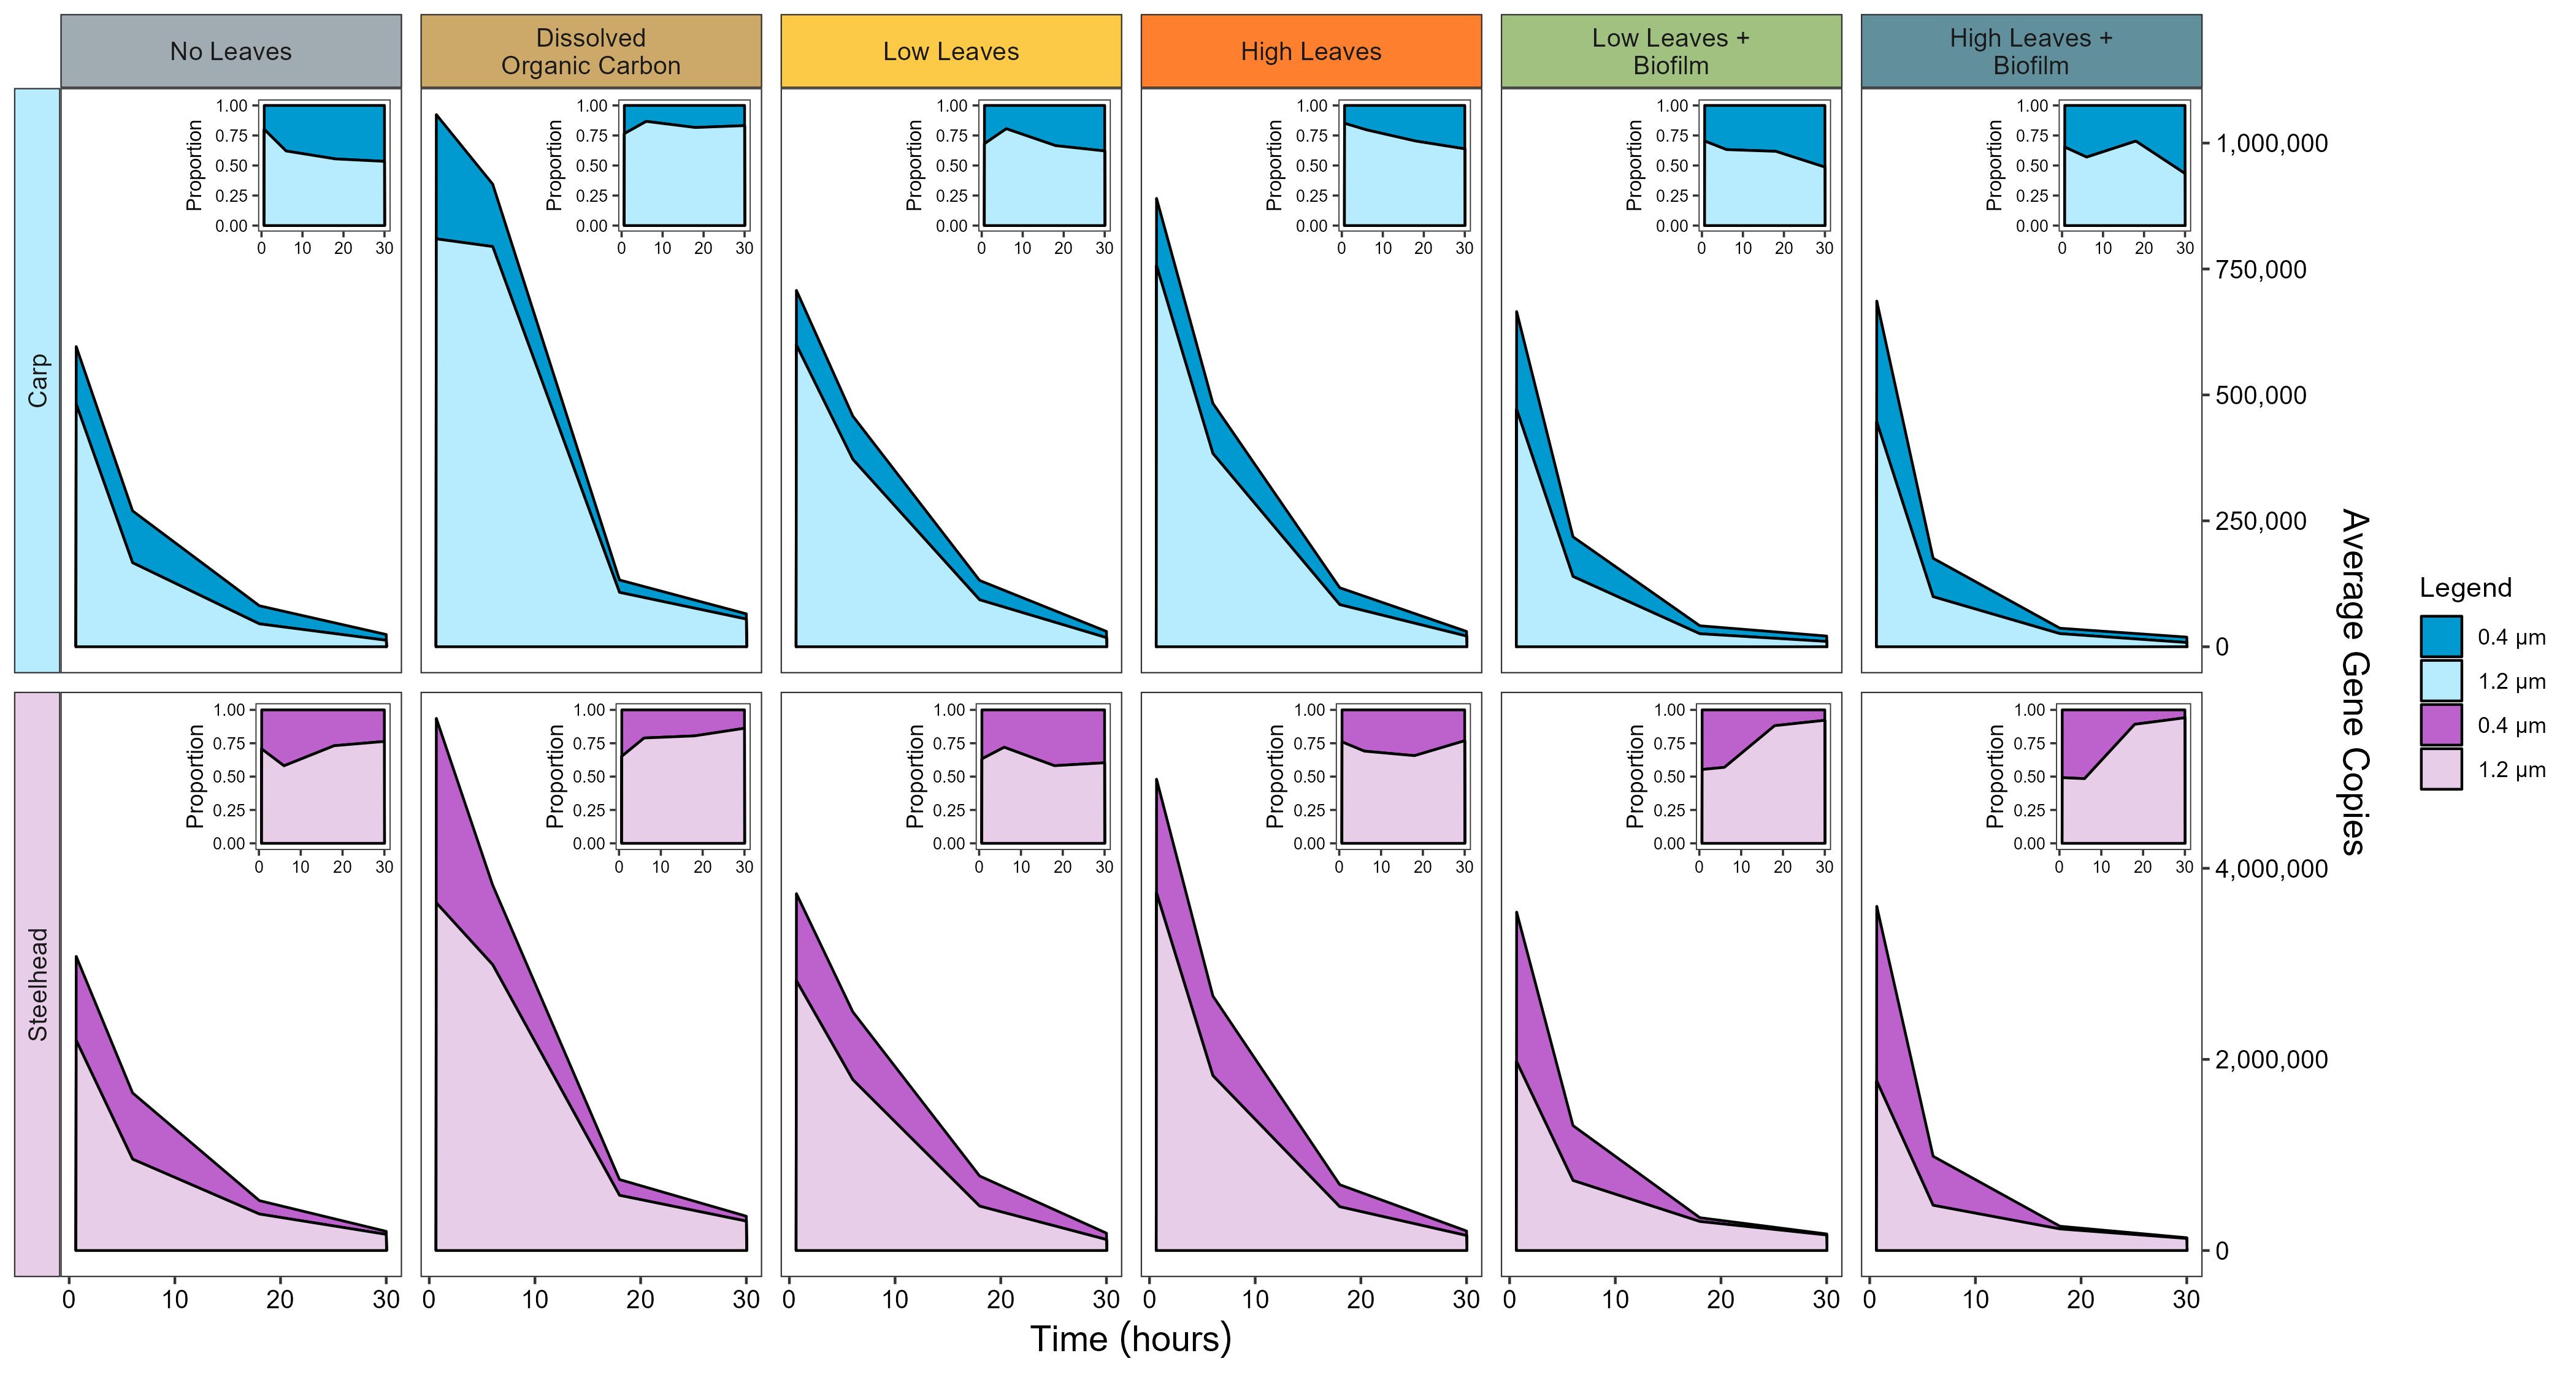
\includegraphics[width=58.33in]{Plots/Fig2}

\begin{verbatim}
## `geom_smooth()` using formula = 'y ~ x'
\end{verbatim}

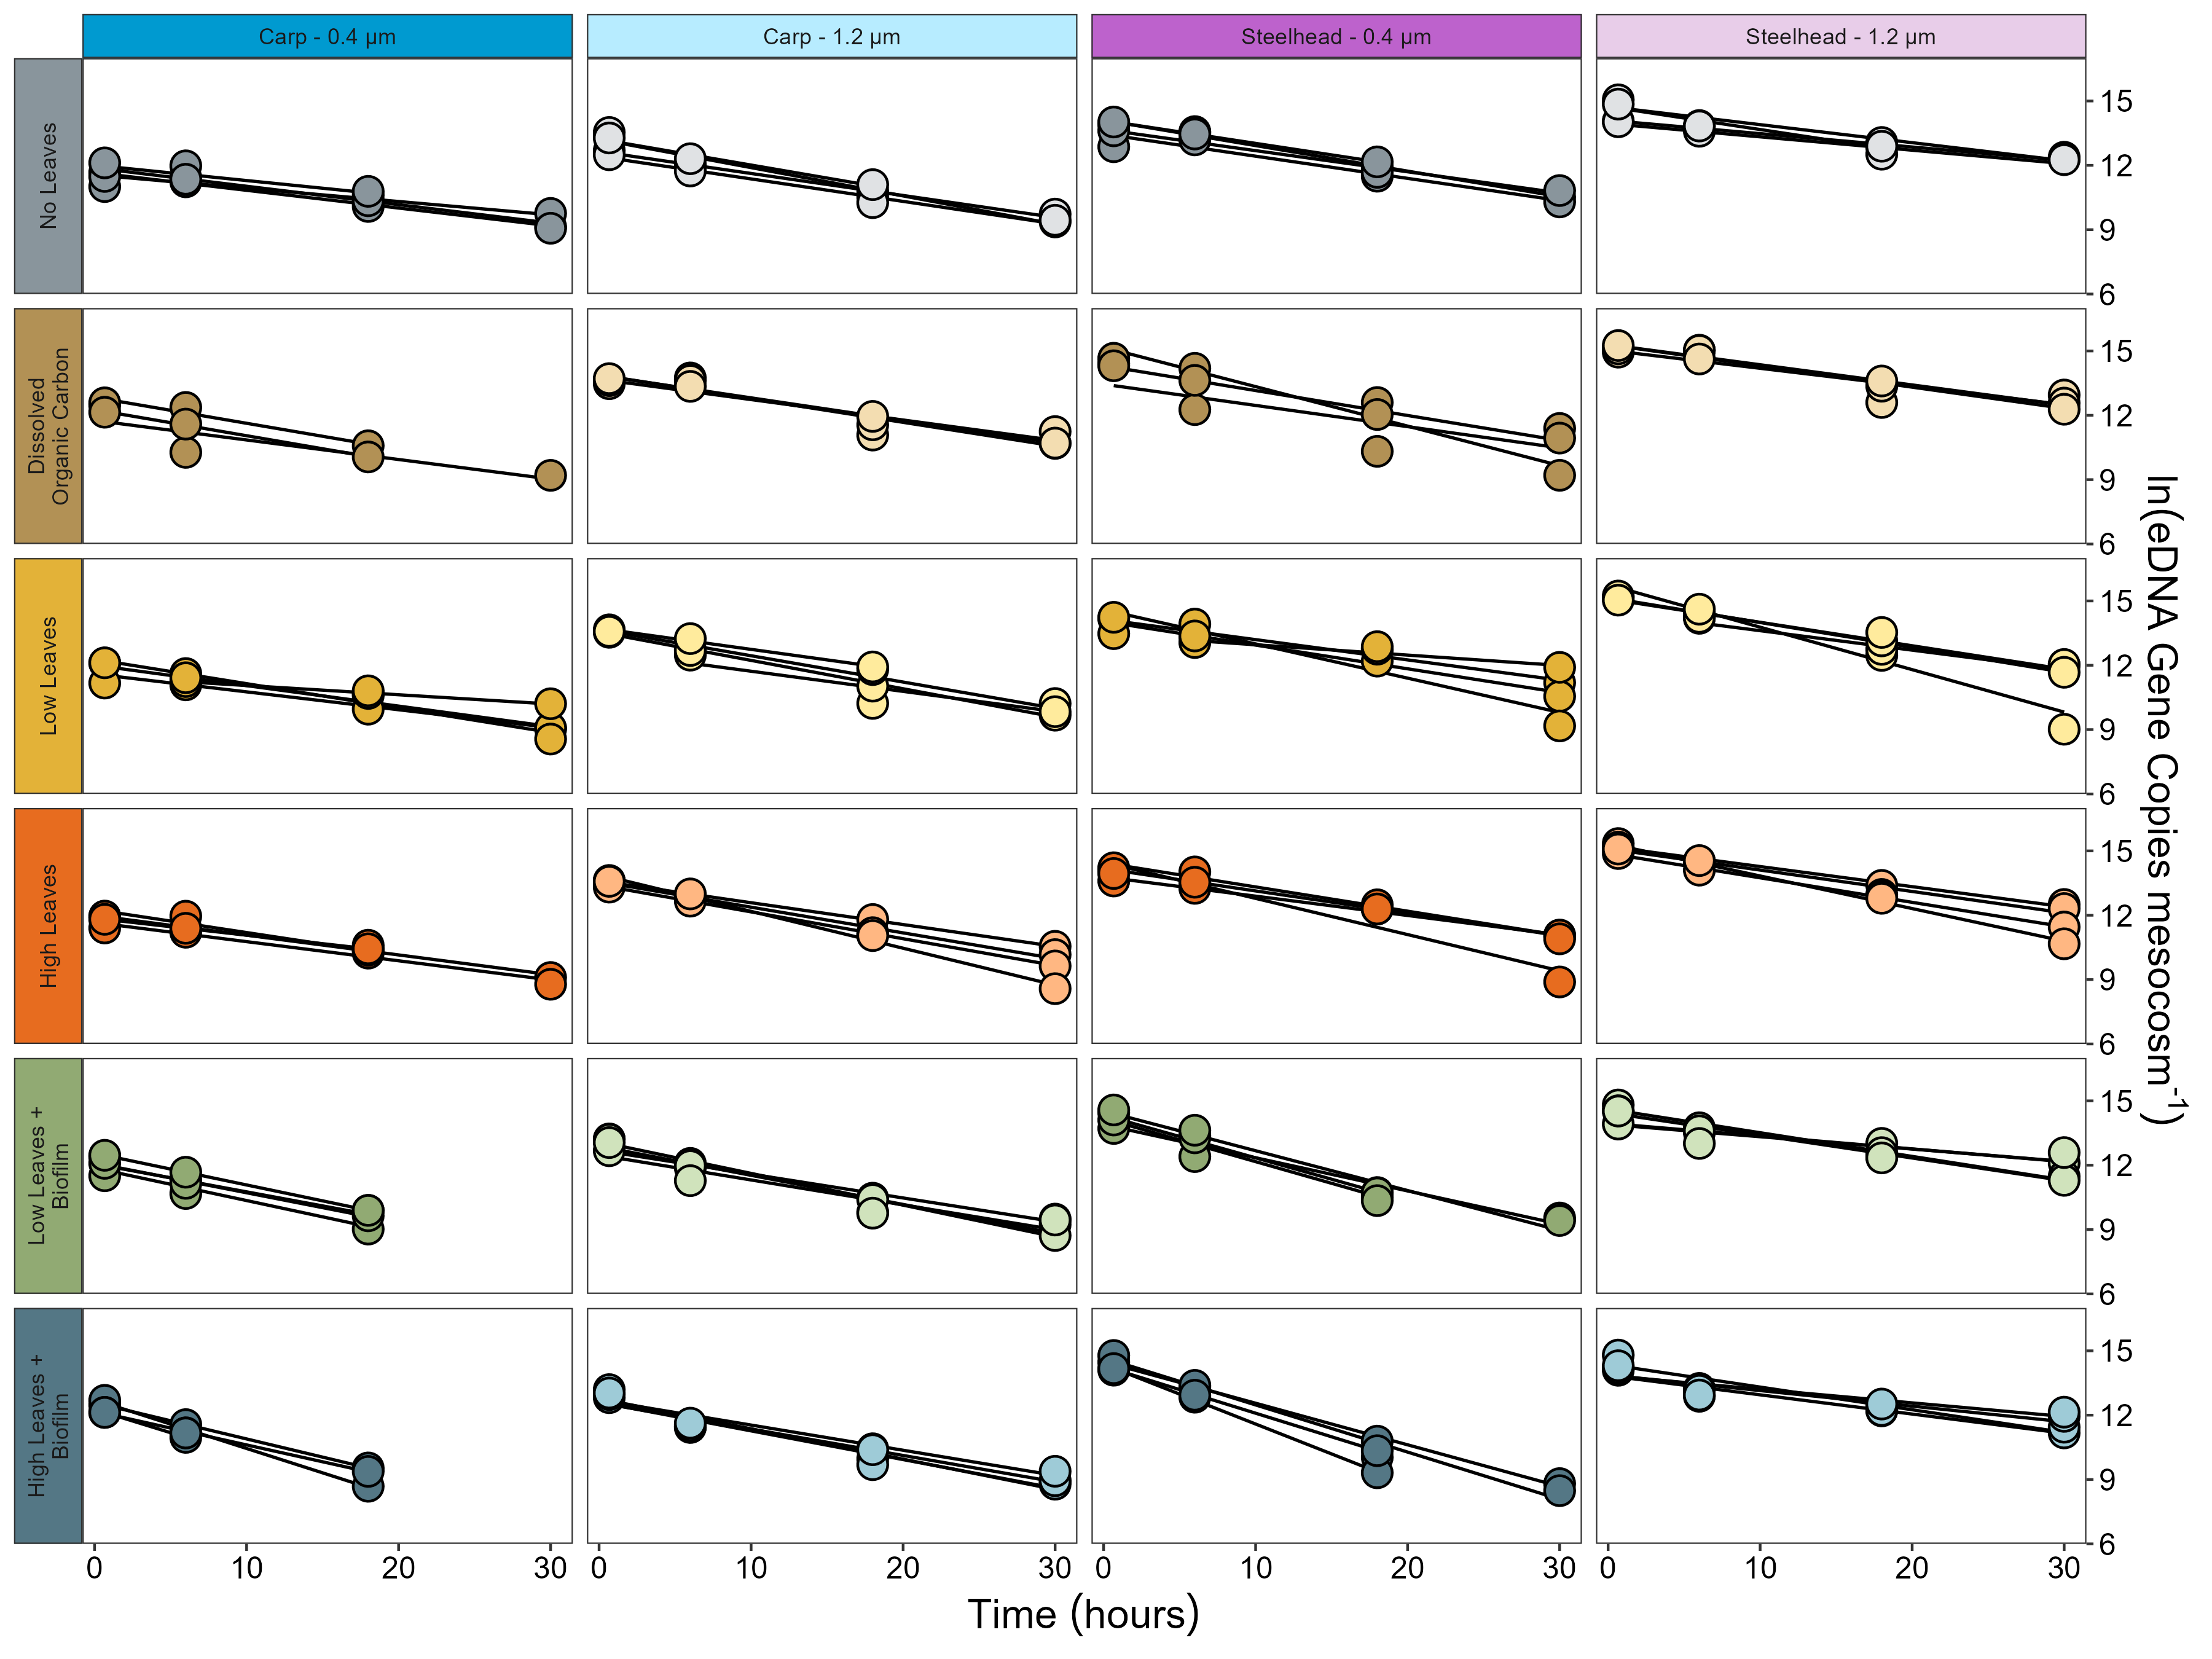
\includegraphics[width=50in]{Plots/Fig3}
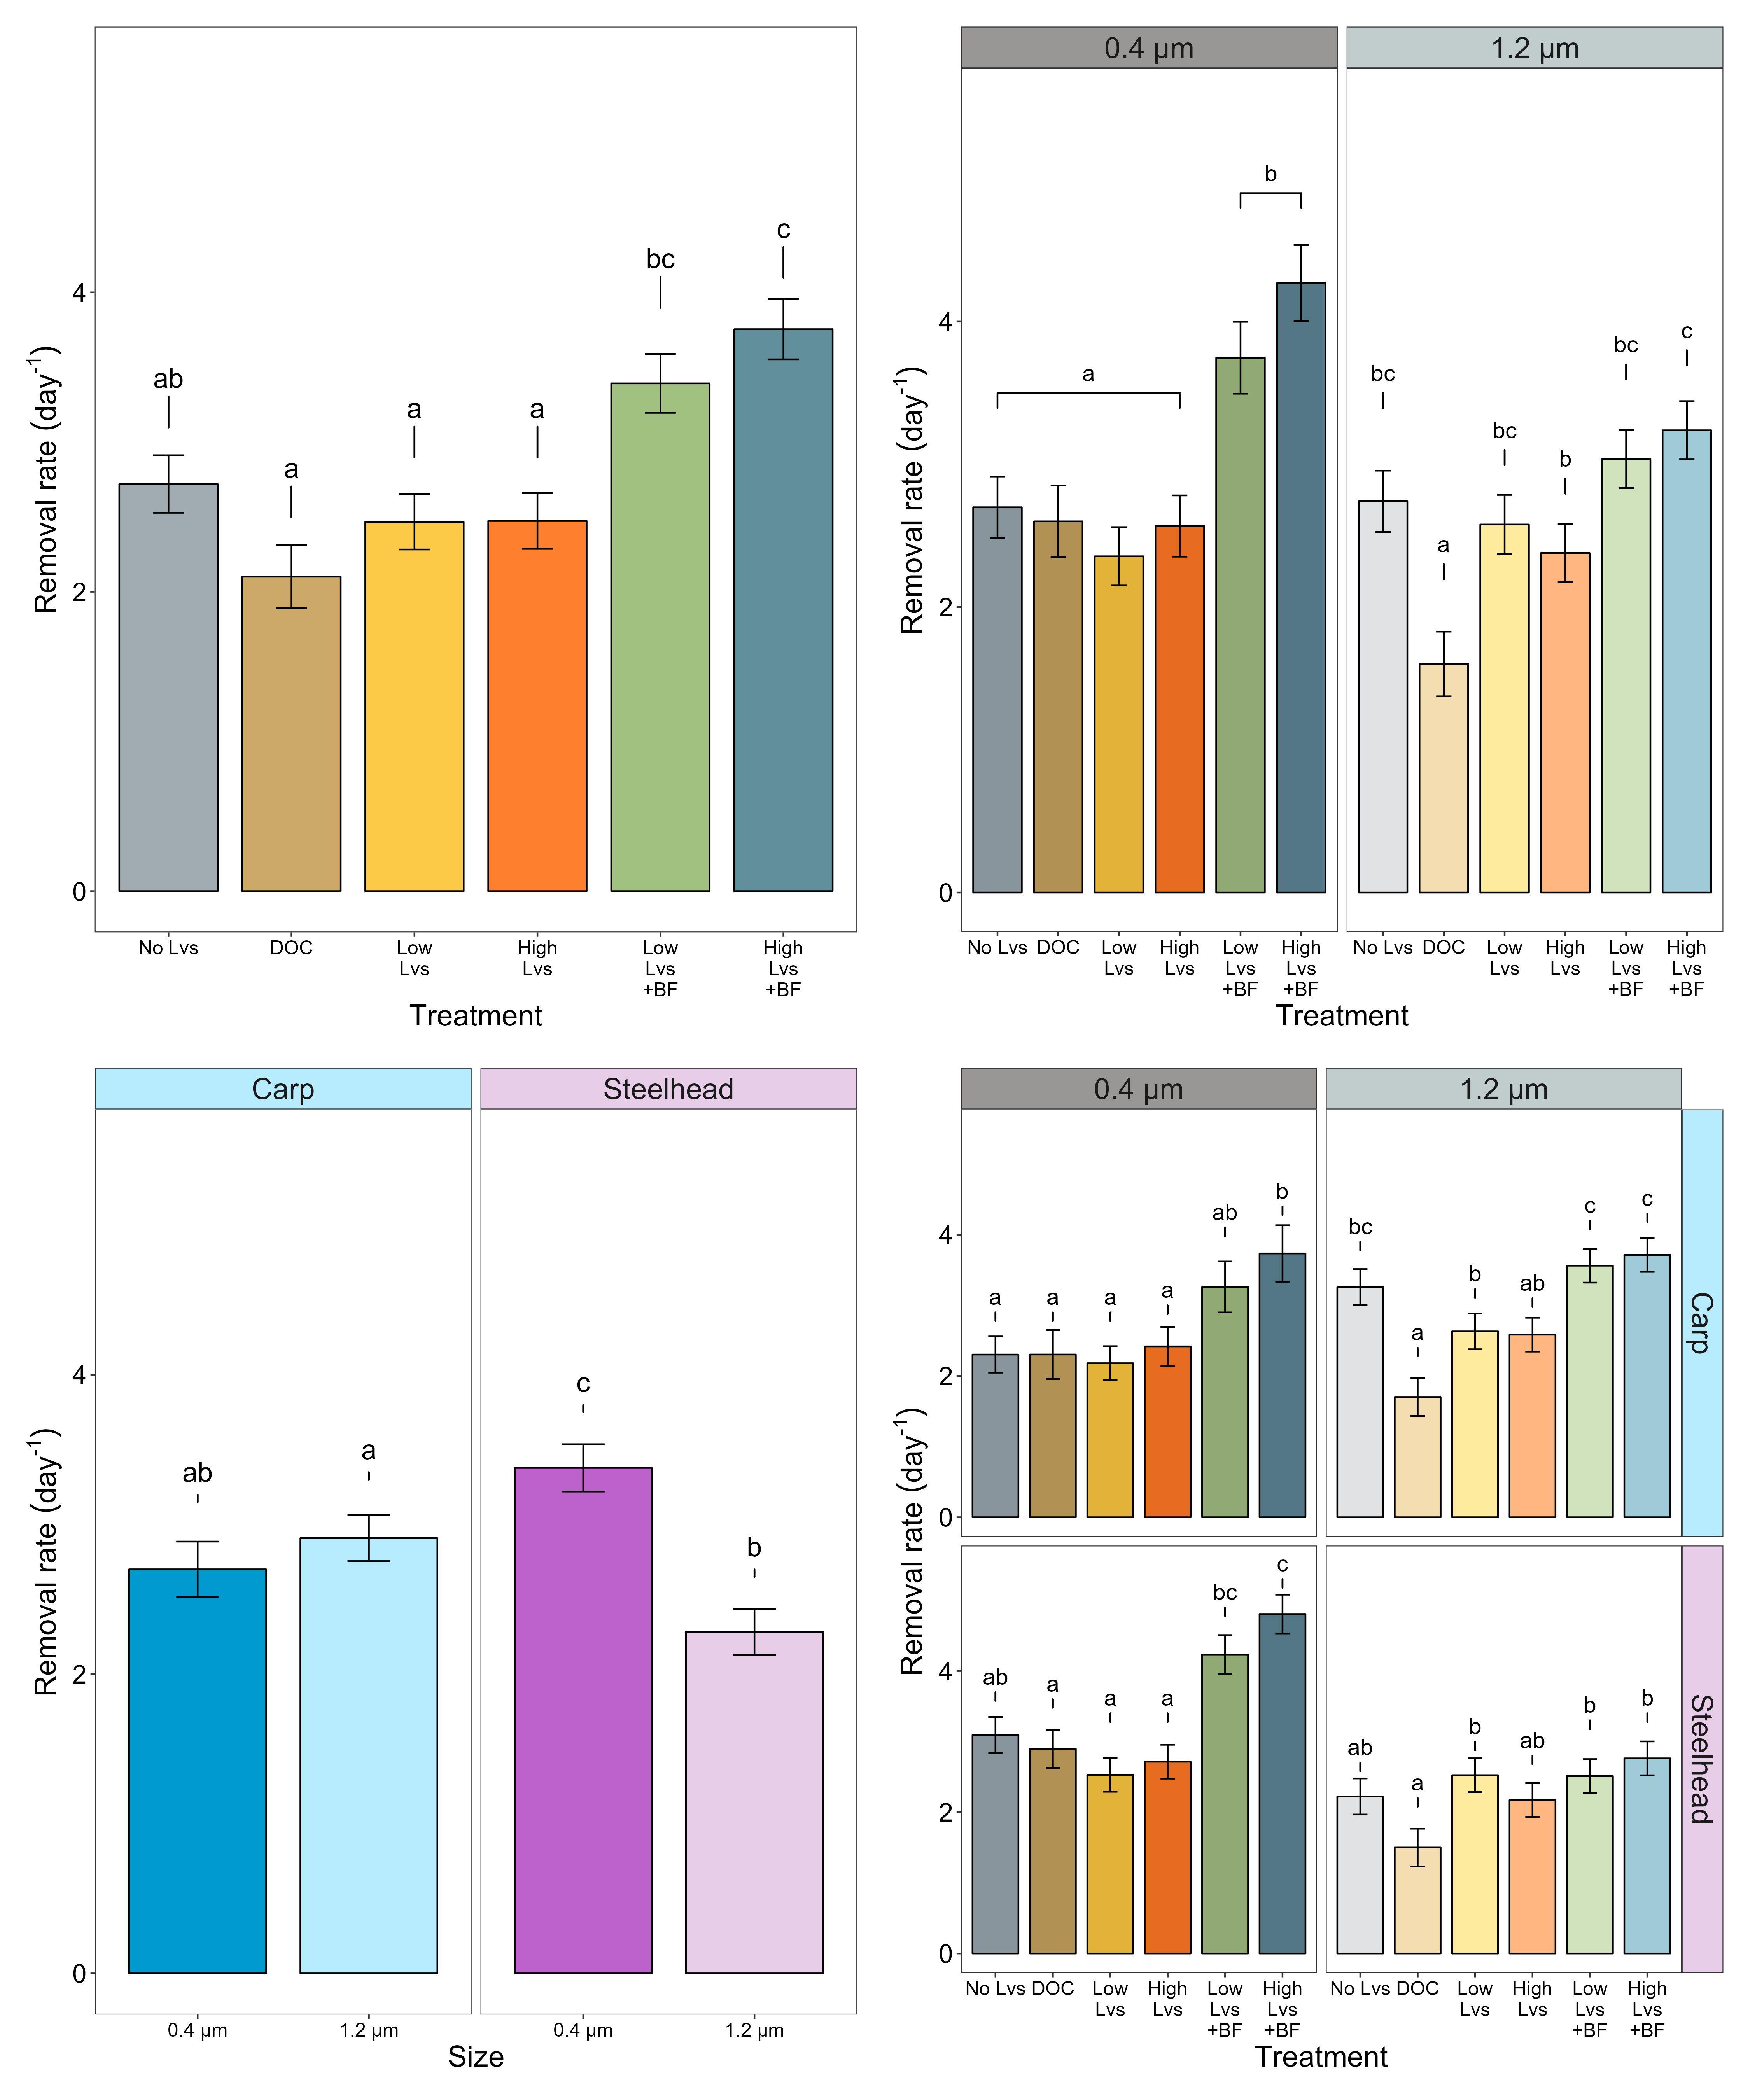
\includegraphics[width=62.5in]{Plots/Fig4}
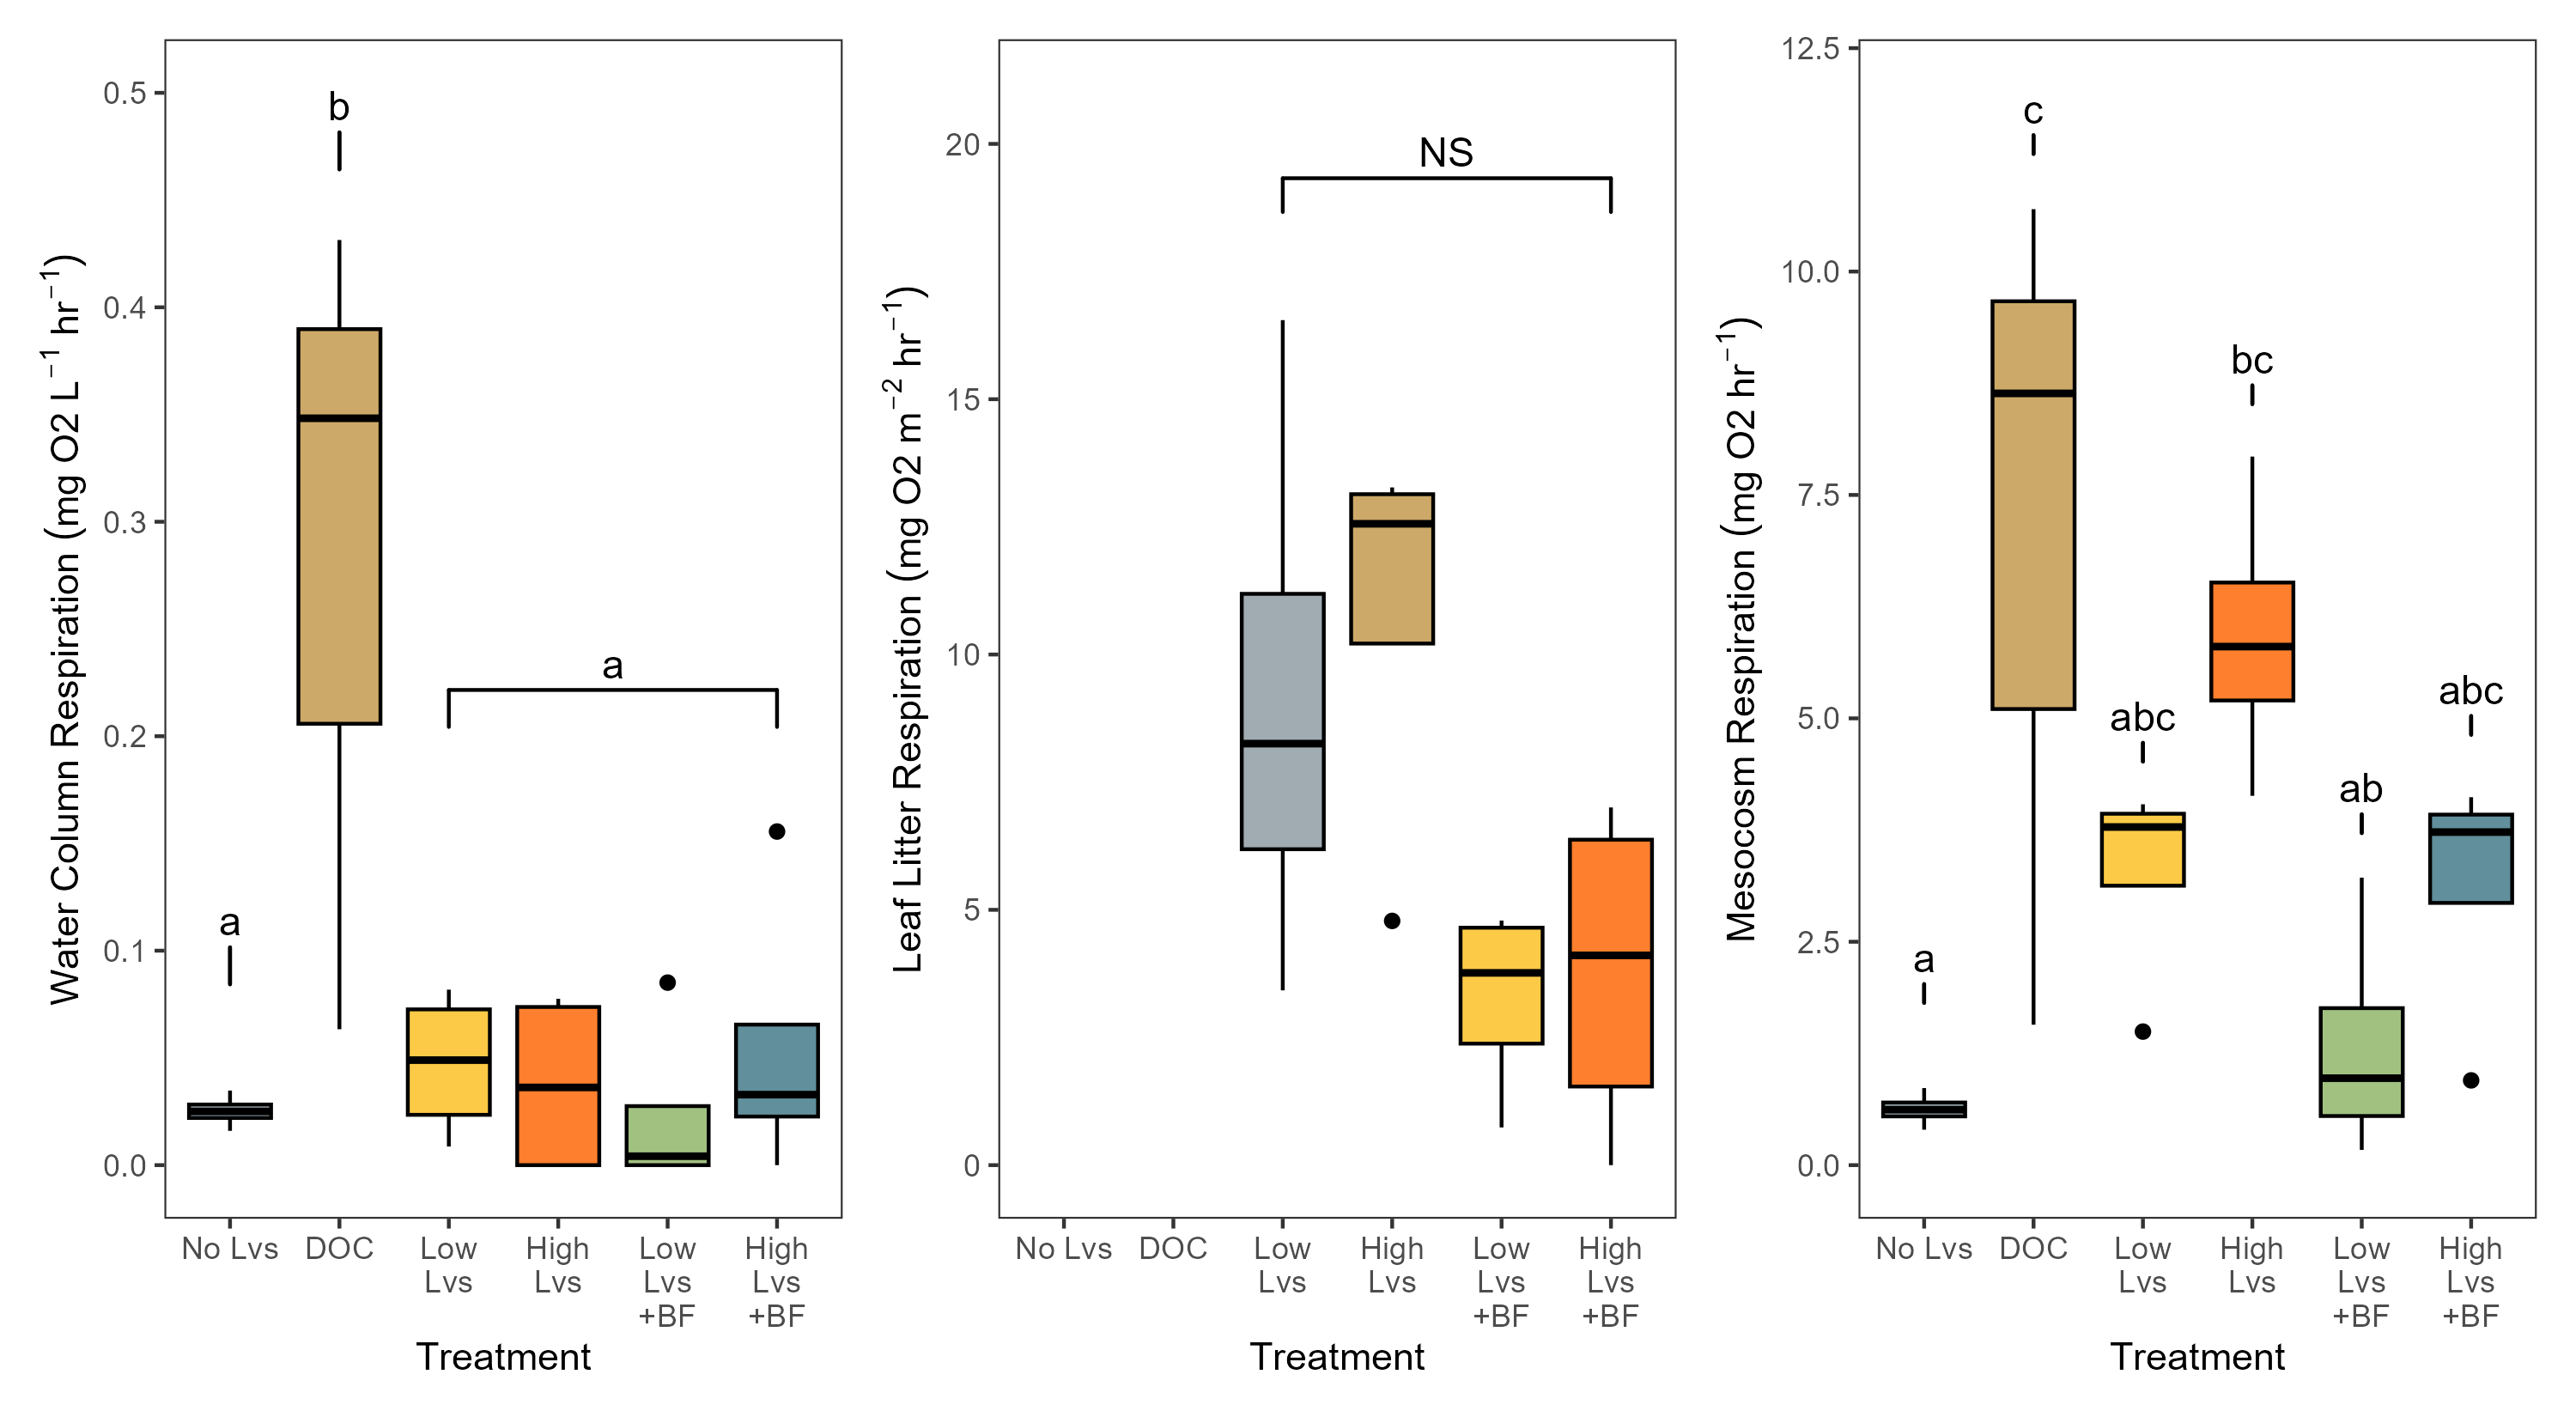
\includegraphics[width=41.67in]{Plots/Fig5}

\section{4. Supplementary Materials}\label{supplementary-materials}

Here we reproduce the materials provided in
``Supplementary\_Figures\&Tables.pdf''

\begin{Shaded}
\begin{Highlighting}[]
\CommentTok{\#Figure S0}
\NormalTok{headernames }\OtherTok{\textless{}{-}} \FunctionTok{c}\NormalTok{(}
  \StringTok{\textasciigrave{}}\AttributeTok{CARP}\StringTok{\textasciigrave{}} \OtherTok{=} \StringTok{"Carp"}\NormalTok{,}
  \StringTok{\textasciigrave{}}\AttributeTok{STHD}\StringTok{\textasciigrave{}} \OtherTok{=} \StringTok{"Steelhead"}\NormalTok{,}
  \StringTok{\textasciigrave{}}\AttributeTok{ETO}\StringTok{\textasciigrave{}} \OtherTok{=} \FunctionTok{str\_wrap}\NormalTok{(}\StringTok{"No Leaves"}\NormalTok{,}\DecValTok{15}\NormalTok{),}
  \StringTok{\textasciigrave{}}\AttributeTok{DOC}\StringTok{\textasciigrave{}} \OtherTok{=} \FunctionTok{str\_wrap}\NormalTok{(}\StringTok{"Dissolved Organic Carbon"}\NormalTok{,}\DecValTok{15}\NormalTok{),}
  \StringTok{\textasciigrave{}}\AttributeTok{NCH}\StringTok{\textasciigrave{}} \OtherTok{=} \FunctionTok{str\_wrap}\NormalTok{(}\StringTok{"High Leaves"}\NormalTok{,}\DecValTok{15}\NormalTok{),}
  \StringTok{\textasciigrave{}}\AttributeTok{NCL}\StringTok{\textasciigrave{}} \OtherTok{=} \FunctionTok{str\_wrap}\NormalTok{(}\StringTok{"Low Leaves"}\NormalTok{,}\DecValTok{15}\NormalTok{),}
  \StringTok{\textasciigrave{}}\AttributeTok{BFH}\StringTok{\textasciigrave{}} \OtherTok{=} \FunctionTok{str\_wrap}\NormalTok{(}\StringTok{"High Leaves + Biofilm"}\NormalTok{,}\DecValTok{15}\NormalTok{),}
  \StringTok{\textasciigrave{}}\AttributeTok{BFL}\StringTok{\textasciigrave{}} \OtherTok{=} \FunctionTok{str\_wrap}\NormalTok{(}\StringTok{"Low Leaves + Biofilm"}\NormalTok{,}\DecValTok{15}\NormalTok{)}
\NormalTok{)}

\NormalTok{Prop\_plot }\OtherTok{\textless{}{-}} \FunctionTok{ggplot}\NormalTok{(Mesos.prop }\SpecialCharTok{\%\textgreater{}\%} \FunctionTok{subset}\NormalTok{(prop}\SpecialCharTok{!=}\DecValTok{1} \SpecialCharTok{\&}\NormalTok{ prop}\SpecialCharTok{!=}\DecValTok{0}\NormalTok{), }\FunctionTok{aes}\NormalTok{(Time.hr, prop, }\AttributeTok{fill=}\FunctionTok{interaction}\NormalTok{(Size, Target, }\AttributeTok{sep =} \StringTok{":"}\NormalTok{ ))) }\SpecialCharTok{+}
  \FunctionTok{geom\_smooth}\NormalTok{(}\FunctionTok{aes}\NormalTok{(}\AttributeTok{group=}\NormalTok{Size, }\AttributeTok{color=}\FunctionTok{interaction}\NormalTok{(Size, Target, }\AttributeTok{sep =} \StringTok{":"}\NormalTok{ )), }
                \AttributeTok{method=}\StringTok{\textquotesingle{}lm\textquotesingle{}}\NormalTok{, }\AttributeTok{linetype=}\StringTok{"solid"}\NormalTok{, }\AttributeTok{size=}\DecValTok{1}\NormalTok{)}\SpecialCharTok{+}
  \FunctionTok{geom\_point}\NormalTok{(}\AttributeTok{size=}\DecValTok{3}\NormalTok{, }\AttributeTok{shape=}\DecValTok{21}\NormalTok{, }\AttributeTok{color=}\StringTok{"black"}\NormalTok{, }\AttributeTok{stroke=}\FloatTok{0.25}\NormalTok{)}\SpecialCharTok{+}
  \FunctionTok{scale\_fill\_manual}\NormalTok{(}\AttributeTok{values=}\FunctionTok{c}\NormalTok{(}\StringTok{"\#009AD0"}\NormalTok{,}\StringTok{"\#B7ECFF"}\NormalTok{,}\StringTok{"\#BD62CC"}\NormalTok{,}\StringTok{"\#E8CDE9"}\NormalTok{), }
                    \AttributeTok{labels=}\FunctionTok{c}\NormalTok{(}\StringTok{\textquotesingle{}0.4 μm\textquotesingle{}}\NormalTok{, }\StringTok{\textquotesingle{}1.2 μm\textquotesingle{}}\NormalTok{, }\StringTok{\textquotesingle{}0.4 μm\textquotesingle{}}\NormalTok{, }\StringTok{\textquotesingle{}1.2 μm\textquotesingle{}}\NormalTok{))}\SpecialCharTok{+}
  \FunctionTok{scale\_color\_manual}\NormalTok{(}\AttributeTok{values=}\FunctionTok{c}\NormalTok{(}\StringTok{"\#009AD0"}\NormalTok{,}\StringTok{"\#B7ECFF"}\NormalTok{,}\StringTok{"\#BD62CC"}\NormalTok{,}\StringTok{"\#E8CDE9"}\NormalTok{), }
                    \AttributeTok{labels=}\FunctionTok{c}\NormalTok{(}\StringTok{\textquotesingle{}0.4 μm\textquotesingle{}}\NormalTok{, }\StringTok{\textquotesingle{}1.2 μm\textquotesingle{}}\NormalTok{, }\StringTok{\textquotesingle{}0.4 μm\textquotesingle{}}\NormalTok{, }\StringTok{\textquotesingle{}1.2 μm\textquotesingle{}}\NormalTok{))}\SpecialCharTok{+}
  \FunctionTok{theme\_bw}\NormalTok{()}\SpecialCharTok{+}\FunctionTok{theme}\NormalTok{(}\AttributeTok{panel.grid.major =} \FunctionTok{element\_blank}\NormalTok{(), }\AttributeTok{panel.grid.minor =} \FunctionTok{element\_blank}\NormalTok{())}\SpecialCharTok{+}
  \FunctionTok{ylab}\NormalTok{(}\FunctionTok{expression}\NormalTok{(Proportion}\SpecialCharTok{\textasciitilde{}}\NormalTok{of}\SpecialCharTok{\textasciitilde{}}\NormalTok{eDNA}\SpecialCharTok{\textasciitilde{}}\NormalTok{Gene}\SpecialCharTok{\textasciitilde{}}\NormalTok{Copies}\SpecialCharTok{\textasciitilde{}}\NormalTok{Mesocosm}\SpecialCharTok{\^{}}\StringTok{"{-}1"}\NormalTok{))}\SpecialCharTok{+}
  \FunctionTok{xlab}\NormalTok{(}\FunctionTok{expression}\NormalTok{(Time}\SpecialCharTok{\textasciitilde{}}\NormalTok{(hr)))}\SpecialCharTok{+}
  \FunctionTok{theme}\NormalTok{(}\AttributeTok{axis.text.y=}\FunctionTok{element\_text}\NormalTok{(}\AttributeTok{size=}\DecValTok{11}\NormalTok{,}\AttributeTok{color=}\StringTok{"black"}\NormalTok{))}\SpecialCharTok{+}
  \FunctionTok{theme}\NormalTok{(}\AttributeTok{axis.text.x=}\FunctionTok{element\_text}\NormalTok{(}\AttributeTok{size=}\DecValTok{11}\NormalTok{,}\AttributeTok{color=}\StringTok{"black"}\NormalTok{))}\SpecialCharTok{+}
  \FunctionTok{theme}\NormalTok{(}\AttributeTok{axis.title.x=}\FunctionTok{element\_text}\NormalTok{(}\AttributeTok{size=}\DecValTok{11}\NormalTok{,}\AttributeTok{color=}\StringTok{"black"}\NormalTok{))}\SpecialCharTok{+}
  \FunctionTok{theme}\NormalTok{(}\AttributeTok{axis.title.y=}\FunctionTok{element\_text}\NormalTok{(}\AttributeTok{size=}\DecValTok{11}\NormalTok{,}\AttributeTok{color=}\StringTok{"black"}\NormalTok{))}\SpecialCharTok{+}
  \FunctionTok{theme}\NormalTok{(}\AttributeTok{legend.position=}\StringTok{"right"}\NormalTok{)}\SpecialCharTok{+}
  \FunctionTok{facet\_grid}\NormalTok{(Target}\SpecialCharTok{\textasciitilde{}}\NormalTok{Treatment, }\AttributeTok{labeller=}\FunctionTok{as\_labeller}\NormalTok{(headernames))}\SpecialCharTok{+}
  \FunctionTok{theme}\NormalTok{(}\AttributeTok{strip.text.x =} \FunctionTok{element\_text}\NormalTok{(}\AttributeTok{size=}\DecValTok{11}\NormalTok{),}
        \AttributeTok{strip.text.y =} \FunctionTok{element\_text}\NormalTok{(}\AttributeTok{size=}\DecValTok{11}\NormalTok{),}
        \AttributeTok{panel.spacing =} \FunctionTok{unit}\NormalTok{(}\FloatTok{0.7}\NormalTok{, }\StringTok{"lines"}\NormalTok{))}\SpecialCharTok{+}
  \FunctionTok{labs}\NormalTok{(}\AttributeTok{fill =} \StringTok{"Legend"}\NormalTok{)}\SpecialCharTok{+}
  \FunctionTok{labs}\NormalTok{(}\AttributeTok{color =} \StringTok{"Legend"}\NormalTok{)}
\NormalTok{Prop\_plot }\OtherTok{\textless{}{-}} \FunctionTok{facetColor}\NormalTok{(Prop\_plot, }\FunctionTok{c}\NormalTok{(p7}\FloatTok{.5}\NormalTok{,}\StringTok{"\#B7ECFF"}\NormalTok{,}\StringTok{"\#E8CDE9"}\NormalTok{))}
\end{Highlighting}
\end{Shaded}

\begin{verbatim}
## `geom_smooth()` using formula = 'y ~ x'
\end{verbatim}

\begin{Shaded}
\begin{Highlighting}[]
\FunctionTok{ggsave}\NormalTok{(}\FunctionTok{paste0}\NormalTok{(plots.dir,}\StringTok{"/FigS0.png"}\NormalTok{), Prop\_plot, }\AttributeTok{width =} \DecValTok{14}\NormalTok{, }\AttributeTok{height =}\FloatTok{7.5}\NormalTok{, }\AttributeTok{units =} \FunctionTok{c}\NormalTok{(}\StringTok{"in"}\NormalTok{))}

\NormalTok{knitr}\SpecialCharTok{::}\FunctionTok{include\_graphics}\NormalTok{(}\FunctionTok{paste0}\NormalTok{(plots.dir,}\StringTok{"/FigS0.png"}\NormalTok{))}
\end{Highlighting}
\end{Shaded}

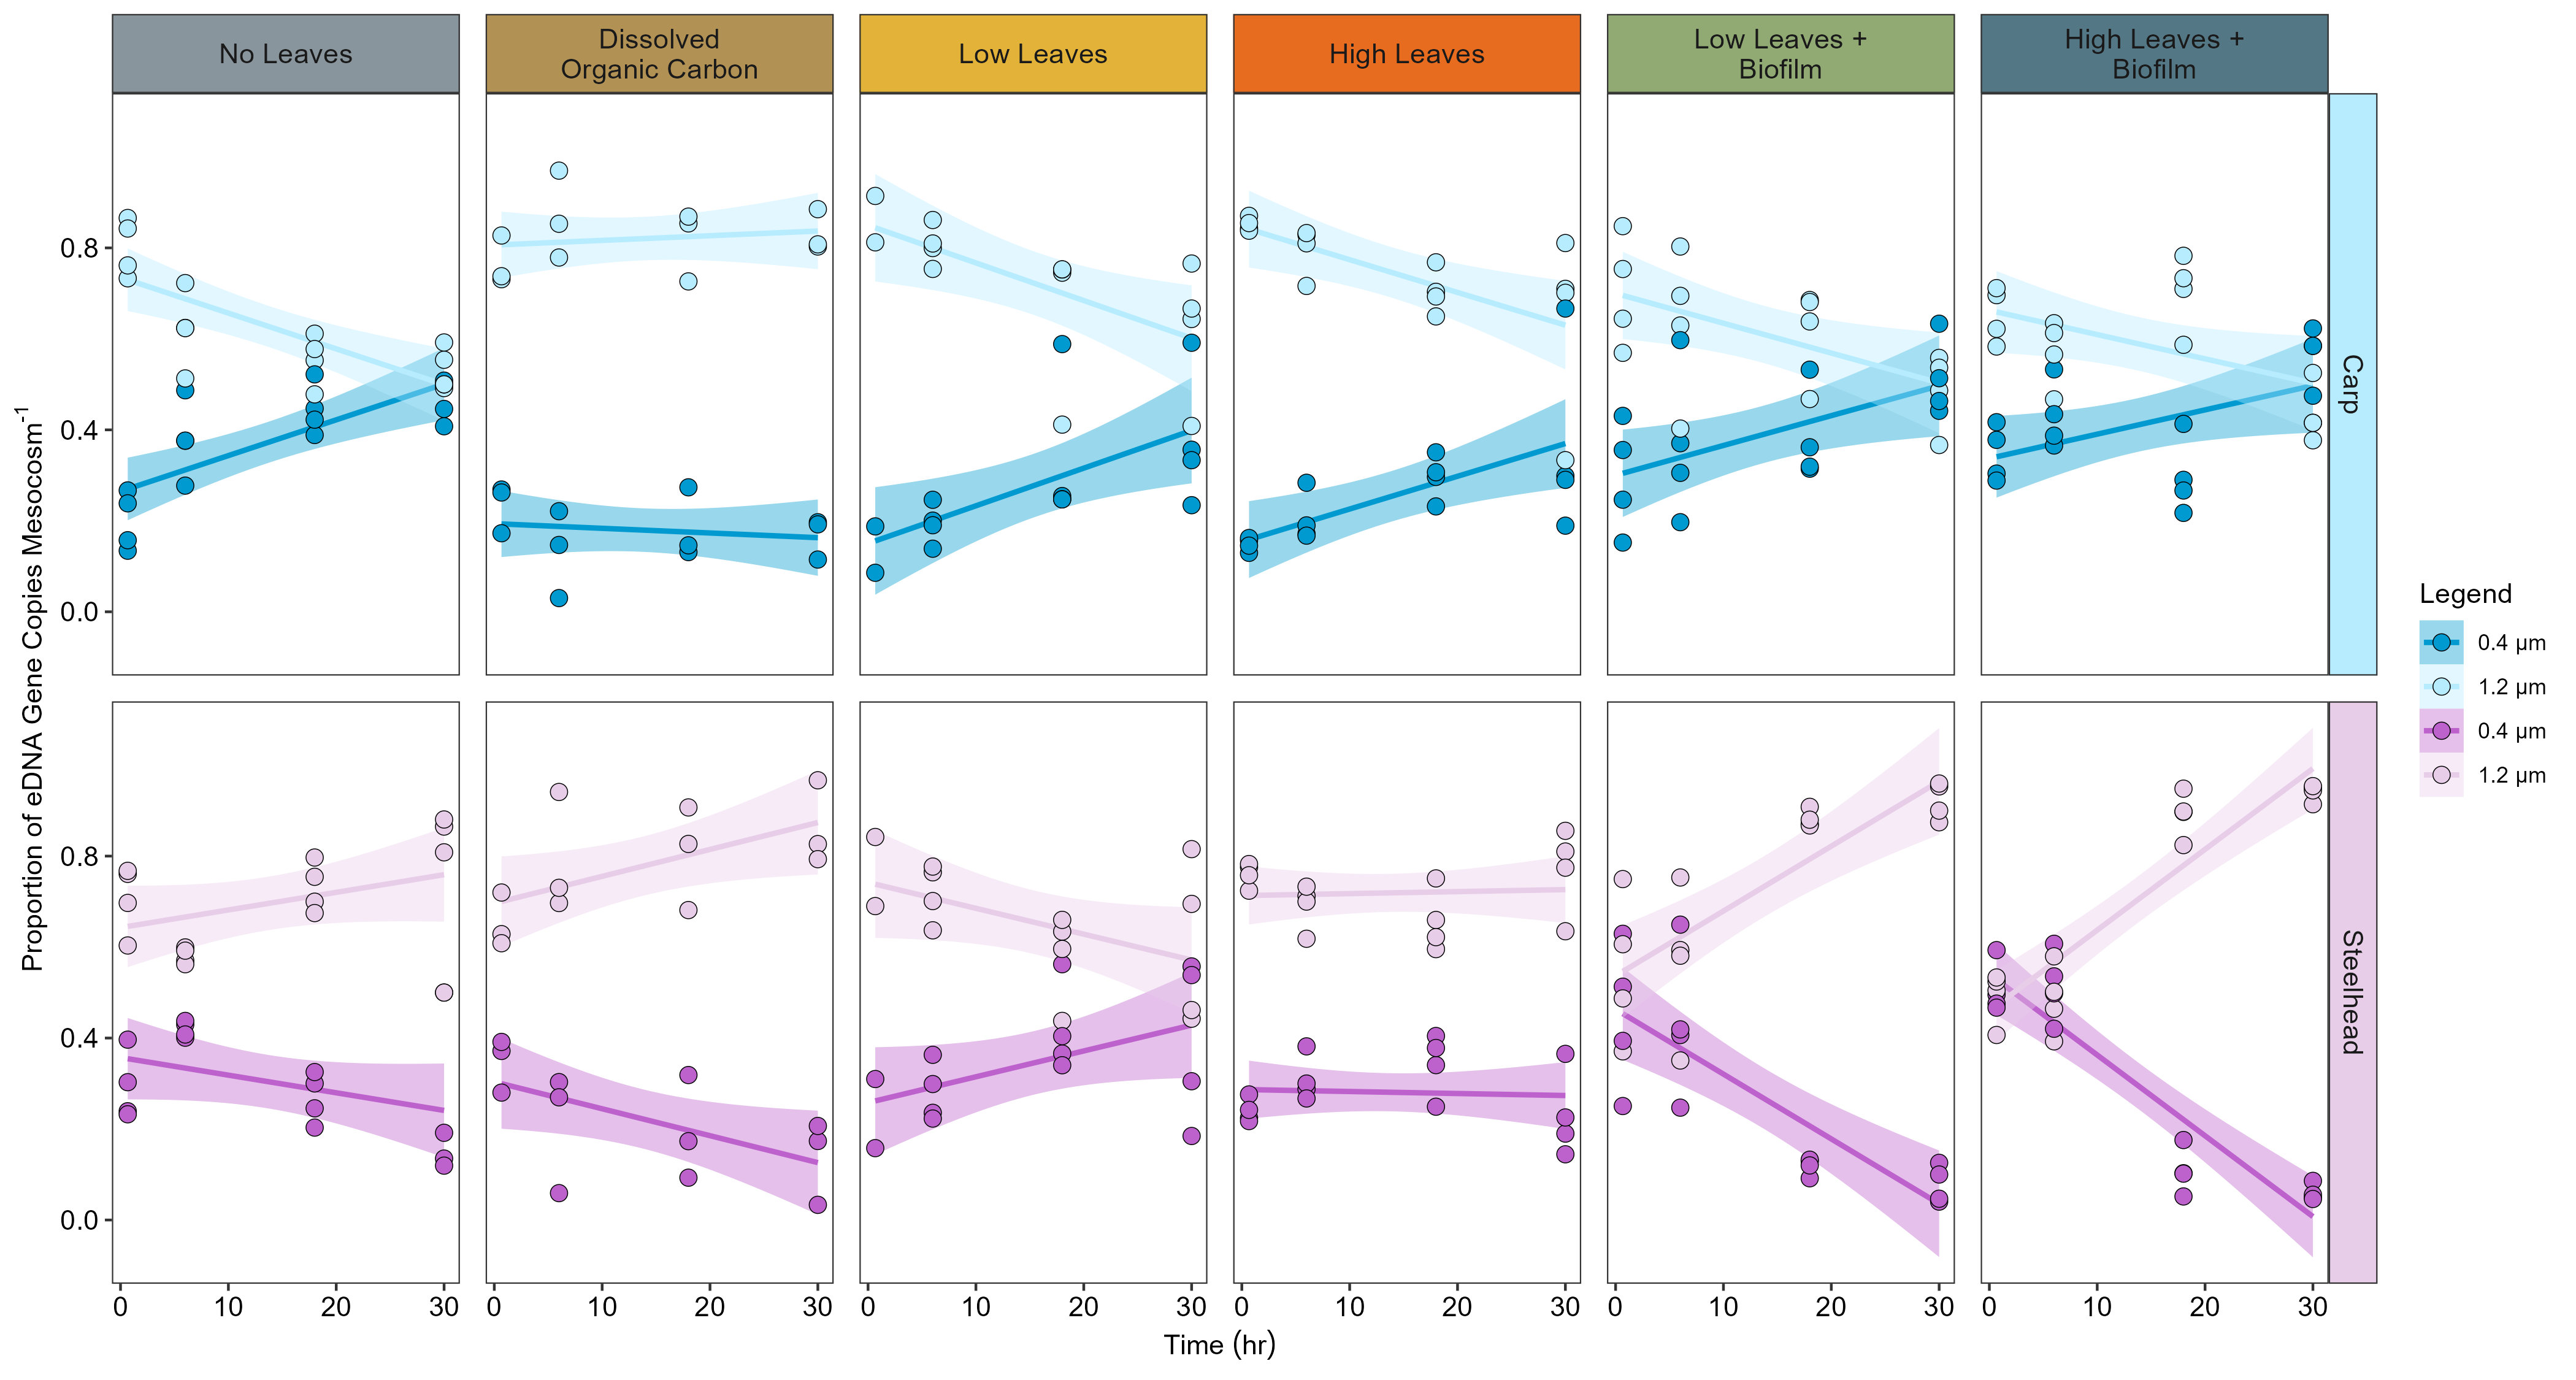
\includegraphics[width=58.33in]{Plots/FigS0}

\begin{Shaded}
\begin{Highlighting}[]
\CommentTok{\#Figure S1}
\CommentTok{\#Coerce}
\NormalTok{Rel}\SpecialCharTok{$}\NormalTok{Bucket }\OtherTok{\textless{}{-}} \FunctionTok{as.factor}\NormalTok{(Rel}\SpecialCharTok{$}\NormalTok{Bucket)}
\NormalTok{Rel}\SpecialCharTok{$}\NormalTok{Size }\OtherTok{\textless{}{-}} \FunctionTok{as.factor}\NormalTok{(Rel}\SpecialCharTok{$}\NormalTok{Size)}
\NormalTok{Rel}\SpecialCharTok{$}\NormalTok{Target }\OtherTok{\textless{}{-}} \FunctionTok{as.factor}\NormalTok{(Rel}\SpecialCharTok{$}\NormalTok{Target)}

\CommentTok{\#Average}
\NormalTok{Rel }\OtherTok{\textless{}{-}}\NormalTok{ Rel }\SpecialCharTok{\%\textgreater{}\%} \FunctionTok{group\_by}\NormalTok{(Bucket, Target, Size) }\SpecialCharTok{\%\textgreater{}\%} 
\NormalTok{  dplyr}\SpecialCharTok{::}\FunctionTok{summarise}\NormalTok{(}\AttributeTok{GC.mL =} \FunctionTok{mean}\NormalTok{(GC.mL))}
\end{Highlighting}
\end{Shaded}

\begin{verbatim}
## `summarise()` has grouped output by 'Bucket', 'Target'. You can override using
## the `.groups` argument.
\end{verbatim}

\begin{Shaded}
\begin{Highlighting}[]
\CommentTok{\#Plot}
\NormalTok{headernames }\OtherTok{\textless{}{-}} \FunctionTok{c}\NormalTok{(}
  \StringTok{\textasciigrave{}}\AttributeTok{CARP}\StringTok{\textasciigrave{}} \OtherTok{=} \StringTok{"Carp"}\NormalTok{,}
  \StringTok{\textasciigrave{}}\AttributeTok{STHD}\StringTok{\textasciigrave{}} \OtherTok{=} \StringTok{"Steelhead"}\NormalTok{,}
  \StringTok{\textasciigrave{}}\AttributeTok{BKT1}\StringTok{\textasciigrave{}} \OtherTok{=} \StringTok{"Row 1"}\NormalTok{,}
  \StringTok{\textasciigrave{}}\AttributeTok{BKT2}\StringTok{\textasciigrave{}} \OtherTok{=} \StringTok{"Row 2"}\NormalTok{,}
  \StringTok{\textasciigrave{}}\AttributeTok{BKT3}\StringTok{\textasciigrave{}} \OtherTok{=} \StringTok{"Row 3"}\NormalTok{,}
  \StringTok{\textasciigrave{}}\AttributeTok{BKT4}\StringTok{\textasciigrave{}} \OtherTok{=} \StringTok{"Row 4"}
\NormalTok{)}

\NormalTok{BKTA }\OtherTok{\textless{}{-}} \FunctionTok{ggplot}\NormalTok{(Rel, }\FunctionTok{aes}\NormalTok{(}\AttributeTok{x=}\NormalTok{Bucket, }\AttributeTok{y=}\NormalTok{GC.mL, }\AttributeTok{fill=}\FunctionTok{interaction}\NormalTok{(Size, Target, }\StringTok{":"}\NormalTok{))) }\SpecialCharTok{+} 
  \FunctionTok{geom\_bar}\NormalTok{(}\AttributeTok{stat =} \StringTok{"identity"}\NormalTok{, }\AttributeTok{position =} \StringTok{"stack"}\NormalTok{, }\AttributeTok{color=}\StringTok{"black"}\NormalTok{)}\SpecialCharTok{+}
  \FunctionTok{scale\_fill\_manual}\NormalTok{(}\AttributeTok{values=}\FunctionTok{c}\NormalTok{(}\StringTok{"\#009AD0"}\NormalTok{,}\StringTok{"\#B7ECFF"}\NormalTok{,}\StringTok{"\#BD62CC"}\NormalTok{,}\StringTok{"\#E8CDE9"}\NormalTok{), }\AttributeTok{labels =}\FunctionTok{c}\NormalTok{(}\StringTok{\textquotesingle{}0.4 μm\textquotesingle{}}\NormalTok{, }\StringTok{\textquotesingle{}1.2 μm\textquotesingle{}}\NormalTok{, }\StringTok{\textquotesingle{}0.4 μm\textquotesingle{}}\NormalTok{, }\StringTok{\textquotesingle{}1.2 μm\textquotesingle{}}\NormalTok{))}\SpecialCharTok{+}
  \FunctionTok{theme\_bw}\NormalTok{()}\SpecialCharTok{+}\FunctionTok{theme}\NormalTok{(}\AttributeTok{panel.grid.major =} \FunctionTok{element\_blank}\NormalTok{(), }\AttributeTok{panel.grid.minor =} \FunctionTok{element\_blank}\NormalTok{())}\SpecialCharTok{+}
  \FunctionTok{ylab}\NormalTok{(}\FunctionTok{expression}\NormalTok{(Gene}\SpecialCharTok{\textasciitilde{}}\NormalTok{Copies}\SpecialCharTok{\textasciitilde{}}\NormalTok{mL}\SpecialCharTok{\^{}}\StringTok{"{-}1"}\NormalTok{))}\SpecialCharTok{+}
  \FunctionTok{scale\_y\_continuous}\NormalTok{(}\AttributeTok{position =} \StringTok{"left"}\NormalTok{)}\SpecialCharTok{+}
  \FunctionTok{xlab}\NormalTok{(}\FunctionTok{expression}\NormalTok{(Bucket))}\SpecialCharTok{+}
  \FunctionTok{theme}\NormalTok{(}\AttributeTok{axis.text.y=}\FunctionTok{element\_text}\NormalTok{(}\AttributeTok{size=}\DecValTok{10}\NormalTok{,}\AttributeTok{color=}\StringTok{"black"}\NormalTok{))}\SpecialCharTok{+}
  \FunctionTok{theme}\NormalTok{(}\AttributeTok{axis.text.x=}\FunctionTok{element\_text}\NormalTok{(}\AttributeTok{size=}\DecValTok{10}\NormalTok{,}\AttributeTok{color=}\StringTok{"black"}\NormalTok{))}\SpecialCharTok{+}
  \FunctionTok{theme}\NormalTok{(}\AttributeTok{axis.title.x=}\FunctionTok{element\_text}\NormalTok{(}\AttributeTok{size=}\DecValTok{14}\NormalTok{,}\AttributeTok{color=}\StringTok{"black"}\NormalTok{))}\SpecialCharTok{+}
  \FunctionTok{theme}\NormalTok{(}\AttributeTok{axis.title.y=}\FunctionTok{element\_text}\NormalTok{(}\AttributeTok{size=}\DecValTok{14}\NormalTok{,}\AttributeTok{color=}\StringTok{"black"}\NormalTok{))}\SpecialCharTok{+}
  \FunctionTok{theme}\NormalTok{(}\AttributeTok{strip.background =}\FunctionTok{element\_rect}\NormalTok{(}\AttributeTok{fill=}\StringTok{"white"}\NormalTok{))}\SpecialCharTok{+}
  \FunctionTok{theme}\NormalTok{(}\AttributeTok{strip.text.x =} \FunctionTok{element\_text}\NormalTok{(}\AttributeTok{size=}\DecValTok{14}\NormalTok{),}
        \AttributeTok{strip.text.y =} \FunctionTok{element\_text}\NormalTok{(}\AttributeTok{size=}\DecValTok{14}\NormalTok{))}\SpecialCharTok{+}
  \FunctionTok{theme}\NormalTok{(}\AttributeTok{legend.position=}\StringTok{"none"}\NormalTok{)}\SpecialCharTok{+}
  \FunctionTok{facet\_wrap}\NormalTok{(}\SpecialCharTok{\textasciitilde{}}\NormalTok{Target, }\AttributeTok{labeller =} \FunctionTok{as\_labeller}\NormalTok{(headernames))}\SpecialCharTok{+}
  \FunctionTok{scale\_x\_discrete}\NormalTok{(}\AttributeTok{labels =}\NormalTok{ headernames)}
\NormalTok{BKTA }\OtherTok{\textless{}{-}} \FunctionTok{facetColor}\NormalTok{(BKTA, }\FunctionTok{c}\NormalTok{(}\StringTok{"\#B7ECFF"}\NormalTok{,}\StringTok{"\#E8CDE9"}\NormalTok{))}

\CommentTok{\#Now calculate proportions}
\NormalTok{Rel.Prop }\OtherTok{\textless{}{-}}\NormalTok{ Rel }\SpecialCharTok{\%\textgreater{}\%} 
  \FunctionTok{group\_by}\NormalTok{(Bucket, Target) }\SpecialCharTok{\%\textgreater{}\%} 
\NormalTok{  dplyr}\SpecialCharTok{::}\FunctionTok{summarise}\NormalTok{(}\AttributeTok{n =} \FunctionTok{sum}\NormalTok{(GC.mL)) }
\end{Highlighting}
\end{Shaded}

\begin{verbatim}
## `summarise()` has grouped output by 'Bucket'. You can override using the
## `.groups` argument.
\end{verbatim}

\begin{Shaded}
\begin{Highlighting}[]
\NormalTok{Rel.Prop }\OtherTok{\textless{}{-}} \FunctionTok{inner\_join}\NormalTok{(Rel, Rel.Prop, }\AttributeTok{by=}\FunctionTok{c}\NormalTok{(}\StringTok{"Bucket"}\NormalTok{, }\StringTok{"Target"}\NormalTok{))}
\NormalTok{Rel.Prop }\OtherTok{\textless{}{-}}\NormalTok{ Rel.Prop }\SpecialCharTok{\%\textgreater{}\%} \FunctionTok{mutate}\NormalTok{(}\AttributeTok{prop =}\NormalTok{ GC.mL }\SpecialCharTok{/}\NormalTok{ n)}

\CommentTok{\#plot}
\NormalTok{BKTB }\OtherTok{\textless{}{-}} \FunctionTok{ggplot}\NormalTok{(Rel.Prop, }\FunctionTok{aes}\NormalTok{(}\AttributeTok{x=}\NormalTok{Bucket, }\AttributeTok{y=}\NormalTok{prop, }\AttributeTok{fill=}\FunctionTok{interaction}\NormalTok{(Size, Target, }\StringTok{":"}\NormalTok{))) }\SpecialCharTok{+} 
  \FunctionTok{geom\_bar}\NormalTok{(}\AttributeTok{stat =} \StringTok{"identity"}\NormalTok{, }\AttributeTok{position =} \StringTok{"stack"}\NormalTok{, }\AttributeTok{color=}\StringTok{"black"}\NormalTok{)}\SpecialCharTok{+}
  \FunctionTok{scale\_fill\_manual}\NormalTok{(}\AttributeTok{values=}\FunctionTok{c}\NormalTok{(}\StringTok{"\#009AD0"}\NormalTok{,}\StringTok{"\#B7ECFF"}\NormalTok{,}\StringTok{"\#BD62CC"}\NormalTok{,}\StringTok{"\#E8CDE9"}\NormalTok{), }\AttributeTok{labels =}\FunctionTok{c}\NormalTok{(}\StringTok{\textquotesingle{}0.4 μm\textquotesingle{}}\NormalTok{, }\StringTok{\textquotesingle{}1.2 μm\textquotesingle{}}\NormalTok{, }\StringTok{\textquotesingle{}0.4 μm\textquotesingle{}}\NormalTok{, }\StringTok{\textquotesingle{}1.2 μm\textquotesingle{}}\NormalTok{))}\SpecialCharTok{+}
  \FunctionTok{theme\_bw}\NormalTok{()}\SpecialCharTok{+}\FunctionTok{theme}\NormalTok{(}\AttributeTok{panel.grid.major =} \FunctionTok{element\_blank}\NormalTok{(), }\AttributeTok{panel.grid.minor =} \FunctionTok{element\_blank}\NormalTok{())}\SpecialCharTok{+}
  \FunctionTok{ylab}\NormalTok{(}\FunctionTok{expression}\NormalTok{(Proportion}\SpecialCharTok{\textasciitilde{}}\NormalTok{of}\SpecialCharTok{\textasciitilde{}}\NormalTok{Gene}\SpecialCharTok{\textasciitilde{}}\NormalTok{Copies}\SpecialCharTok{\textasciitilde{}}\NormalTok{mL}\SpecialCharTok{\^{}}\StringTok{"{-}1"}\NormalTok{))}\SpecialCharTok{+}
  \FunctionTok{scale\_y\_continuous}\NormalTok{(}\AttributeTok{position =} \StringTok{"left"}\NormalTok{)}\SpecialCharTok{+}
  \FunctionTok{xlab}\NormalTok{(}\FunctionTok{expression}\NormalTok{(Bucket))}\SpecialCharTok{+}
  \FunctionTok{theme}\NormalTok{(}\AttributeTok{axis.text.y=}\FunctionTok{element\_text}\NormalTok{(}\AttributeTok{size=}\DecValTok{10}\NormalTok{,}\AttributeTok{color=}\StringTok{"black"}\NormalTok{))}\SpecialCharTok{+}
  \FunctionTok{theme}\NormalTok{(}\AttributeTok{axis.text.x=}\FunctionTok{element\_text}\NormalTok{(}\AttributeTok{size=}\DecValTok{10}\NormalTok{,}\AttributeTok{color=}\StringTok{"black"}\NormalTok{))}\SpecialCharTok{+}
  \FunctionTok{theme}\NormalTok{(}\AttributeTok{axis.title.x=}\FunctionTok{element\_text}\NormalTok{(}\AttributeTok{size=}\DecValTok{14}\NormalTok{,}\AttributeTok{color=}\StringTok{"black"}\NormalTok{))}\SpecialCharTok{+}
  \FunctionTok{theme}\NormalTok{(}\AttributeTok{axis.title.y=}\FunctionTok{element\_text}\NormalTok{(}\AttributeTok{size=}\DecValTok{14}\NormalTok{,}\AttributeTok{color=}\StringTok{"black"}\NormalTok{))}\SpecialCharTok{+}
  \FunctionTok{theme}\NormalTok{(}\AttributeTok{strip.background =}\FunctionTok{element\_rect}\NormalTok{(}\AttributeTok{fill=}\StringTok{"white"}\NormalTok{))}\SpecialCharTok{+}
  \FunctionTok{theme}\NormalTok{(}\AttributeTok{strip.text.x =} \FunctionTok{element\_text}\NormalTok{(}\AttributeTok{size=}\DecValTok{14}\NormalTok{),}
        \AttributeTok{strip.text.y =} \FunctionTok{element\_text}\NormalTok{(}\AttributeTok{size=}\DecValTok{14}\NormalTok{))}\SpecialCharTok{+}
  \FunctionTok{facet\_wrap}\NormalTok{(}\SpecialCharTok{\textasciitilde{}}\NormalTok{Target, }\AttributeTok{labeller =} \FunctionTok{as\_labeller}\NormalTok{(headernames))}\SpecialCharTok{+}
  \FunctionTok{labs}\NormalTok{(}\AttributeTok{fill =} \StringTok{"Legend"}\NormalTok{)}\SpecialCharTok{+}
  \FunctionTok{scale\_x\_discrete}\NormalTok{(}\AttributeTok{labels =}\NormalTok{ headernames)}
\NormalTok{BKTB }\OtherTok{\textless{}{-}} \FunctionTok{facetColor}\NormalTok{(BKTB, }\FunctionTok{c}\NormalTok{(}\StringTok{"\#B7ECFF"}\NormalTok{,}\StringTok{"\#E8CDE9"}\NormalTok{))}

\NormalTok{BKTplot }\OtherTok{\textless{}{-}} \FunctionTok{wrap\_elements}\NormalTok{(BKTA) }\SpecialCharTok{+} \FunctionTok{wrap\_elements}\NormalTok{(BKTB)}

\FunctionTok{ggsave}\NormalTok{(}\FunctionTok{paste0}\NormalTok{(plots.dir,}\StringTok{"/FigS1.png"}\NormalTok{), BKTplot, }\AttributeTok{width =} \DecValTok{12}\NormalTok{, }\AttributeTok{height =} \DecValTok{8}\NormalTok{, }\AttributeTok{units =} \FunctionTok{c}\NormalTok{(}\StringTok{"in"}\NormalTok{))}

\NormalTok{knitr}\SpecialCharTok{::}\FunctionTok{include\_graphics}\NormalTok{(}\FunctionTok{paste0}\NormalTok{(plots.dir,}\StringTok{"/FigS1.png"}\NormalTok{))}
\end{Highlighting}
\end{Shaded}

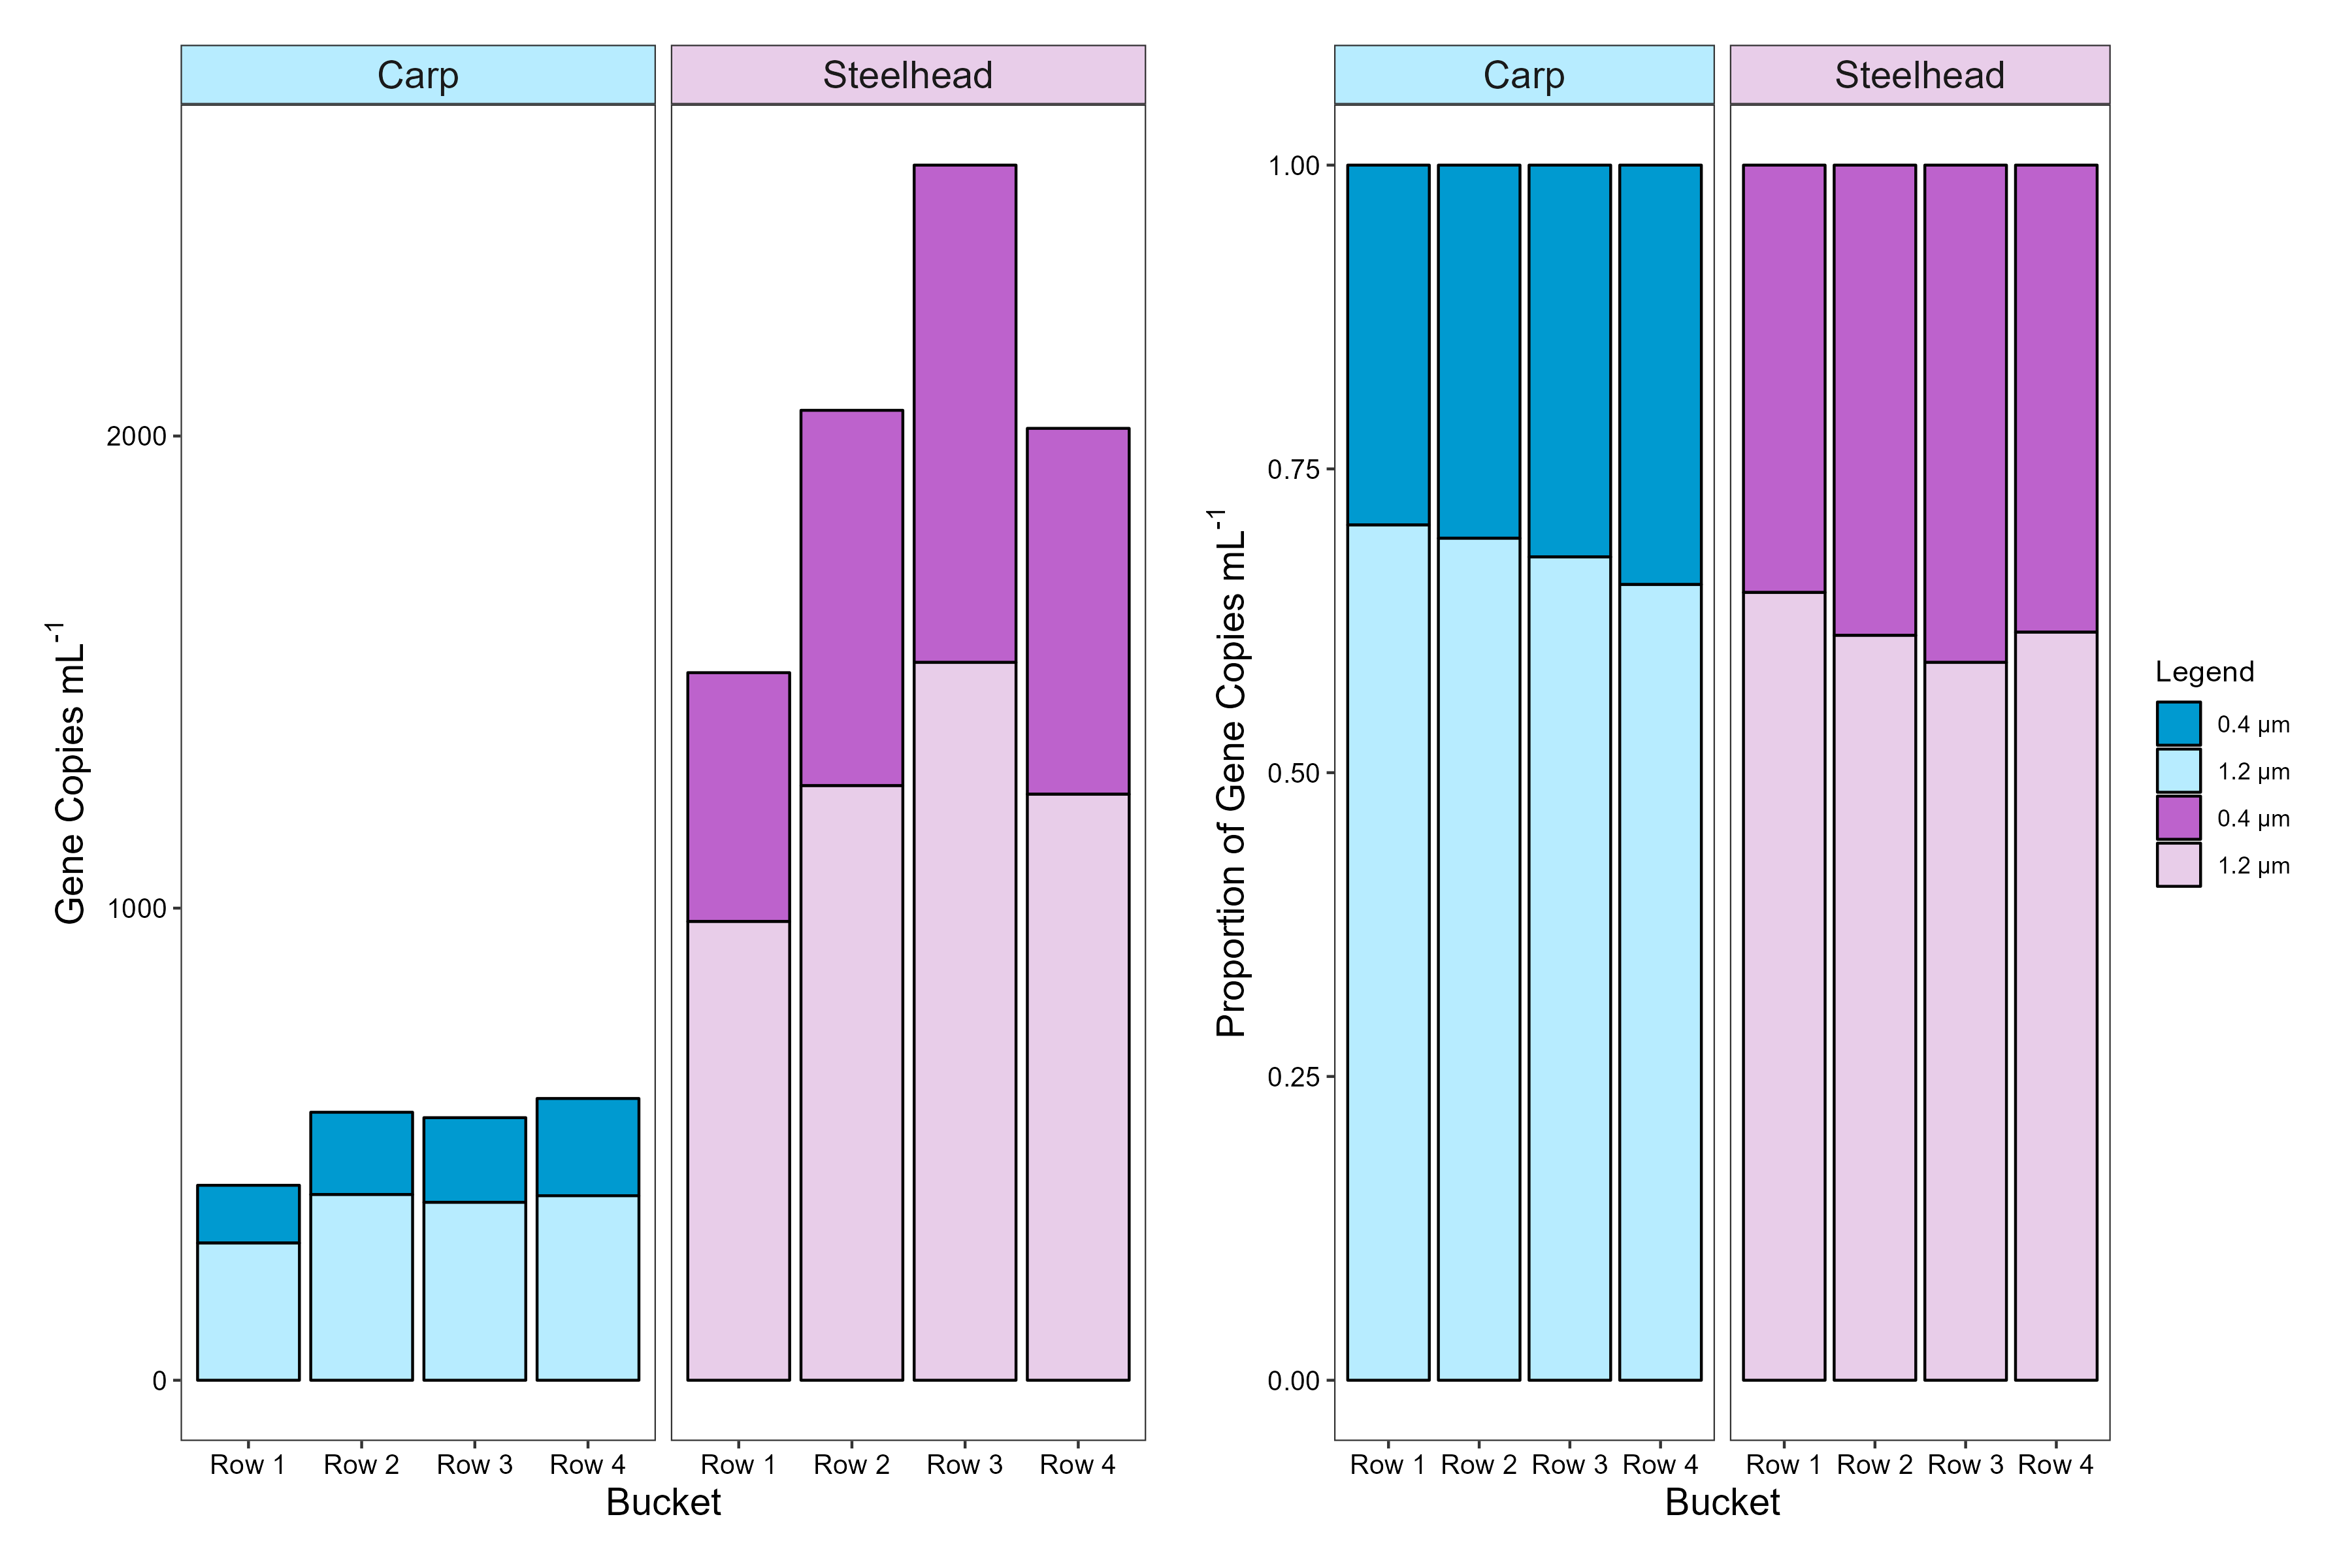
\includegraphics[width=50in]{Plots/FigS1}

\begin{Shaded}
\begin{Highlighting}[]
\CommentTok{\# Figure S2}
\FunctionTok{resid\_panel}\NormalTok{(mixed.mod, }\AttributeTok{plots=}\StringTok{"all"}\NormalTok{)}
\end{Highlighting}
\end{Shaded}

\includegraphics{Script_files/figure-latex/Supplementary-3.pdf}

\begin{Shaded}
\begin{Highlighting}[]
\FunctionTok{ggsave}\NormalTok{(}\FunctionTok{paste0}\NormalTok{(plots.dir,}\StringTok{"/FigS2.png"}\NormalTok{), }\FunctionTok{resid\_panel}\NormalTok{(mixed.mod, }\AttributeTok{plots=}\StringTok{"all"}\NormalTok{), }\AttributeTok{width =} \DecValTok{8}\NormalTok{, }\AttributeTok{height =}\DecValTok{6}\NormalTok{, }\AttributeTok{units =} \FunctionTok{c}\NormalTok{(}\StringTok{"in"}\NormalTok{))}

\CommentTok{\# Figure S3 + S4}

\CommentTok{\# Plot}
\NormalTok{headernames }\OtherTok{\textless{}{-}} \FunctionTok{c}\NormalTok{(}
  \StringTok{\textasciigrave{}}\AttributeTok{CARP}\StringTok{\textasciigrave{}} \OtherTok{=} \StringTok{"Carp"}\NormalTok{,}
  \StringTok{\textasciigrave{}}\AttributeTok{STHD}\StringTok{\textasciigrave{}} \OtherTok{=} \StringTok{"Steelhead"}\NormalTok{,}
  \StringTok{\textasciigrave{}}\AttributeTok{ETO}\StringTok{\textasciigrave{}} \OtherTok{=} \FunctionTok{str\_wrap}\NormalTok{(}\StringTok{"No Leaves"}\NormalTok{,}\DecValTok{15}\NormalTok{),}
  \StringTok{\textasciigrave{}}\AttributeTok{DOC}\StringTok{\textasciigrave{}} \OtherTok{=} \FunctionTok{str\_wrap}\NormalTok{(}\StringTok{"Dissolved Organic Carbon"}\NormalTok{,}\DecValTok{15}\NormalTok{),}
  \StringTok{\textasciigrave{}}\AttributeTok{NCH}\StringTok{\textasciigrave{}} \OtherTok{=} \FunctionTok{str\_wrap}\NormalTok{(}\StringTok{"High Leaves"}\NormalTok{,}\DecValTok{15}\NormalTok{),}
  \StringTok{\textasciigrave{}}\AttributeTok{NCL}\StringTok{\textasciigrave{}} \OtherTok{=} \FunctionTok{str\_wrap}\NormalTok{(}\StringTok{"Low Leaves"}\NormalTok{,}\DecValTok{15}\NormalTok{),}
  \StringTok{\textasciigrave{}}\AttributeTok{BFH}\StringTok{\textasciigrave{}} \OtherTok{=} \FunctionTok{str\_wrap}\NormalTok{(}\StringTok{"High Leaves + Biofilm"}\NormalTok{,}\DecValTok{15}\NormalTok{),}
  \StringTok{\textasciigrave{}}\AttributeTok{BFL}\StringTok{\textasciigrave{}} \OtherTok{=} \FunctionTok{str\_wrap}\NormalTok{(}\StringTok{"Low Leaves + Biofilm"}\NormalTok{,}\DecValTok{15}\NormalTok{),}
  \StringTok{\textasciigrave{}}\AttributeTok{1}\StringTok{\textasciigrave{}} \OtherTok{=} \StringTok{"Mesocosm 1"}\NormalTok{,}
  \StringTok{\textasciigrave{}}\AttributeTok{2}\StringTok{\textasciigrave{}} \OtherTok{=} \StringTok{"Mesocosm 2"}\NormalTok{,}
  \StringTok{\textasciigrave{}}\AttributeTok{3}\StringTok{\textasciigrave{}} \OtherTok{=} \StringTok{"Mesocosm 3"}\NormalTok{,}
  \StringTok{\textasciigrave{}}\AttributeTok{4}\StringTok{\textasciigrave{}} \OtherTok{=} \StringTok{"Mesocosm 4"}
\NormalTok{)}

\NormalTok{Fit.plot.Carp }\OtherTok{\textless{}{-}} \FunctionTok{ggplot}\NormalTok{(fit }\SpecialCharTok{\%\textgreater{}\%} \FunctionTok{subset}\NormalTok{(Target }\SpecialCharTok{==} \StringTok{"CARP"}\NormalTok{), }\FunctionTok{aes}\NormalTok{(}\AttributeTok{x=}\NormalTok{Time.hr, }\AttributeTok{y=}\NormalTok{LNGc.meso, }\AttributeTok{fill=}\FunctionTok{interaction}\NormalTok{(Treatment,Size)))}\SpecialCharTok{+}
  \FunctionTok{geom\_point}\NormalTok{(}\AttributeTok{size=}\DecValTok{5}\NormalTok{, }\AttributeTok{shape=}\DecValTok{21}\NormalTok{, }\AttributeTok{stroke=}\FloatTok{0.75}\NormalTok{)}\SpecialCharTok{+}
  \FunctionTok{geom\_line}\NormalTok{(}\FunctionTok{aes}\NormalTok{(}\AttributeTok{x =}\NormalTok{ Time.hr, }\AttributeTok{y =}\NormalTok{ Conditional\_Prediction, }\AttributeTok{color=}\NormalTok{Size, }\AttributeTok{linetype=}\StringTok{"dashed"}\NormalTok{))}\SpecialCharTok{+}
  \FunctionTok{theme\_bw}\NormalTok{()}\SpecialCharTok{+}\FunctionTok{theme}\NormalTok{(}\AttributeTok{panel.grid.major =} \FunctionTok{element\_blank}\NormalTok{(), }\AttributeTok{panel.grid.minor =} \FunctionTok{element\_blank}\NormalTok{())}\SpecialCharTok{+}
  \FunctionTok{scale\_fill\_manual}\NormalTok{(}\AttributeTok{values=}\NormalTok{p9}\FloatTok{.5}\NormalTok{)}\SpecialCharTok{+}
  \FunctionTok{scale\_color\_manual}\NormalTok{(}\AttributeTok{values=}\FunctionTok{c}\NormalTok{(}\StringTok{"black"}\NormalTok{,}\StringTok{"black"}\NormalTok{))}\SpecialCharTok{+}
  \FunctionTok{scale\_linetype\_manual}\NormalTok{(}\AttributeTok{values=}\FunctionTok{c}\NormalTok{(}\StringTok{"solid"}\NormalTok{,}\StringTok{"dashed"}\NormalTok{))}\SpecialCharTok{+}
  \FunctionTok{ylab}\NormalTok{(}\FunctionTok{expression}\NormalTok{(}\FunctionTok{ln}\NormalTok{(eDNA}\SpecialCharTok{\textasciitilde{}}\NormalTok{Gene}\SpecialCharTok{\textasciitilde{}}\NormalTok{Copies}\SpecialCharTok{\textasciitilde{}}\NormalTok{mesocosm}\SpecialCharTok{\^{}}\StringTok{"{-}1"}\NormalTok{)))}\SpecialCharTok{+}
  \FunctionTok{xlab}\NormalTok{(}\FunctionTok{expression}\NormalTok{(Time}\SpecialCharTok{\textasciitilde{}}\NormalTok{(hours)))}\SpecialCharTok{+}
  \FunctionTok{theme}\NormalTok{(}\AttributeTok{axis.text.y=}\FunctionTok{element\_text}\NormalTok{(}\AttributeTok{size=}\DecValTok{14}\NormalTok{,}\AttributeTok{color=}\StringTok{"black"}\NormalTok{))}\SpecialCharTok{+}
  \FunctionTok{theme}\NormalTok{(}\AttributeTok{axis.text.x=}\FunctionTok{element\_text}\NormalTok{(}\AttributeTok{size=}\DecValTok{14}\NormalTok{,}\AttributeTok{color=}\StringTok{"black"}\NormalTok{))}\SpecialCharTok{+}
  \FunctionTok{theme}\NormalTok{(}\AttributeTok{axis.title.x=}\FunctionTok{element\_text}\NormalTok{(}\AttributeTok{size=}\DecValTok{16}\NormalTok{,}\AttributeTok{color=}\StringTok{"black"}\NormalTok{))}\SpecialCharTok{+}
  \FunctionTok{theme}\NormalTok{(}\AttributeTok{axis.title.y=}\FunctionTok{element\_text}\NormalTok{(}\AttributeTok{size=}\DecValTok{16}\NormalTok{,}\AttributeTok{color=}\StringTok{"black"}\NormalTok{))}\SpecialCharTok{+}
  \FunctionTok{theme}\NormalTok{(}\AttributeTok{legend.position=}\StringTok{"none"}\NormalTok{)}\SpecialCharTok{+}
  \FunctionTok{scale\_y\_continuous}\NormalTok{(}\AttributeTok{expand=}\FunctionTok{c}\NormalTok{(}\DecValTok{0}\NormalTok{,}\DecValTok{0}\NormalTok{),}\AttributeTok{limits=}\FunctionTok{c}\NormalTok{(}\DecValTok{6}\NormalTok{,}\DecValTok{16}\NormalTok{), }\AttributeTok{position =} \StringTok{"right"}\NormalTok{)}\SpecialCharTok{+}
  \DocumentationTok{\#\#\#These lines facet the graph}
  \FunctionTok{facet\_grid}\NormalTok{(Treatment}\SpecialCharTok{\textasciitilde{}}\NormalTok{Row, }\AttributeTok{switch=}\StringTok{"y"}\NormalTok{, }\AttributeTok{labeller =} \FunctionTok{as\_labeller}\NormalTok{(headernames))}\SpecialCharTok{+}
  \FunctionTok{theme}\NormalTok{(}\AttributeTok{strip.text.x =} \FunctionTok{element\_text}\NormalTok{(}\AttributeTok{size=}\DecValTok{16}\NormalTok{),}
        \AttributeTok{strip.text.y =} \FunctionTok{element\_text}\NormalTok{(}\AttributeTok{size=}\DecValTok{16}\NormalTok{))}\SpecialCharTok{+}
  \FunctionTok{theme}\NormalTok{(}\AttributeTok{strip.background =}\FunctionTok{element\_rect}\NormalTok{(}\AttributeTok{fill=}\StringTok{"white"}\NormalTok{))}\SpecialCharTok{+}
  \FunctionTok{theme}\NormalTok{(}\AttributeTok{panel.spacing =} \FunctionTok{unit}\NormalTok{(}\DecValTok{1}\NormalTok{, }\StringTok{"lines"}\NormalTok{))}
\CommentTok{\#Add colors to facet grid}
\NormalTok{g }\OtherTok{\textless{}{-}} \FunctionTok{facetColor}\NormalTok{(Fit.plot.Carp,}\FunctionTok{c}\NormalTok{(}\StringTok{"\#B7ECFF"}\NormalTok{,}\StringTok{"\#B7ECFF"}\NormalTok{,}\StringTok{"\#B7ECFF"}\NormalTok{,}\StringTok{"\#B7ECFF"}\NormalTok{,p7))}
\FunctionTok{ggsave}\NormalTok{(}\AttributeTok{filename=}\FunctionTok{paste0}\NormalTok{(plots.dir,}\StringTok{"/FigS3.png"}\NormalTok{), g, }\AttributeTok{width =} \DecValTok{14}\NormalTok{, }\AttributeTok{height =} \DecValTok{12}\NormalTok{, }\AttributeTok{units =} \FunctionTok{c}\NormalTok{(}\StringTok{"in"}\NormalTok{))}

\NormalTok{knitr}\SpecialCharTok{::}\FunctionTok{include\_graphics}\NormalTok{(}\FunctionTok{paste0}\NormalTok{(plots.dir,}\StringTok{"/FigS3.png"}\NormalTok{))}
\end{Highlighting}
\end{Shaded}

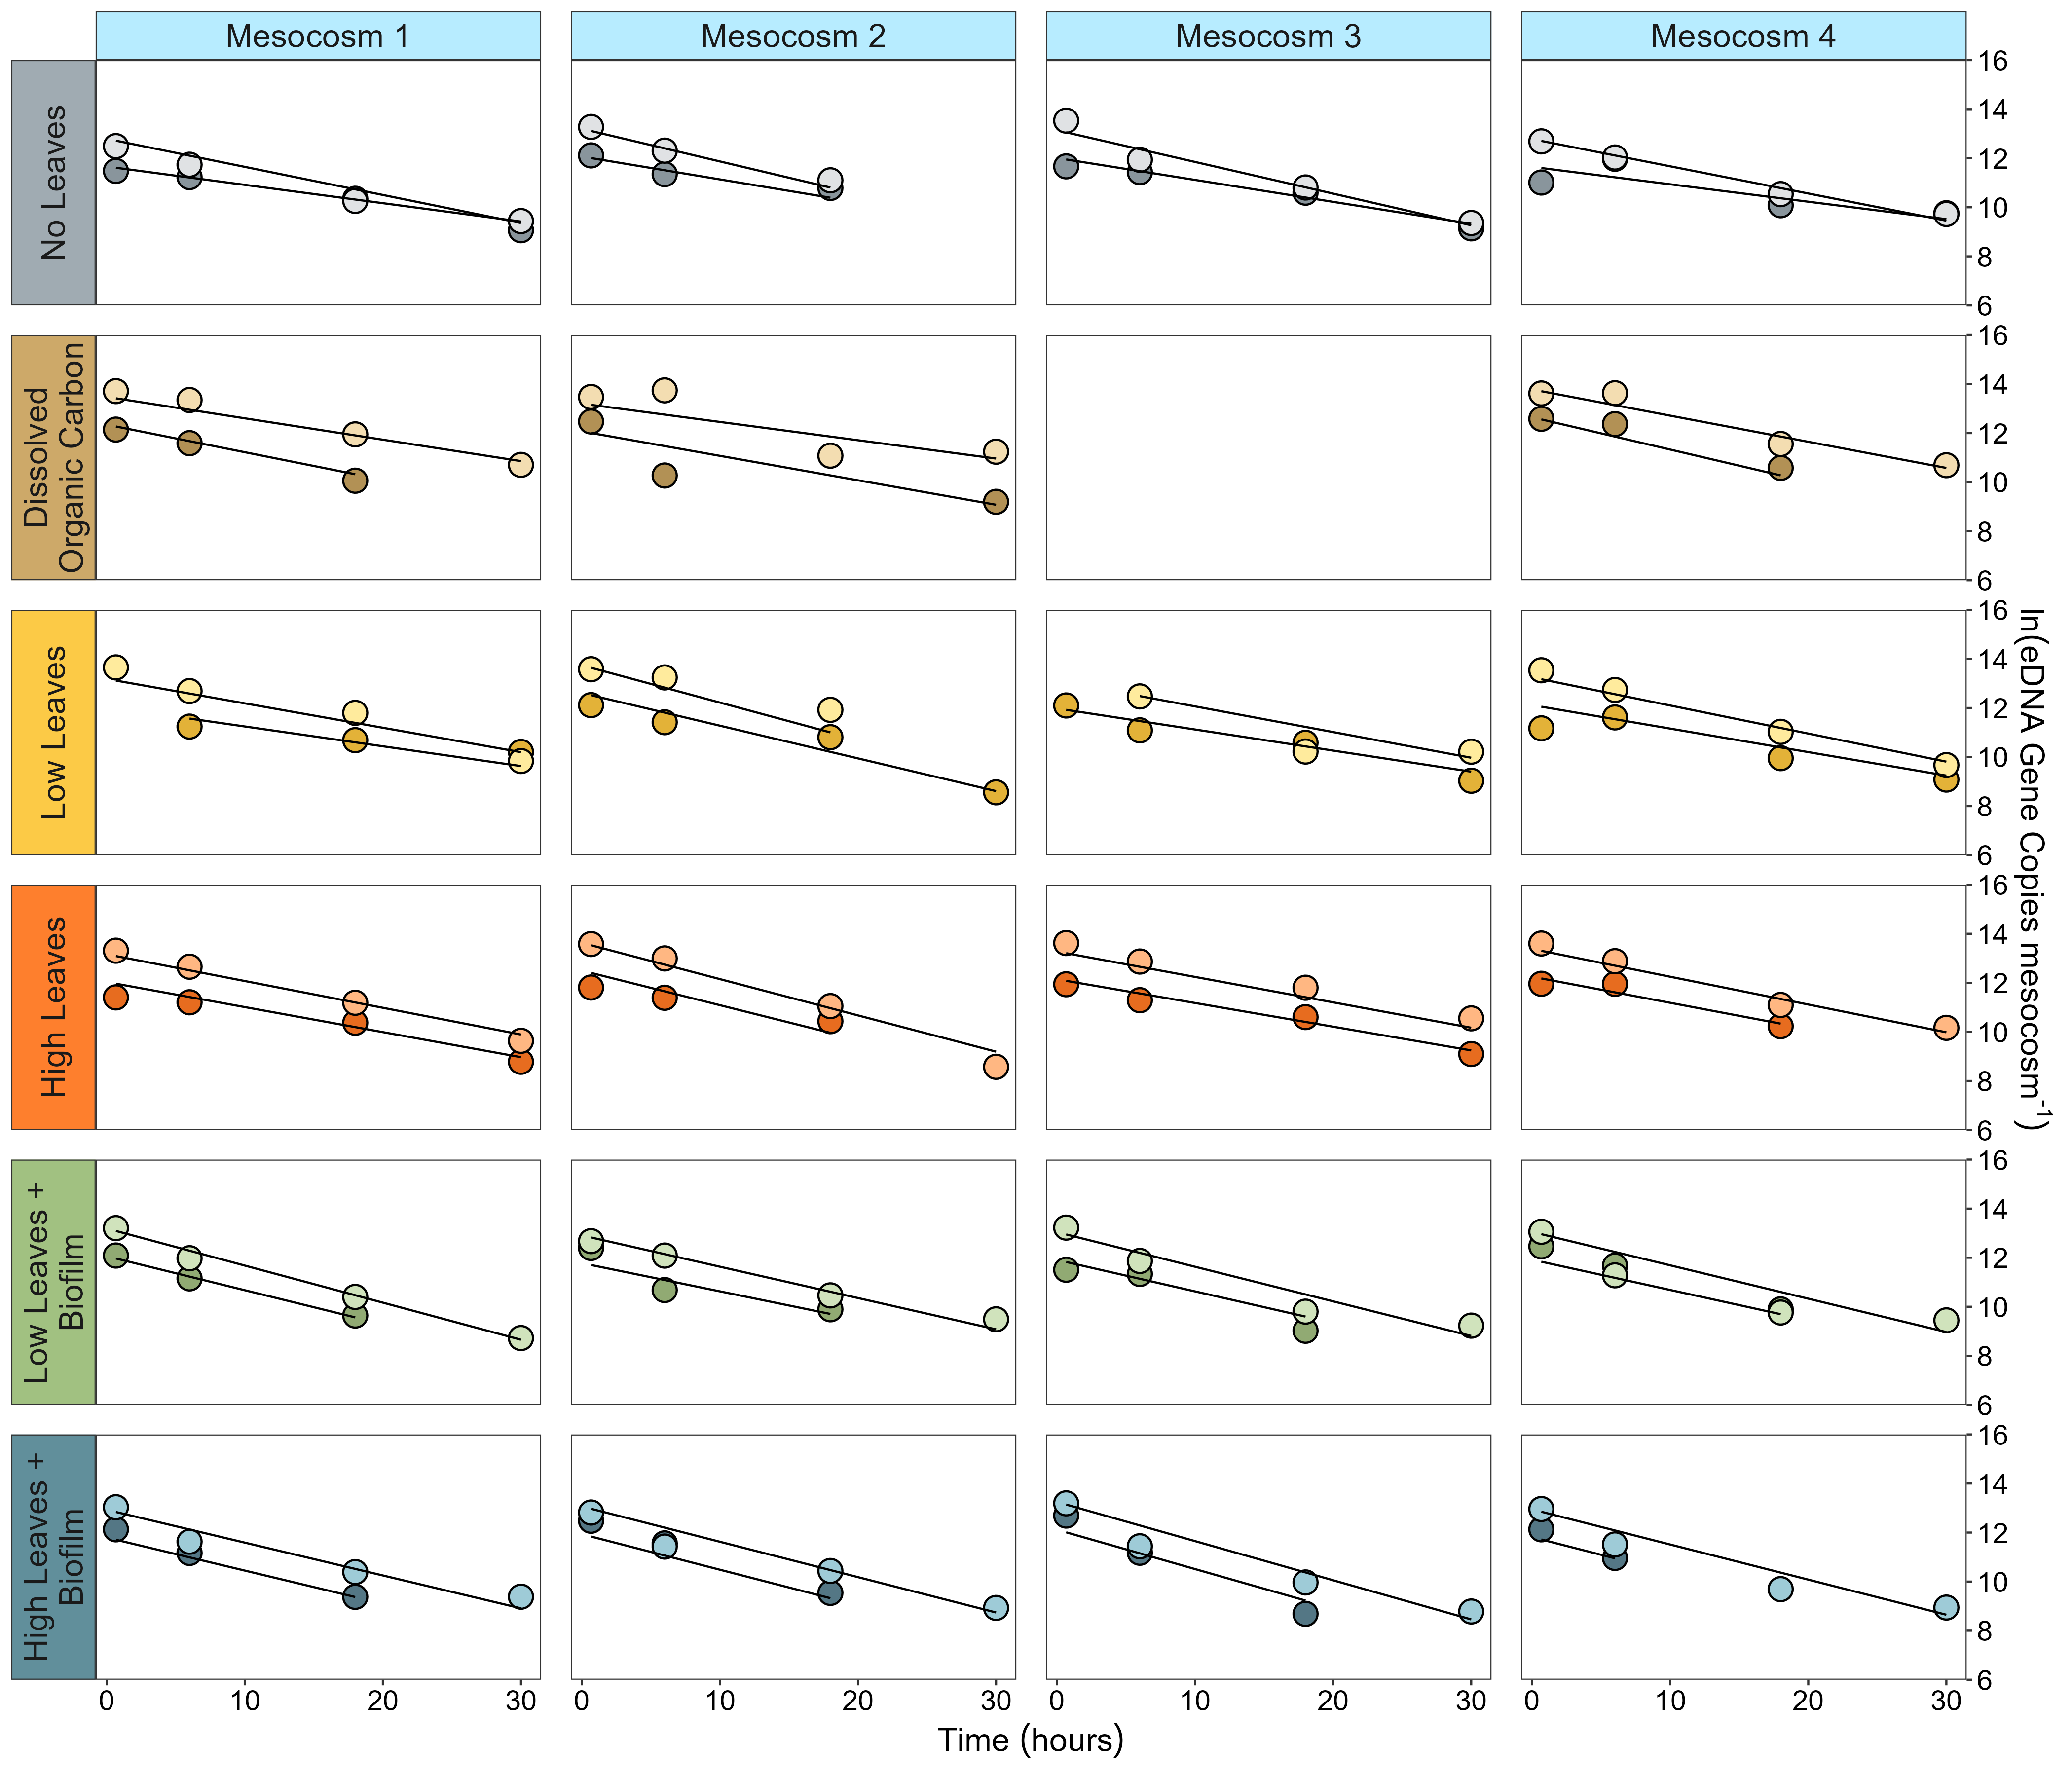
\includegraphics[width=58.33in]{Plots/FigS3}

\begin{Shaded}
\begin{Highlighting}[]
\NormalTok{Fit.plot.Sthd }\OtherTok{\textless{}{-}} \FunctionTok{ggplot}\NormalTok{(fit }\SpecialCharTok{\%\textgreater{}\%} \FunctionTok{subset}\NormalTok{(Target }\SpecialCharTok{==} \StringTok{"STHD"}\NormalTok{), }\FunctionTok{aes}\NormalTok{(}\AttributeTok{x=}\NormalTok{Time.hr, }\AttributeTok{y=}\NormalTok{LNGc.meso, }\AttributeTok{fill=}\FunctionTok{interaction}\NormalTok{(Treatment,Size)))}\SpecialCharTok{+}
  \FunctionTok{geom\_point}\NormalTok{(}\AttributeTok{size=}\DecValTok{5}\NormalTok{, }\AttributeTok{shape=}\DecValTok{21}\NormalTok{, }\AttributeTok{stroke=}\FloatTok{0.75}\NormalTok{)}\SpecialCharTok{+}
  \FunctionTok{geom\_line}\NormalTok{(}\FunctionTok{aes}\NormalTok{(}\AttributeTok{x =}\NormalTok{ Time.hr, }\AttributeTok{y =}\NormalTok{ Conditional\_Prediction, }\AttributeTok{color=}\NormalTok{Size, }\AttributeTok{linetype=}\StringTok{"dashed"}\NormalTok{))}\SpecialCharTok{+}
  \FunctionTok{theme\_bw}\NormalTok{()}\SpecialCharTok{+}\FunctionTok{theme}\NormalTok{(}\AttributeTok{panel.grid.major =} \FunctionTok{element\_blank}\NormalTok{(), }\AttributeTok{panel.grid.minor =} \FunctionTok{element\_blank}\NormalTok{())}\SpecialCharTok{+}
  \FunctionTok{scale\_fill\_manual}\NormalTok{(}\AttributeTok{values=}\NormalTok{p9}\FloatTok{.5}\NormalTok{)}\SpecialCharTok{+}
  \FunctionTok{scale\_color\_manual}\NormalTok{(}\AttributeTok{values=}\FunctionTok{c}\NormalTok{(}\StringTok{"black"}\NormalTok{,}\StringTok{"black"}\NormalTok{))}\SpecialCharTok{+}
  \FunctionTok{scale\_linetype\_manual}\NormalTok{(}\AttributeTok{values=}\FunctionTok{c}\NormalTok{(}\StringTok{"solid"}\NormalTok{,}\StringTok{"dashed"}\NormalTok{))}\SpecialCharTok{+}
  \FunctionTok{ylab}\NormalTok{(}\FunctionTok{expression}\NormalTok{(}\FunctionTok{ln}\NormalTok{(eDNA}\SpecialCharTok{\textasciitilde{}}\NormalTok{Gene}\SpecialCharTok{\textasciitilde{}}\NormalTok{Copies}\SpecialCharTok{\textasciitilde{}}\NormalTok{mesocosm}\SpecialCharTok{\^{}}\StringTok{"{-}1"}\NormalTok{)))}\SpecialCharTok{+}
  \FunctionTok{xlab}\NormalTok{(}\FunctionTok{expression}\NormalTok{(Time}\SpecialCharTok{\textasciitilde{}}\NormalTok{(hours)))}\SpecialCharTok{+}
  \FunctionTok{theme}\NormalTok{(}\AttributeTok{axis.text.y=}\FunctionTok{element\_text}\NormalTok{(}\AttributeTok{size=}\DecValTok{14}\NormalTok{,}\AttributeTok{color=}\StringTok{"black"}\NormalTok{))}\SpecialCharTok{+}
  \FunctionTok{theme}\NormalTok{(}\AttributeTok{axis.text.x=}\FunctionTok{element\_text}\NormalTok{(}\AttributeTok{size=}\DecValTok{14}\NormalTok{,}\AttributeTok{color=}\StringTok{"black"}\NormalTok{))}\SpecialCharTok{+}
  \FunctionTok{theme}\NormalTok{(}\AttributeTok{axis.title.x=}\FunctionTok{element\_text}\NormalTok{(}\AttributeTok{size=}\DecValTok{16}\NormalTok{,}\AttributeTok{color=}\StringTok{"black"}\NormalTok{))}\SpecialCharTok{+}
  \FunctionTok{theme}\NormalTok{(}\AttributeTok{axis.title.y=}\FunctionTok{element\_text}\NormalTok{(}\AttributeTok{size=}\DecValTok{16}\NormalTok{,}\AttributeTok{color=}\StringTok{"black"}\NormalTok{))}\SpecialCharTok{+}
  \FunctionTok{theme}\NormalTok{(}\AttributeTok{legend.position=}\StringTok{"none"}\NormalTok{)}\SpecialCharTok{+}
  \FunctionTok{scale\_y\_continuous}\NormalTok{(}\AttributeTok{expand=}\FunctionTok{c}\NormalTok{(}\DecValTok{0}\NormalTok{,}\DecValTok{0}\NormalTok{),}\AttributeTok{limits=}\FunctionTok{c}\NormalTok{(}\DecValTok{6}\NormalTok{,}\DecValTok{16}\NormalTok{), }\AttributeTok{position =} \StringTok{"right"}\NormalTok{)}\SpecialCharTok{+}
  \DocumentationTok{\#\#\#These lines facet the graph}
  \FunctionTok{facet\_grid}\NormalTok{(Treatment}\SpecialCharTok{\textasciitilde{}}\NormalTok{Row, }\AttributeTok{switch=}\StringTok{"y"}\NormalTok{, }\AttributeTok{labeller =} \FunctionTok{as\_labeller}\NormalTok{(headernames))}\SpecialCharTok{+}
  \FunctionTok{theme}\NormalTok{(}\AttributeTok{strip.text.x =} \FunctionTok{element\_text}\NormalTok{(}\AttributeTok{size=}\DecValTok{16}\NormalTok{),}
        \AttributeTok{strip.text.y =} \FunctionTok{element\_text}\NormalTok{(}\AttributeTok{size=}\DecValTok{16}\NormalTok{))}\SpecialCharTok{+}
  \FunctionTok{theme}\NormalTok{(}\AttributeTok{strip.background =}\FunctionTok{element\_rect}\NormalTok{(}\AttributeTok{fill=}\StringTok{"white"}\NormalTok{))}\SpecialCharTok{+}
  \FunctionTok{theme}\NormalTok{(}\AttributeTok{panel.spacing =} \FunctionTok{unit}\NormalTok{(}\DecValTok{1}\NormalTok{, }\StringTok{"lines"}\NormalTok{))}
\CommentTok{\#Add colors to facet grid}
\NormalTok{g }\OtherTok{\textless{}{-}} \FunctionTok{facetColor}\NormalTok{(Fit.plot.Sthd, }\FunctionTok{c}\NormalTok{(}\StringTok{"\#E8CDE9"}\NormalTok{,}\StringTok{"\#E8CDE9"}\NormalTok{,}\StringTok{"\#E8CDE9"}\NormalTok{,}\StringTok{"\#E8CDE9"}\NormalTok{,p7))}
\FunctionTok{ggsave}\NormalTok{(}\AttributeTok{filename=}\FunctionTok{paste0}\NormalTok{(plots.dir,}\StringTok{"/FigS4.png"}\NormalTok{), g, }\AttributeTok{width =} \DecValTok{14}\NormalTok{, }\AttributeTok{height =} \DecValTok{12}\NormalTok{, }\AttributeTok{units =} \FunctionTok{c}\NormalTok{(}\StringTok{"in"}\NormalTok{))}

\NormalTok{knitr}\SpecialCharTok{::}\FunctionTok{include\_graphics}\NormalTok{(}\FunctionTok{paste0}\NormalTok{(plots.dir,}\StringTok{"/FigS4.png"}\NormalTok{))}
\end{Highlighting}
\end{Shaded}

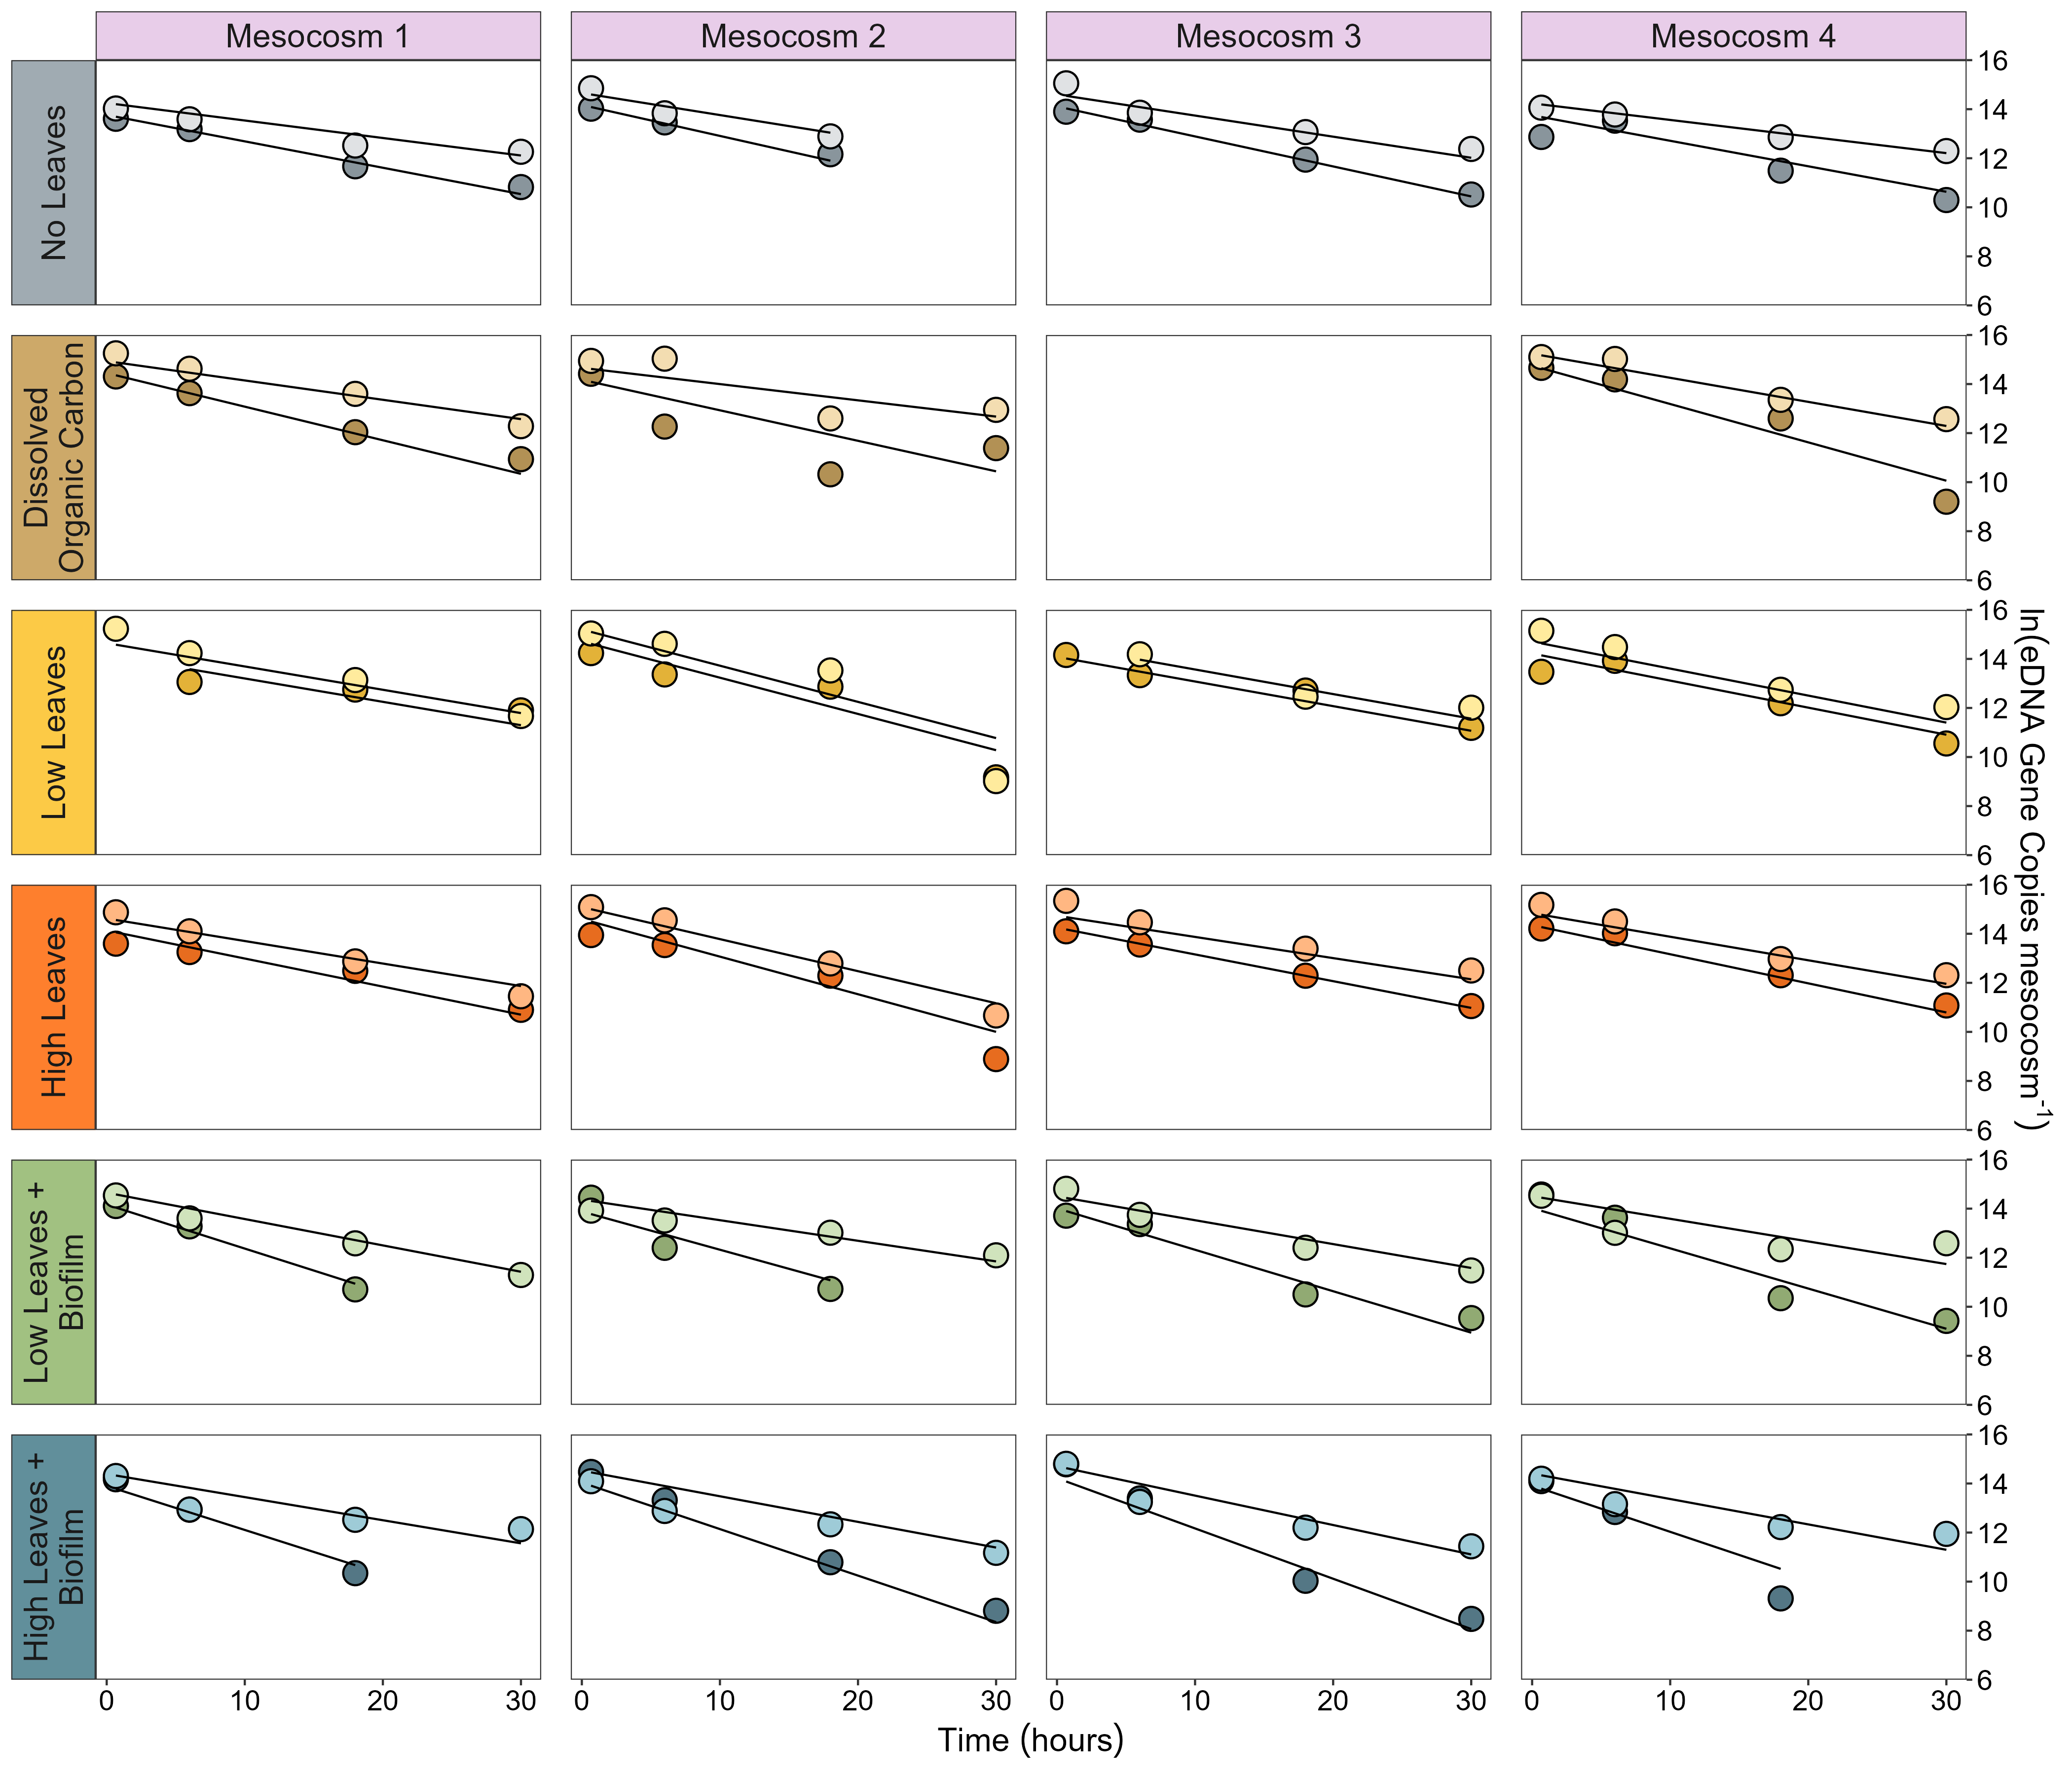
\includegraphics[width=58.33in]{Plots/FigS4}

\end{document}
